%% 
%% Copyright 2007, 2008, 2009 Elsevier Ltd
%% 
%% This file is part of the 'Elsarticle Bundle'.
%% ---------------------------------------------
%% 
%% It may be distributed under the conditions of the LaTeX Project Public
%% License, either version 1.2 of this license or (at your option) any
%% later version.  The latest version of this license is in
%%    http://www.latex-project.org/lppl.txt
%% and version 1.2 or later is part of all distributions of LaTeX
%% version 1999/12/01 or later.
%% 
%% The list of all files belonging to the 'Elsarticle Bundle' is
%% given in the file `manifest.txt'.
%% 

%% Template article for Elsevier's document class `elsarticle'
%% with numbered style bibliographic references
%% SP 2008/03/01

\documentclass[preprint,1p]{elsarticle}
\biboptions{numbers,sort&compress}

%% Use the option review to obtain double line spacing
%% \documentclass[authoryear,preprint,review,12pt]{elsarticle}

%% Use the options 1p,twocolumn; 3p; 3p,twocolumn; 5p; or 5p,twocolumn
%% for a journal layout:
%% \documentclass[final,1p,times]{elsarticle}
%% \documentclass[final,1p,times,twocolumn]{elsarticle}
%% \documentclass[final,3p,times]{elsarticle}
%% \documentclass[final,3p,times,twocolumn]{elsarticle}
%% \documentclass[final,5p,times]{elsarticle}
%% \documentclass[final,5p,times,twocolumn]{elsarticle}

%% For including figures, graphicx.sty has been loaded in
%% elsarticle.cls. If you prefer to use the old commands
%% please give \usepackage{epsfig}

%% The amssymb package provides various useful mathematical symbols
\usepackage{amssymb}
\usepackage{lineno}
\usepackage{hyperref}
\usepackage[percent]{overpic}

%% The amsthm package provides extended theorem environments
%% \usepackage{amsthm}

%% The lineno packages adds line numbers. Start line numbering with
%% \begin{linenumbers}, end it with \end{linenumbers}. Or switch it on
%% for the whole article with \linenumbers.
%% \usepackage{lineno}

\journal{Nucl. Instrum. Meth. A}

\begin{document}
\linenumbers

\begin{frontmatter}

%% Title, authors and addresses

%% use the tnoteref command within \title for footnotes;
%% use the tnotetext command for theassociated footnote;
%% use the fnref command within \author or \address for footnotes;
%% use the fntext command for theassociated footnote;
%% use the corref command within \author for corresponding author footnotes;
%% use the cortext command for theassociated footnote;
%% use the ead command for the email address,
%% and the form \ead[url] for the home page:
%% \title{Title\tnoteref{label1}}
%% \tnotetext[label1]{}
%% \author{Name\corref{cor1}\fnref{label2}}
%% \ead{email address}
%% \ead[url]{home page}
%% \fntext[label2]{}
%% \cortext[cor1]{}
%% \address{Address\fnref{label3}}
%% \fntext[label3]{}

\title{Test Beam Studies Of 50~$\mu m$ LGAD sensors.}

%% use optional labels to link authors explicitly to addresses:
%% \author[label1,label2]{}
%% \address[label1]{}
%% \address[label2]{}

\author[1]{A.~Apresyan\corref{cor}}\ead{apresyan@fnal.gov}
\author[2]{S.~Xie}
\author[2]{C.~Pena}
%\author[5]{R.~Arcidiacono}
\author[5]{N.~Cartiglia}
\author[1]{G.~Derylo}
%\author[5]{M.~Ferrero}
\author[4]{P.~Freeman}
\author[4]{Z.~Galloway}
%\author[4]{Y.~Ghao}
\author[3]{H.~Al Ghoul}
\author[1]{L.~Gray}
%\author[4]{C.~Labitan}
\author[1]{S.~Los}
%\author[4]{Z.~Luce}
%\author[5]{M.~Mandurrino}
%\author[2]{A.~Mangu}
%\author[4]{F.~Martinez-Mckinney}
\author[3]{N.~Minafra}
%\author[1]{A.~Prosser}
%\author[1]{R.~Rivera}
\author[3]{C.~Royon}
\author[4]{H.~Sadrozinski}
\author[4]{A.~Seiden}
%\author[5]{V.~Sola}
\author[2]{M.~Spiropulu}
%\author[4]{E.~Spencer}
%\author[5]{A.~Staiano}
\author[1]{L.~Uplegger}
%\author[4]{M.~Wilder}

\address[1]{Fermi National Accelerator Laboratory, Batavia, IL, USA}
\address[2]{California Institute of Technology, Pasadena, CA, USA}
\address[3]{University of Kansas, KS, USA}
\address[4]{SCIPP, University of California Santa Cruz, CA, USA}
\address[5]{Università di Torino, Torino, Italy}

\cortext[cor]{Corresponding author}

\begin{abstract}
%% Text of abstract
The high luminosity upgrade of the Large Hadron Collider (HL-LHC) at CERN is
expected to provide instantaneous luminosities of $5\times 10^{34}$ cm$^{-2}$
s$^{-1}$. The high luminosities expected at the HL-LHC will be accompanied by a
factor of $5$ to $10$ more pileup compared with LHC conditions in $2015$,
further increasing the challenge for particle identification and event
reconstruction. Precision timing allows to extend calorimetric measurements into
such a high density environment by subtracting the energy deposits from pileup
interactions. Calorimeters employing silicon as the active component have
recently become a viable choice for the HL-LHC and future collider experiments
which face very high radiation environments. In this article, we present studies
of basic calorimetric and precision timing measurements using a prototype
composed of tungsten absorber and silicon sensor as the active medium. We show
that for the bulk of electromagnetic showers induced by electrons in the range
of $20$~GeV to $30$~GeV, we can achieve time resolutions better than $25$~ps per
single pad sensor. 

\end{abstract}

\begin{keyword}
%% keywords here, in the form: keyword \sep keyword

%% PACS codes here, in the form: \PACS code \sep code
Silicon \sep Timing \sep LGAD
%% MSC codes here, in the form: \MSC code \sep code
%% or \MSC[2008] code \sep code (2000 is the default)

\end{keyword}

\end{frontmatter}

%% \linenumbers

%% main text
\section{Introduction} 

\section{Test-beam Setup} 

%We performed the test-beam measurements at the Fermilab Test-beam
%Facility%

Test-beam measurements were performed at the Fermilab Test-beam Facility (FTBF)
which provided a $120$~GeV proton beam from the Fermilab Main Injector
accelerator. The Devices Under Test (DUTs) were mounted on a remotely operated
motorized stage, placed inside the pixel telescope detector~\cite{KWAN2016162}.
The latter provides better than 10~$\mu$m position resolution for charged
particles impinging on the DUT. Additionally, a Photek 240 microchannel plate
photomultiplier tube (MCP-PMT)%detector% ~\cite{Anderson:2015gha,
MCPFastCaloNIMA, Ronzhin2015288,Ronzhin201552} was placed furthest downstream,
and provided a very precise reference timestamp. Its precision %was% has been
previously measured to be less than $10$~psec~\cite{Ronzhin2015288}. A schematic
diagram and photograph of the experimental area are shown in
Fig.~\ref{fig:DragonBoxDiagram} and Fig.~\ref{fig:DragonBox}, respectively. 

The DAQ system for the DUTs and the Photek MCP-PMT is based on a CAEN V1742
digitizer board~\cite{CAENDRS}, which provides digitized waveforms sampled at 5
GS/s, and with one ADC count corresponding to 0.25~mV. The CAEN digitizer was voltage-
and time-calibrated using the procedure described in Ref.~\cite{Kim201467}. The
electronic€ time resolution of the CAEN V1742 digitizer was
measured to be less than 4~ps, and thus, its impact on the timing measurements presented in these studies
can be neglected. The DAQ for the pixel telescope is based on the CAPTAN system
developed at Fermilab~\cite{KWAN2016162}. The track-reconstruction is performed
using the Monicelli software package developed specifically for the testbeam
application. 

The beam is resonantly extracted in a slow spill for each Main Injector cycle
delivering a single 4.2 sec long spill per minute. The primary beam (bunched at
53 MHz) consists of high energy protons (120 GeV) at variable intensities
between 1 and 300 kHz. The trigger to both the CAEN V1742 and to the pixel
telescope was provided by a scintillator mounted on a photomultiplier tube,
placed upstream of the DUTs in the beam-line. Due to the limited buffer depth of
the CAEN V1742 board, special care had to be taken in the design of the DAQ
system to ensure that both the DUT and telescope DAQs collect exactly the same
amount of triggers. This was achieved by limiting the trigger rate by
introducting an adjustable dead-time using a custom-designed trigger board. This
trigger board is the combination of a custom FPGA board (the CAPTAN+x, equipped
with multiple FPGA Mezzanine Card connectors and gigabit ethernet connectivity)
mated to a front end board (the NIM+, with multiple inputs and outputs, each
supporting a variety of interface levels such as NIM, LVDS, and TTL). The
combined board is shown in Fig.~\ref{fig:NIM+Captan} and was used to interface to
photomultiplier signals through on-board programmable discriminators, and to form
trigger signals with software configurable time-based veto and pre-scaler event
filtering. We found that at a rate of about 1,500 triggers per spill the CAEN
V1742 and pixel telescope were maintained fully synchronized. Processed data
from the pixel telescope and the DUTs were merged offline by matching the
trigger counters recorded by the two systems.

\begin{figure}[htbp] 
\centering
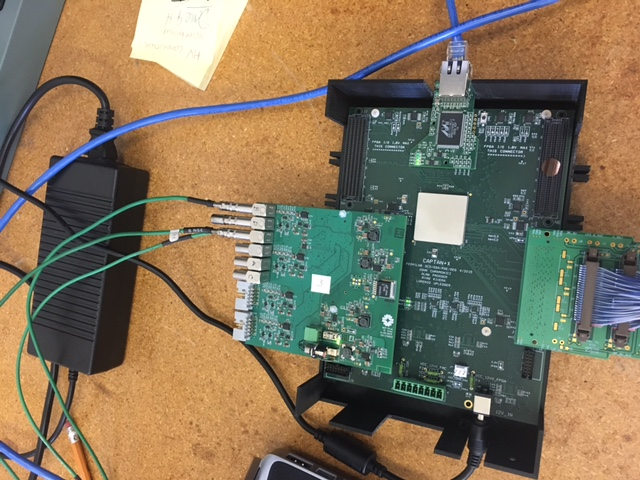
\includegraphics[width=0.5\textwidth, angle=270]{figs/CAPTAN_NIM_Plus.JPG} 
\caption{The custom-made trigger board composed of NIM+ and CAPTAN+x boards.} 
\label{fig:NIM+Captan} 
\end{figure} 




\begin{figure}[htbp] 
\centering
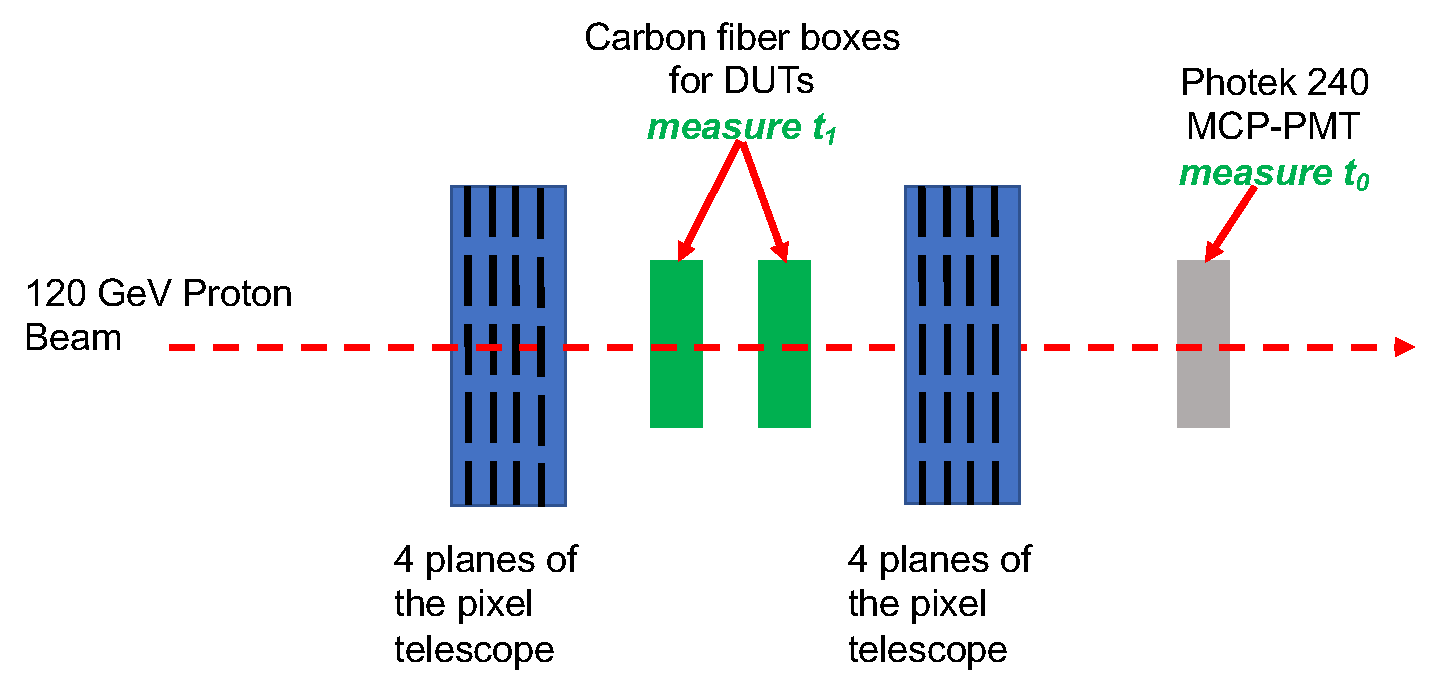
\includegraphics[width=0.75\textwidth]{figs/BeamSetup.pdf} 
\caption{A schematic diagram of the test-beam setup is shown. The $t_0$ and $t_1$ are defined in Section 4.} 
\label{fig:DragonBoxDiagram} 
\end{figure} 

The devices under test (DUT) were placed inside the telescope box described in
Ref.\cite{KWAN2016162}, and mounted on aluminum mechanical support structure.
The telescope box can be moved remotely in both horizontal and vertical
directions, in order to align the DUTs with the beam. The aluminum support
structures for DUT provide both a mechanical stability for the DUTs, and are
equipped with Peltier cooling elements that were used in this study to operate
the DUTs at $-10^{\circ}$ and $-20^{\circ}$~C.

\begin{figure}[htbp] 
\centering
\includegraphics[width=0.75\textwidth]{figs/TB_dragonBox.pdf} 
\caption{A picture of the experimental area. Thea pixel telescope detectors are placed inside the ESD shielded boxes on the two sides of the DUT area. Cooling liquid for the Peltier elements inside the DUT area is provided by the two pipes shown in the picture.} 
\label{fig:DragonBox} 
\end{figure} 


\section{Properties of the tested LGAD sensors}

Sensors manufactured by Hamamatsu (HPK) and CNM were tested during the test beam
experiments. All sensors have active thickness of about 50 $\mu$m. 

{\bf FIXME NICOLO OR HARTMUT: FILL IN DETAILS OF CNM AND HPK SENSORS, PRODUCTION
PROCESS ETC} Details on CNM sensors can be found in Ref.~\cite{CNMSensors,
Cartiglia201783}. Hamamatsu sensors have the following properties... 

Sensors in both single- and four-channel configurations were tested during the
measurements. The CNM single-channel sensors had an active area of 1 mm$^2$ {\bf
FIXME: IS THIS CORRECT SIZE OF CNM SINGLE CHANNEL SENSORS?}, and the HPK
single-channel sensors had a diameter of 1~mm. The dimensions of the four
channel sensors from HPK are shown in Fig.~\ref{fig:Sensors}

\begin{figure}[htbp] 
\centering

\includegraphics[width=0.35\textwidth]{figs/HPK-50DPix.pdf} 
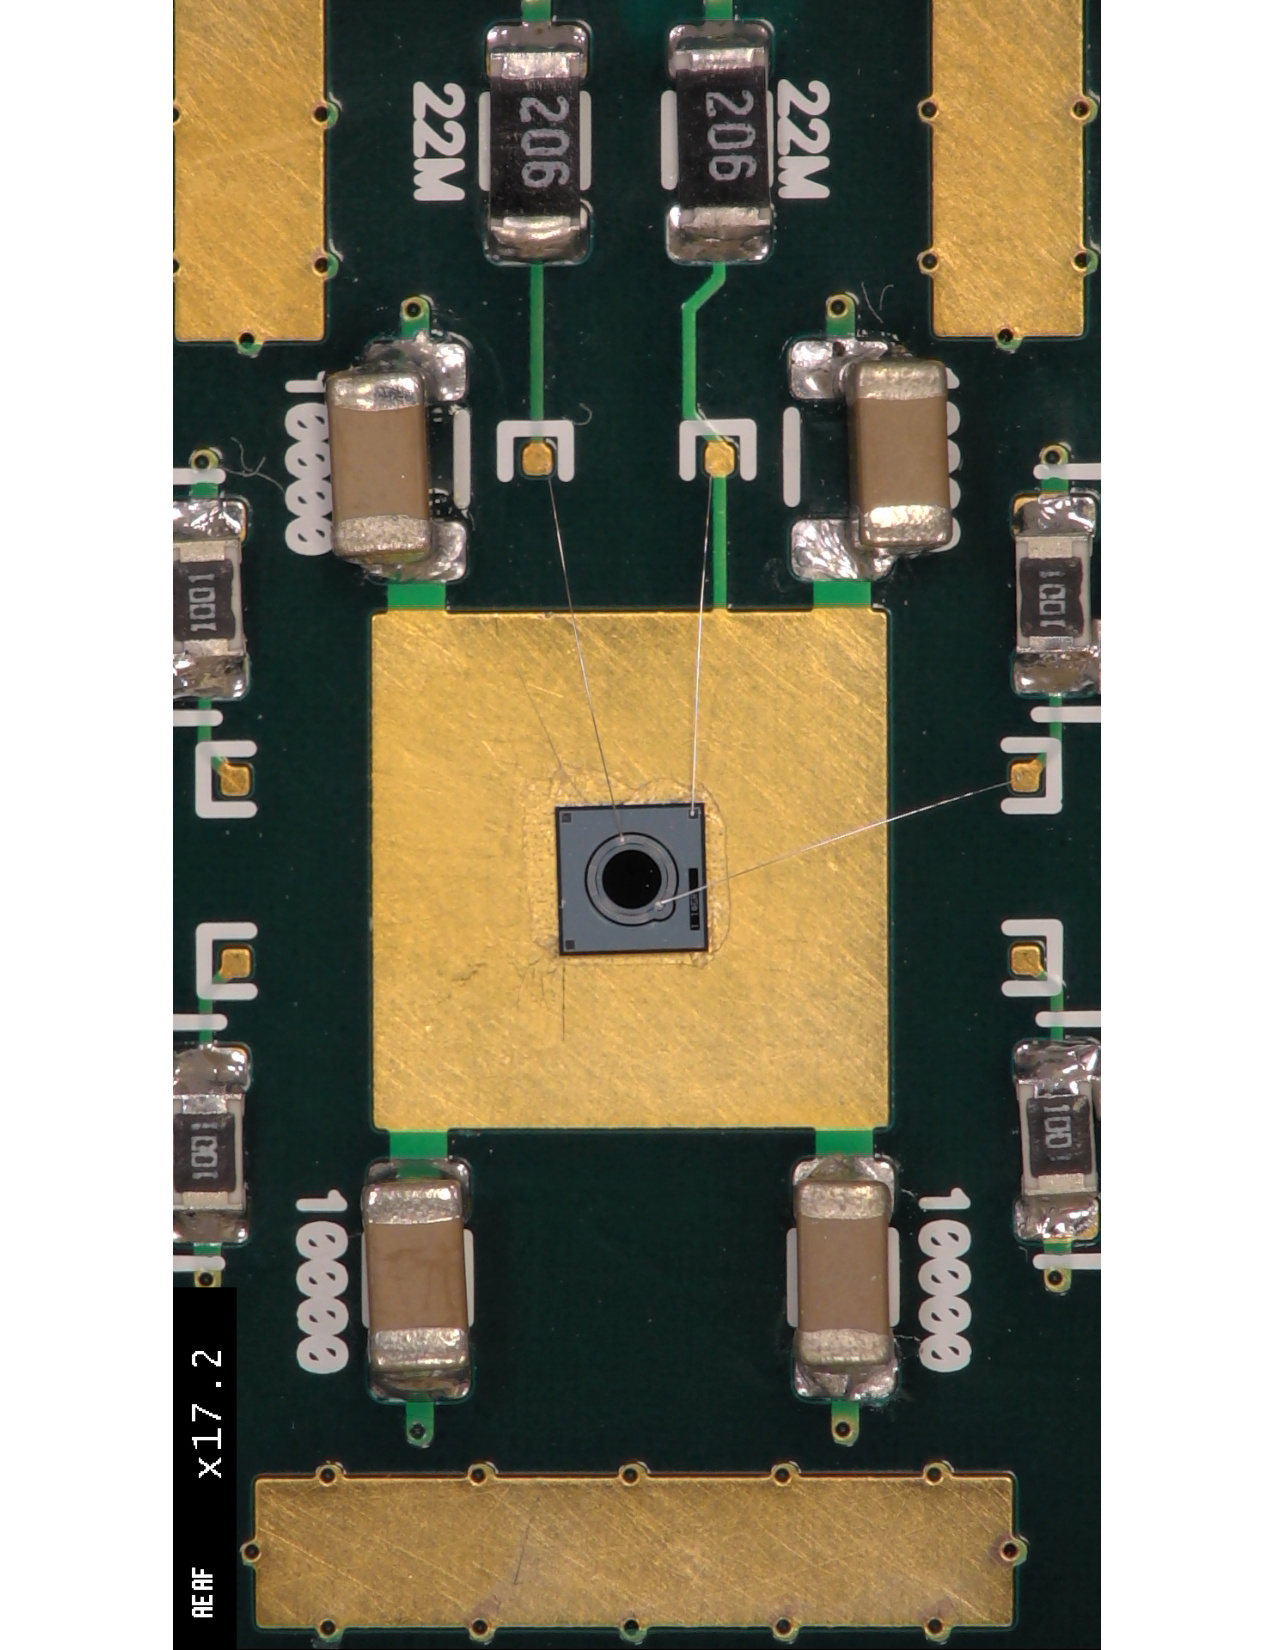
\includegraphics[width=0.48\textwidth]{figs/HPK-50D.pdf} 
\caption{A picture of HPK 50DPix 2x2 array sensor (top), and 50D-GR single sensor (bottom). The pixel labels overlayed on top of the left image are used in the text to identify pixels on the array. Signals from the pixels are read out by the micro-bonds that are connected to the signal pads on the sensors. Signal pads can be seen on the left photograph as four small circles in the center of each pixel. } 
\label{fig:HPK_Sensors} 
\end{figure} 


\section{Read-out boards}

Four boards were used in various measurements presented in this paper, which
were developed at the University of California Santa Cruz (UCSC), University of
Kansas (KU), and at FNAL:

\begin{itemize}
  \item A single-channel USCS board that
was also used in results presented in Ref.~\cite{Cartiglia201783}
\item A four-channel USCS readout board
\item A two-channel KU readout board
\item A 4-channel FNAL readout board.
\end{itemize}

and their detailed description is presented below.  

\textbf {FIXME SERGEY} a paragraph describing the FNAL board. 

\textbf {FIXME NICOLA} a paragraph describing the 2-ch KU board. 

The USCS board 1-channel board is desdcibed in details in
Ref.~\cite{Cartiglia201783}. This board uses discrete components and contains
several features which allow maintaining a wide bandwidth ($\sim$ 2 GHz) and a
low noise even in noisy environments. The inverting amplifier uses a high-speed
SiGe transistor whcih has a trans-impedance of about 470~$\Omega$. 

\textbf {FIXME HARTMUT} a paragraph describing the 4-ch UCSC board. 


\section{Beam test results}

\subsection{Analysis procedure}

The CAEN digitizer is voltage and time calibrated using the procedure described
in Ref.~\cite{Kim201467}. The time for the reference Photek MCP-PMT detector is
obtained by fitting the peak region of the pulse to a Gaussian function and the
mean parameter of the Gaussian is assigned as the timestamp $t_0$. The time for
signals from the LGAD sensors is obtained by performing a linear fit to the
rising edge of the pulse and the time at which the pulse reaches 30\% of the
maximum amplitude is assigned as its timestamp $t1$ \textbf{FIXME DESCRIBE THE
ALGORITHMS FOR LGADS}. We measured the electronic time resolution of the CAEN
V1742 digitizer as $\sim$4~ps and neglected its impact on the timing
measurements described below. 

Events are required to have a signal in the Photek MCP-PMT consistent with a MIP
signal, and a signal above the noise in LGAD sensors. The MIP signal selection
in Photek MCP-PMT is the same for all runs, since it was always read out
directly by the CAEN digitizer. The signal selection for LGAD boards was
optimized for each board individually, by selecting the MIP signal peak fitted
with a Landau function. 

\subsection{Study of the uniformity of the LGAD sensors}

The characteristic uniformity of the HPK 50D-PIX sensors was studied
using the FNAL readout board. Here, and in the remainder of this article,
whenever a scan of a certain characteristic of the array sensors is presented,
we show the X-axis scan for pixels 1 and 2, and the Y-axis scan for pixels 1 and
3, as defined on the left picture in Fig.~\ref{fig:HPK_Sensors}. The X-axis scan
across pixels 3 and 4, and Y-axis scans across pixels 2 and 4 shown
qualitatevely the same features, and are not shown here. 

The measurements of the particle detection efficiency are shown in
Fig.~\ref{fig:FNAL_HPK50_effXY}. Efficiency is defined as the ratio of events
that register a signal above the noise level in the LGAD sensor to those that
contain a track identified by the pixel telescope pointing at the LGAD sensor.
We observe a flat 100\% efficiency across the whole sensor area. The left edge
of the pixel 1 in Fig.~\ref{fig:FNAL_HPK50_effXY} is outside the acceptance of
the pixel telescop, hence the efficiency curve does not fully cover its surface.
A clear drop in efficiency is observed in the transition region between the two
pixels. The area between two pixels is shown in more detail in
Fig.~\ref{fig:FNAL_HPK50_ZoomeffXY}, and as can be seen, particle detection
efficiency is significantly lower in the transition region between the pixels.

\begin{figure}[htbp] 
\centering
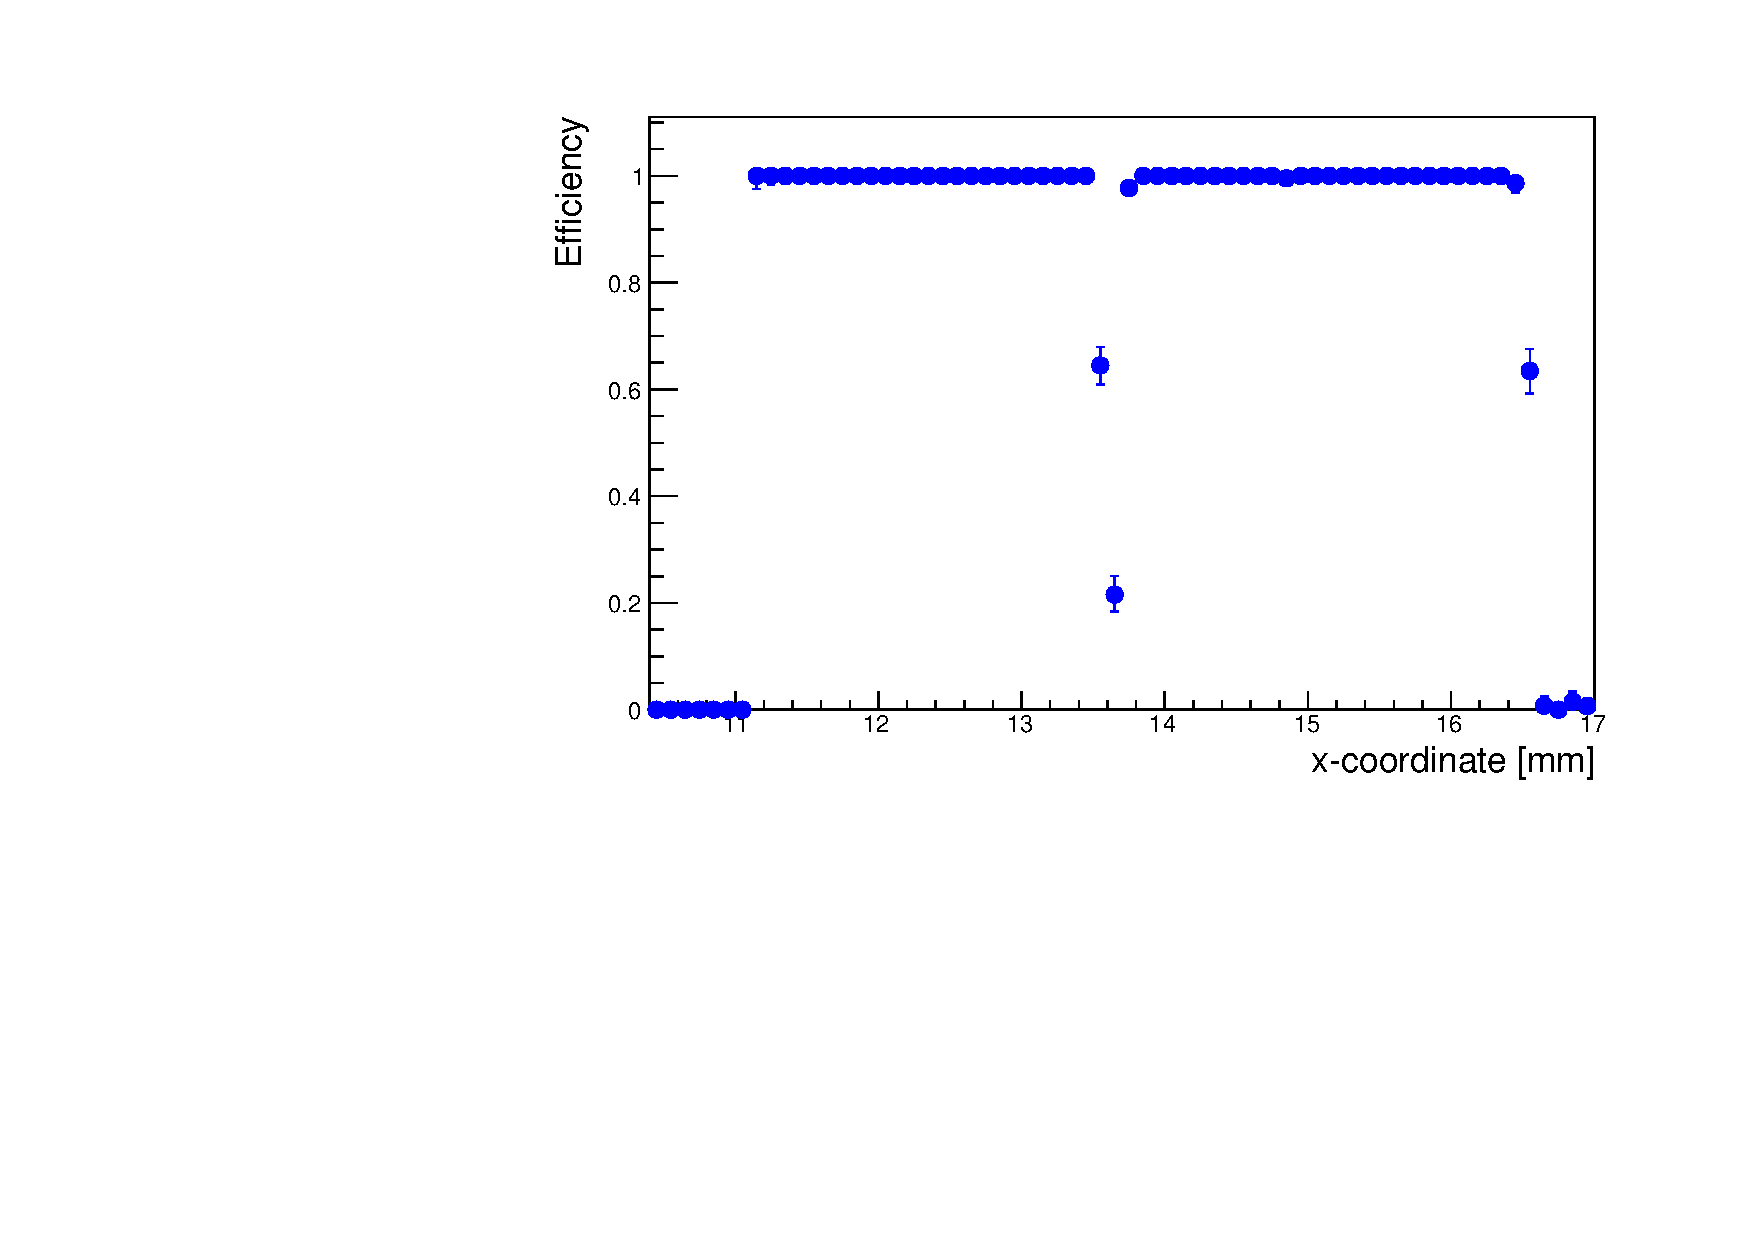
\includegraphics[width=0.48\textwidth]{figs/FNALBoard_HPK50DPix_Run847-891/Eff_vs_X_Ch4_5.pdf} 
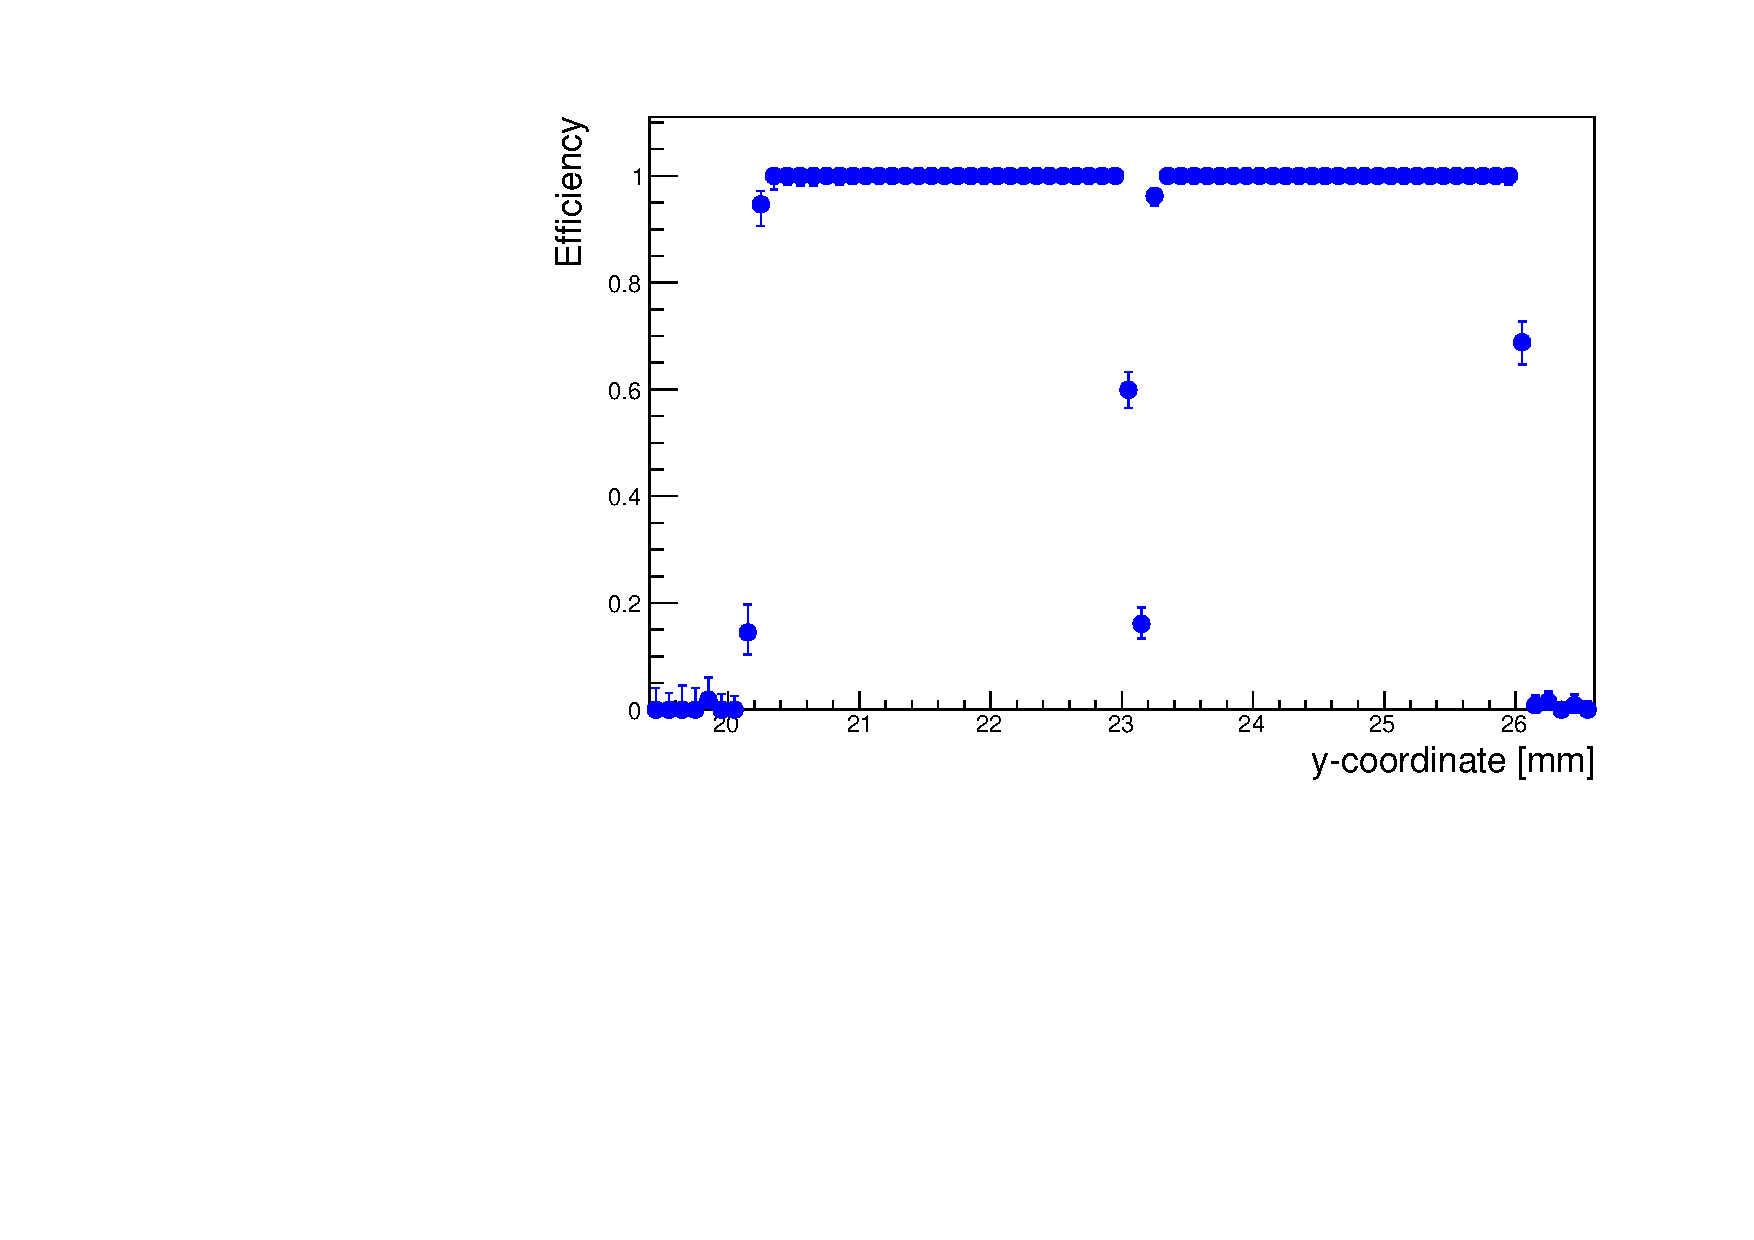
\includegraphics[width=0.48\textwidth]{figs/FNALBoard_HPK50DPix_Run847-891/Eff_vs_Y_Ch3_4.pdf} 
\caption{Efficiency measurement across the X- and Y-axes of the HPK 50D-PIX sensor mounted on the FNAL board. The scan of pixels 1 and 2 along the X-axis, and pixels 1 and 3 along the Y-axis is shown, and pixel numbering scheme is defined in Fig.~\ref{fig:HPK_Sensors}.} 
\label{fig:FNAL_HPK50_effXY} 
\end{figure} 

\begin{figure}[htbp] 
\centering
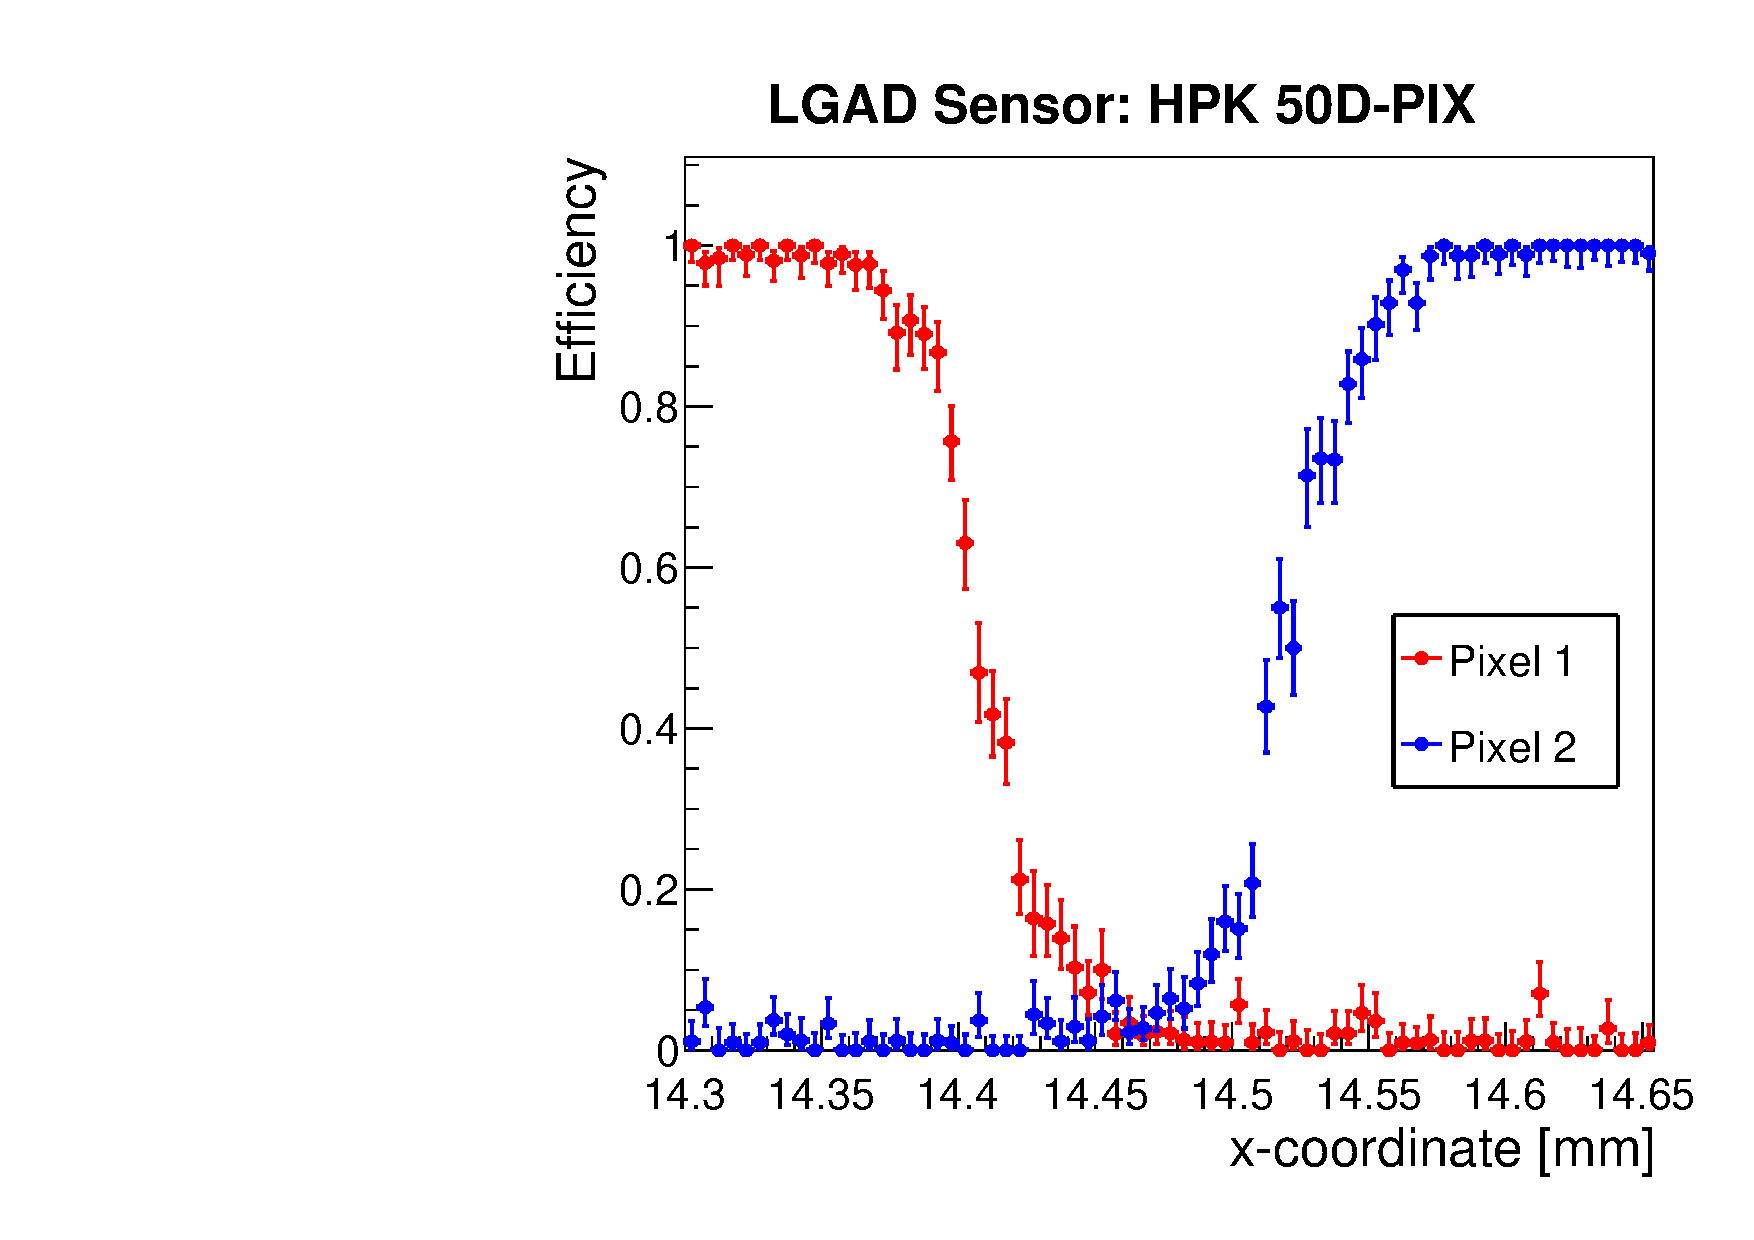
\includegraphics[width=0.48\textwidth]{figs/KUBoard_HPK50DPix_Run638-781/EfficiencyInGap_HPK50DPix.pdf} 
\caption{A zoomed version of the efficiency measurement across the X-axis of the HPK 50D-PIX sensor with 10~$\mu$m binning to show the inter-pixel gap area. Pixel numbering scheme is defined in Fig.~\ref{fig:HPK_Sensors}.} 
\label{fig:FNAL_HPK50_ZoomeffXY} 
\end{figure} 

An important characteristic of the sensors is the unofmity of the signal size
across the sensor surface, which directly impacts the timing characteristics of
the sensor. The distribution of the LGAD signal amplitudes is fit with a Landau
distribution. The post-fit Most Probable Value (MPV) is
plotted in Fig.~\ref{fig:FNAL_HPK50_MPVXY}. A flat response with a uniform
signal size is observed over the whole sensor area.

\begin{figure}[htbp] 
\centering
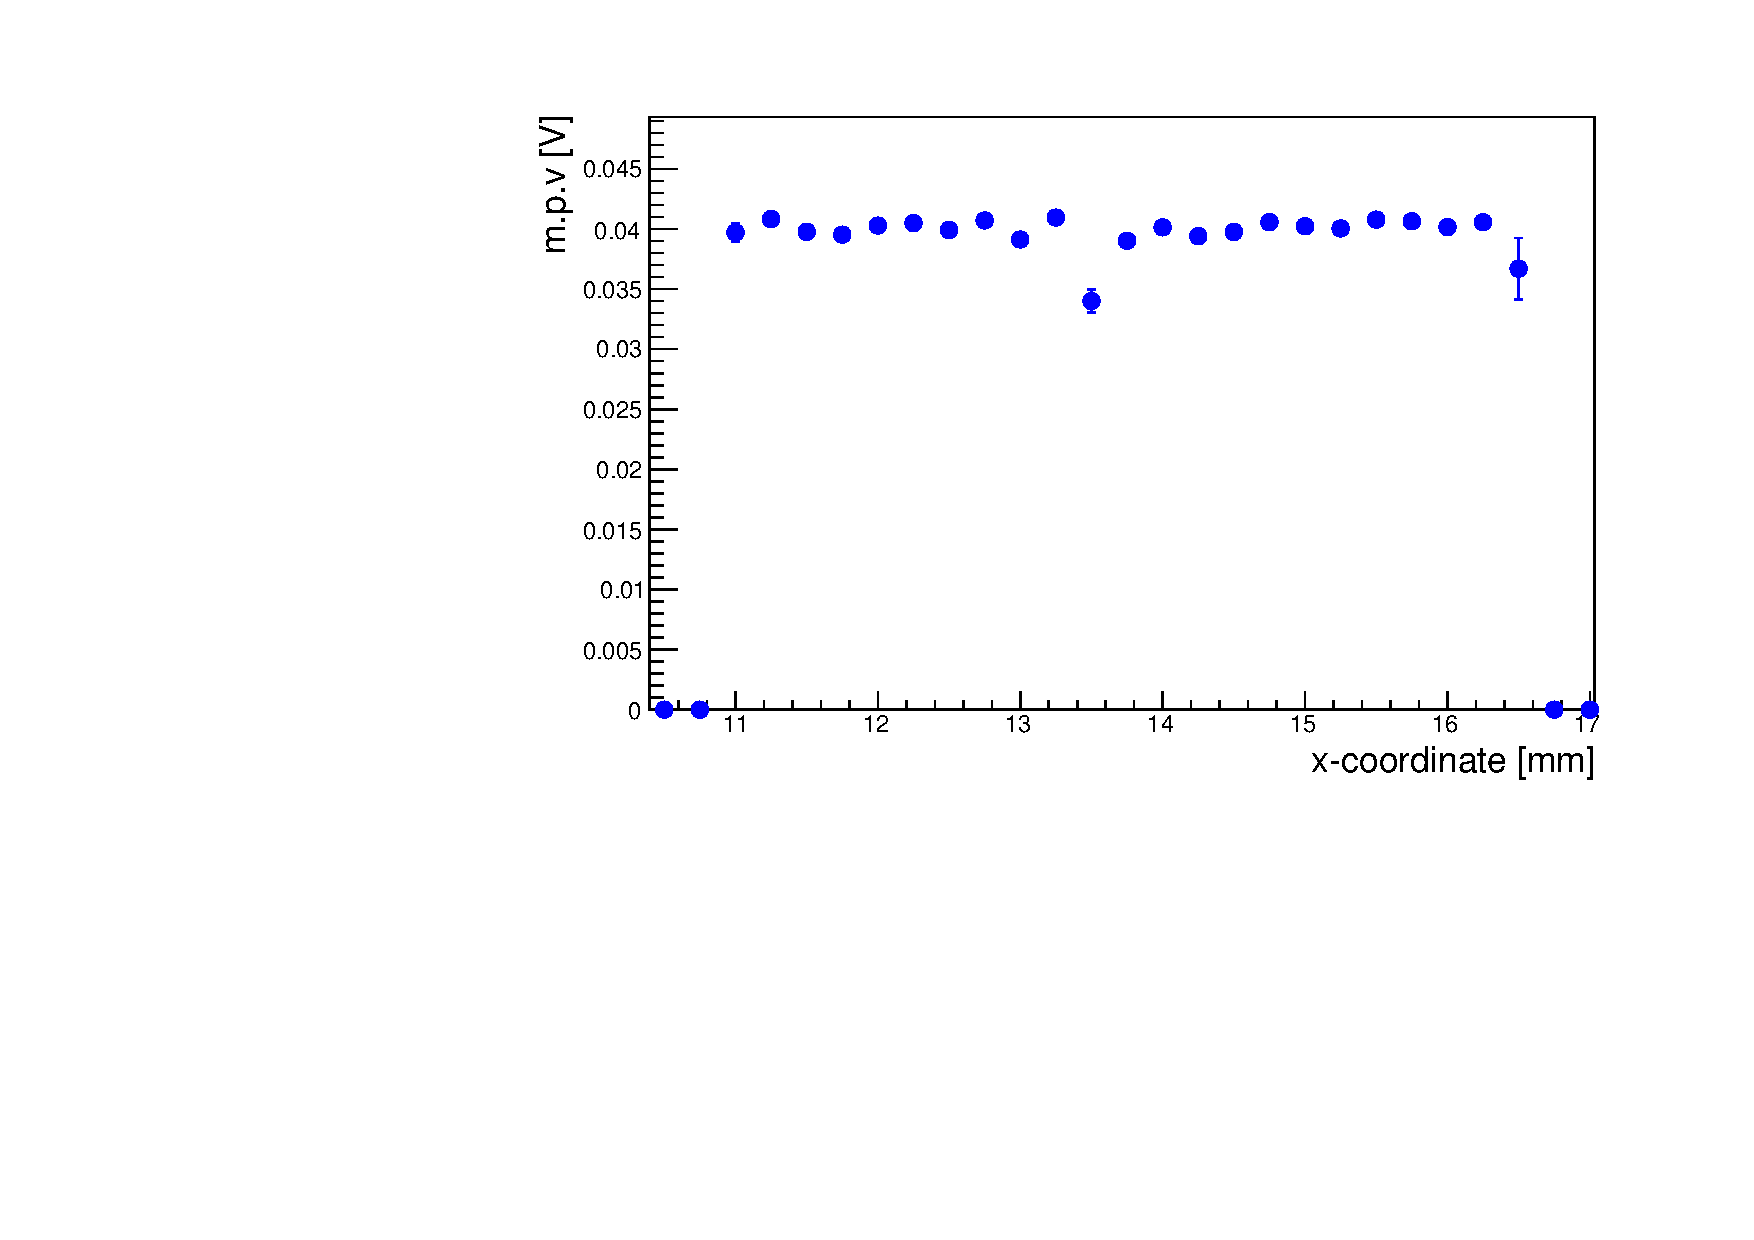
\includegraphics[width=0.48\textwidth]{figs/FNALBoard_HPK50DPix_Run847-891/MPV_vs_X_Ch4_5.pdf} 
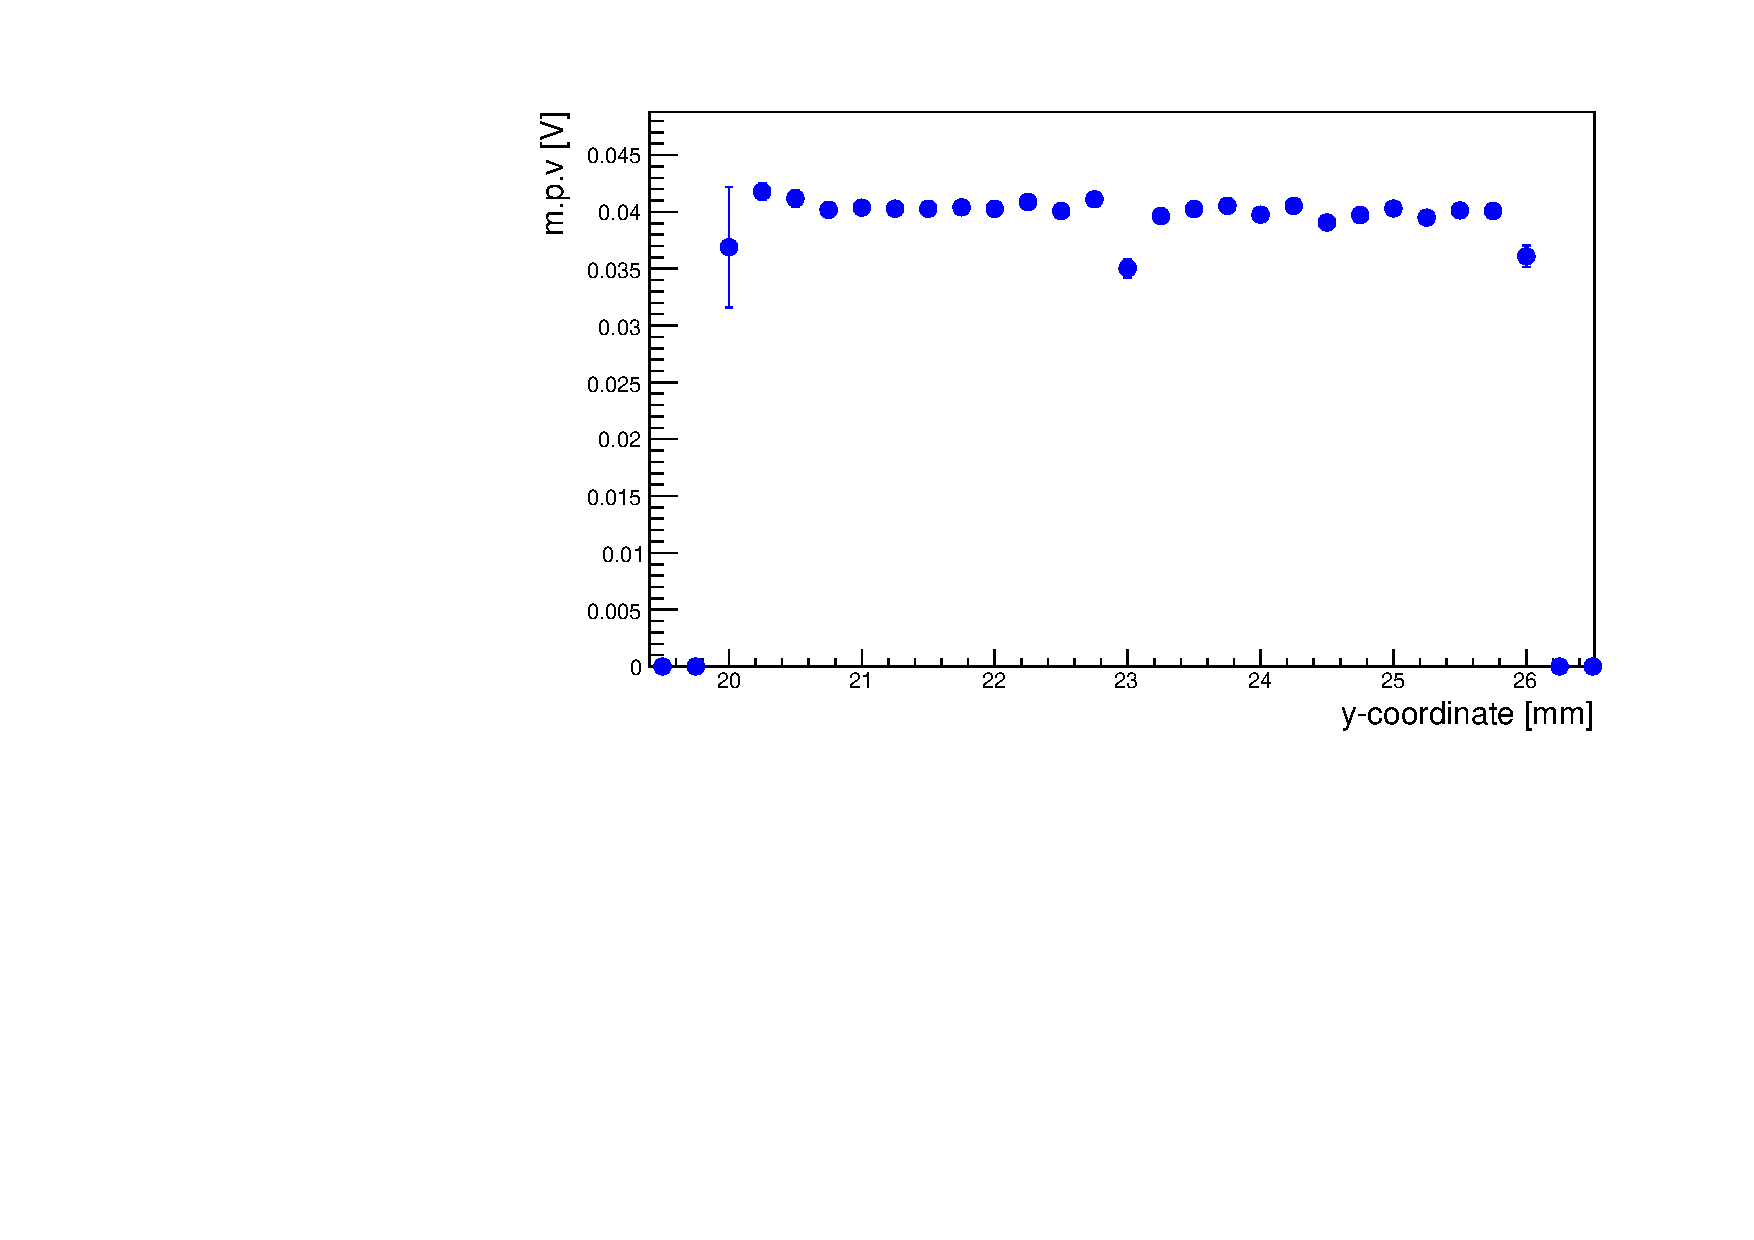
\includegraphics[width=0.48\textwidth]{figs/FNALBoard_HPK50DPix_Run847-891/MPV_vs_Y_Ch3_4.pdf} 
\caption{Signal amplitude MPV measurement across the X- and Y-axes of the HPK 50D-PIX sensor mounted on the FNAL board. The scan of pixels 1 and 2 along the X-axis, and pixels 1 and 3 along the Y-axis is shown, and pixel numberng scheme is defined in Fig.~\ref{fig:HPK_Sensors}.} 
\label{fig:FNAL_HPK50_MPVXY} 
\end{figure} 



The measurement of the time difference between the Photek 240 MCP-PMT time stamp,
and that of the LGAD sensors is shown in Fig.~\ref{fig:FNAL_HPK50_DTXY}. The
micro-bonding scheme of the HPK PIX $2\times 2$ sensors arrays is shown in
Fig.~\ref{fig:HPK_Sensors}. The $\Delta t = t_{1}-t_{0}$ distribution has a distinct shape
where the area under the metalization on top of the sensor -- the gray
area in the center of it -- shows a shift of
about $20$--$30$~psec with respect to non-metalized area. 

\begin{figure}[htbp] 
\centering
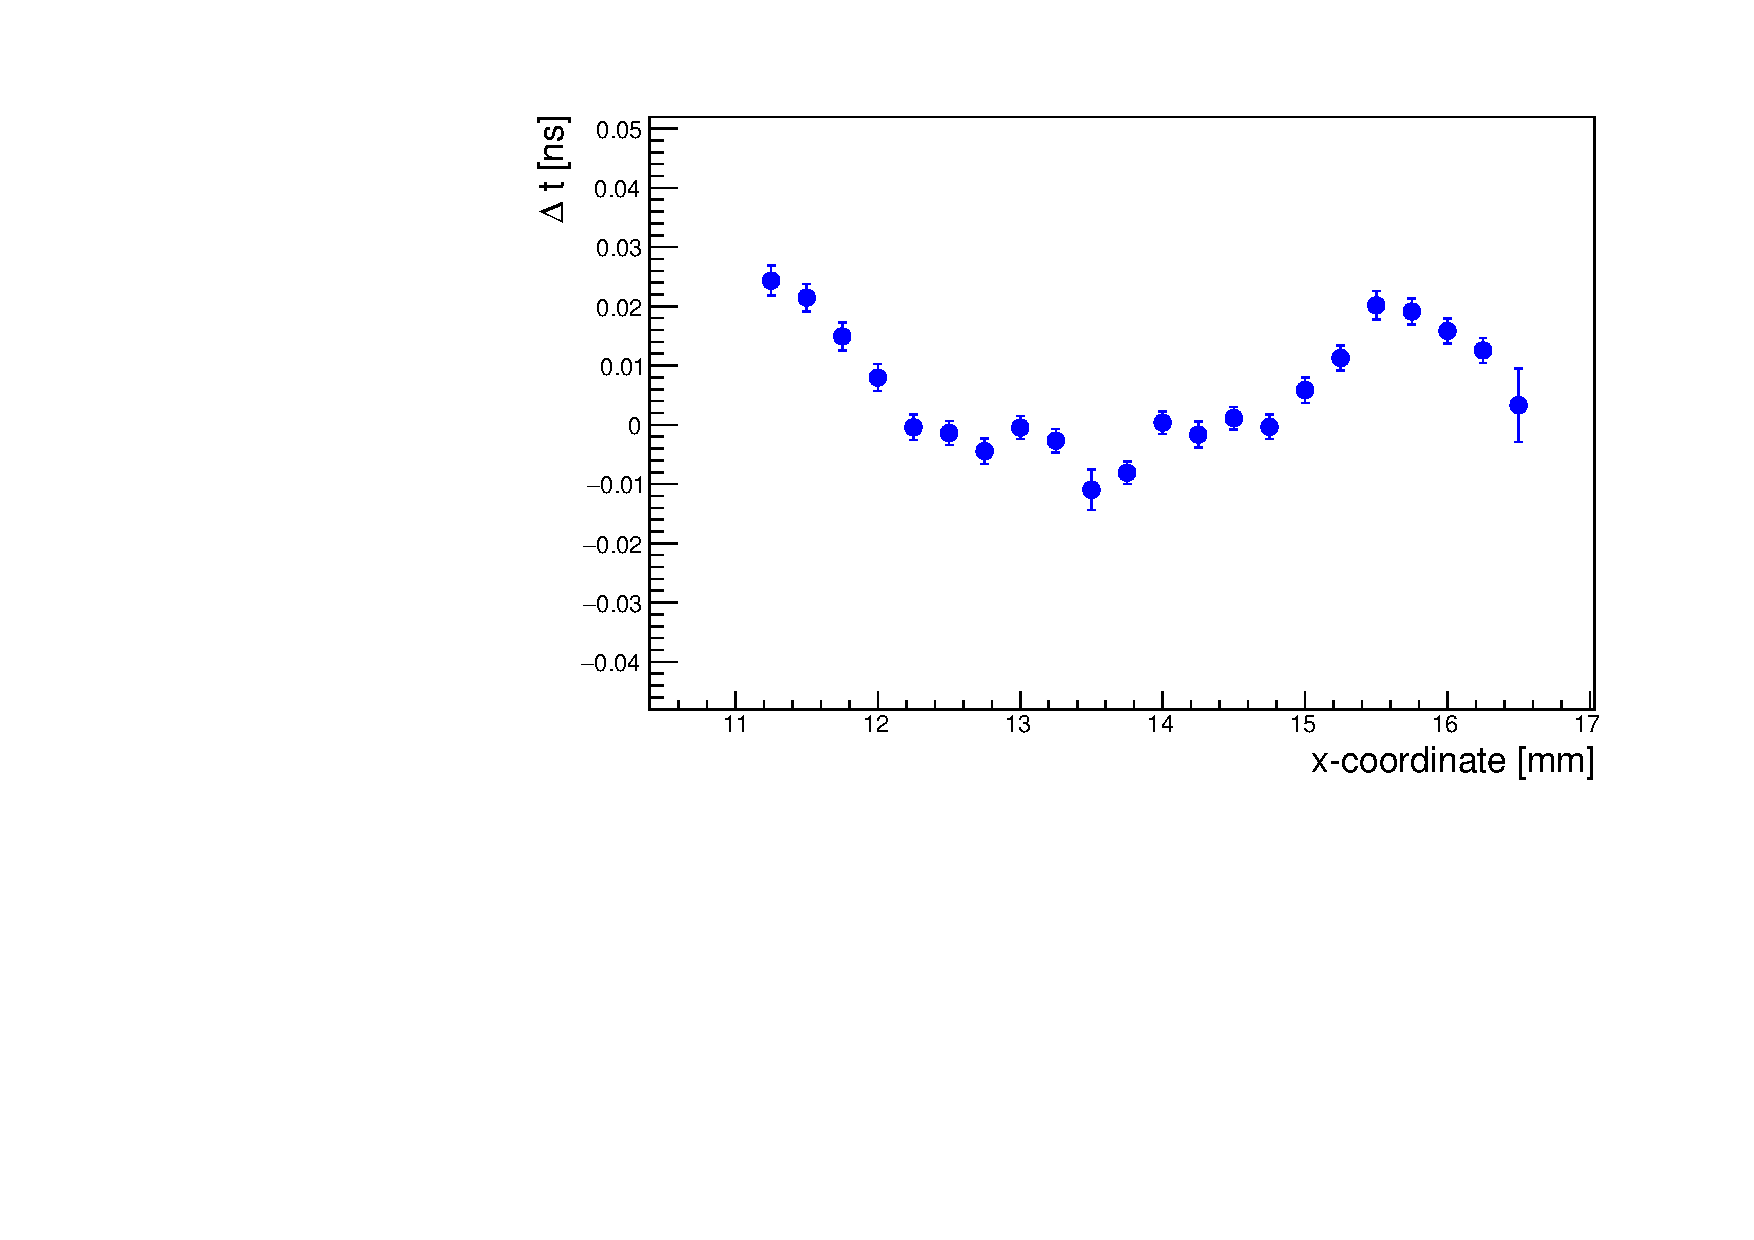
\includegraphics[width=0.48\textwidth]{figs/FNALBoard_HPK50DPix_Run847-891/MeanTime_vs_X_Ch4_5.pdf} 
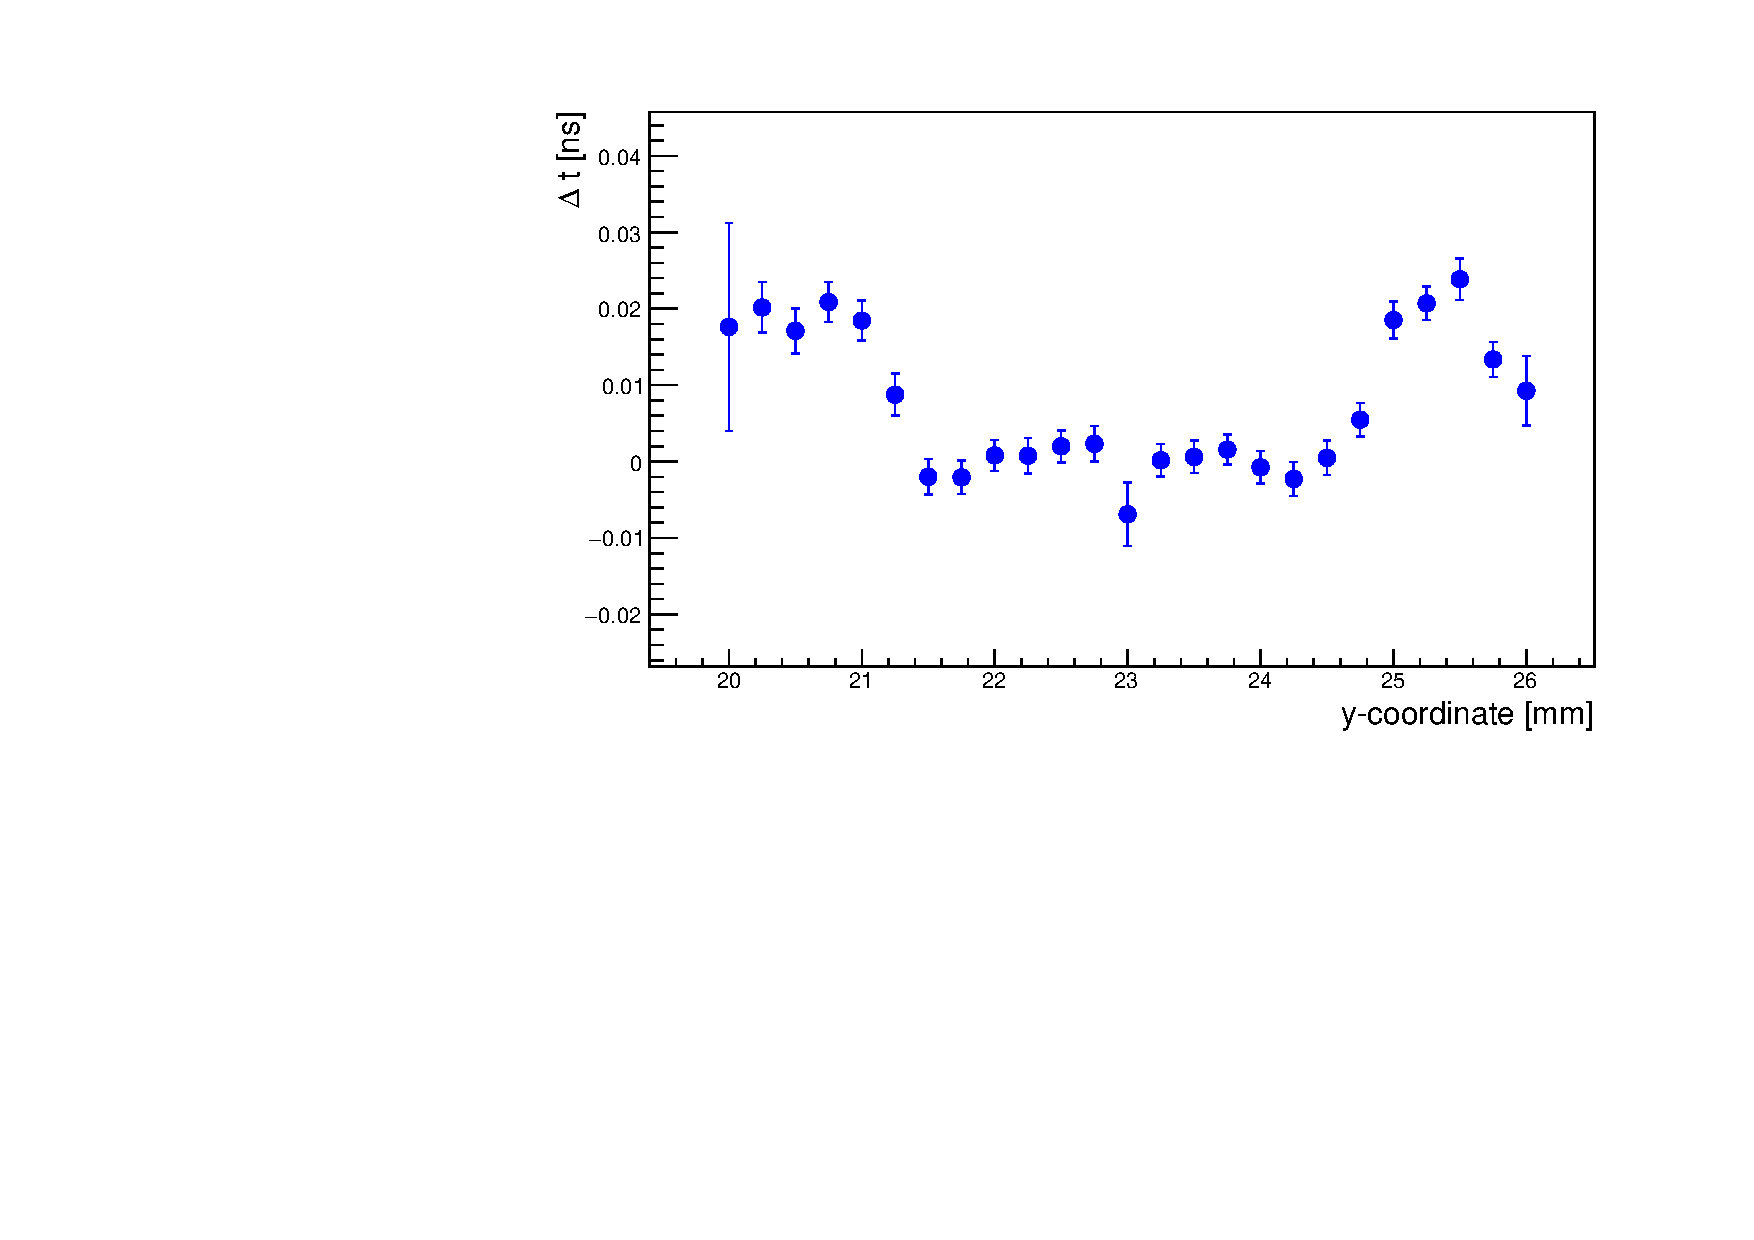
\includegraphics[width=0.48\textwidth]{figs/FNALBoard_HPK50DPix_Run847-891/MeanTime_vs_Y_Ch3_4.pdf} 
\caption{$\Delta t$ measurement across the X- and Y-axes of the HPK 50D-PIX sensor mounted on the FNAL board. The scan of pixels 1 and 2 along the X-axis, and pixels 1 and 3 along the Y-axis is shown, and pixel numberng scheme is defined in Fig.~\ref{fig:HPK_Sensors}.} 
\label{fig:FNAL_HPK50_DTXY} 
\end{figure} 

The measurement of the time resolution scan across the sensor is shown in
Fig.~\ref{fig:FNAL_HPK50_SigmaTXY}. The $\Delta t$ distribution between LGAD
sensor and the Photek 240 MCP-PMT sensor is fitted with a Gaus function, and its
spread $\sigma$ is referred to in the following as the time resolution. We
observe a uniform time resolution around 40~psec across the whole sensor area. 

\begin{figure}[htbp] 
\centering
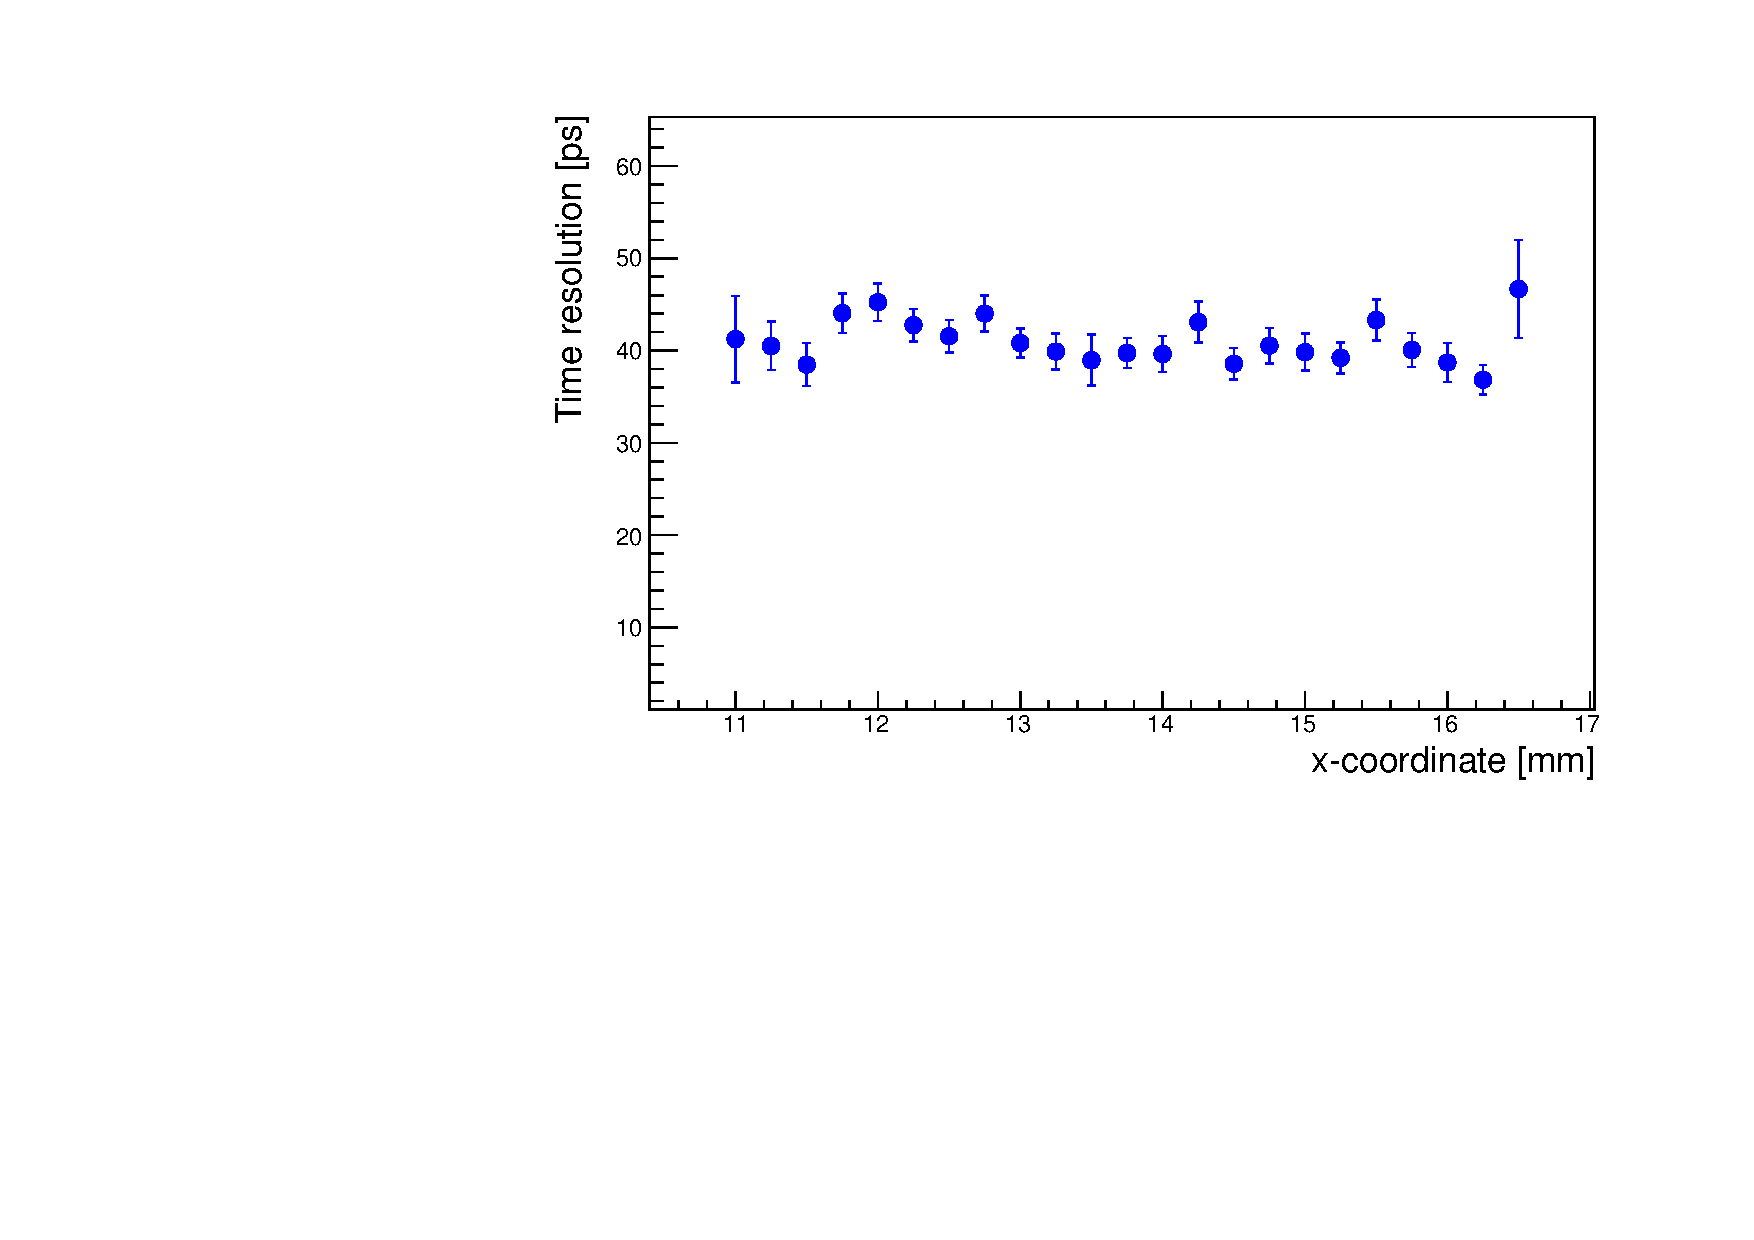
\includegraphics[width=0.48\textwidth]{figs/FNALBoard_HPK50DPix_Run847-891/TimeResolution_vs_X_Ch4_5.pdf} 
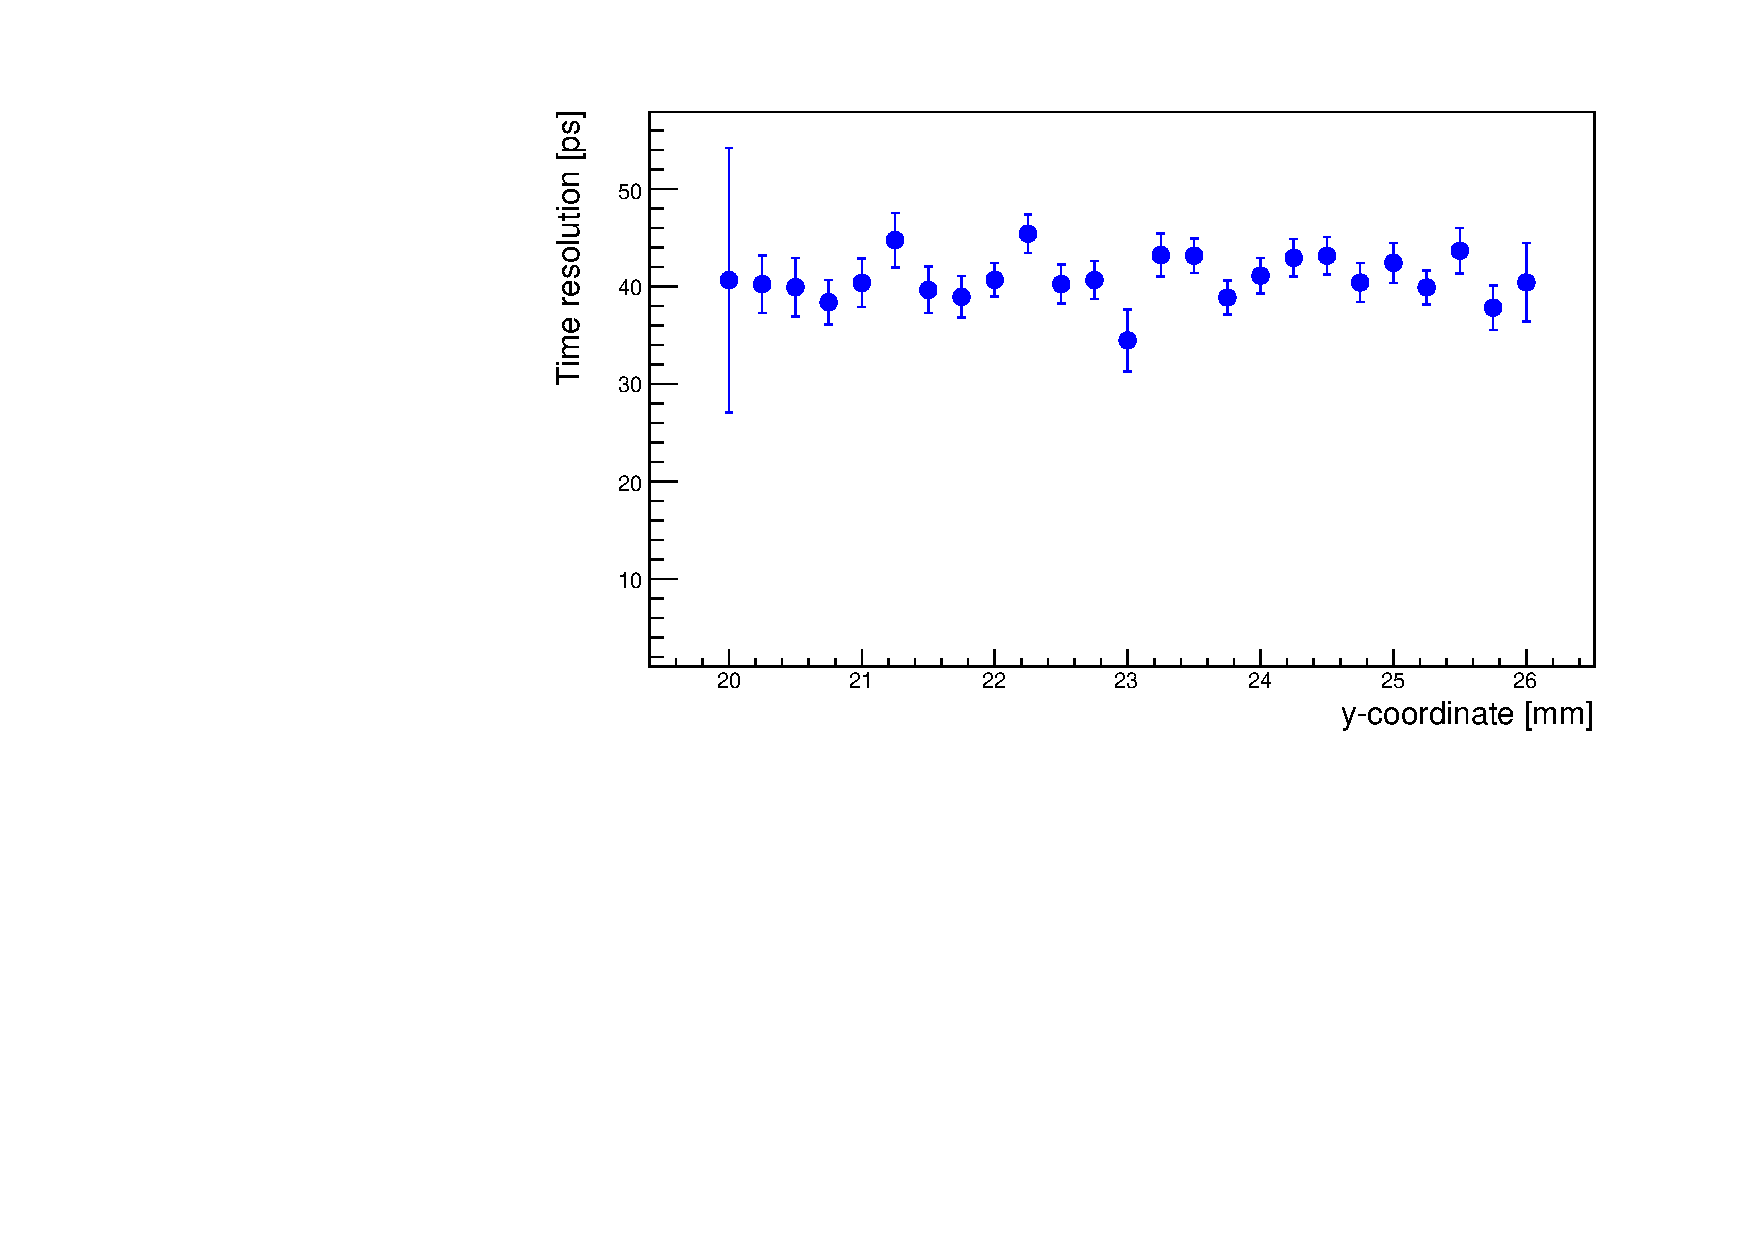
\includegraphics[width=0.48\textwidth]{figs/FNALBoard_HPK50DPix_Run847-891/TimeResolution_vs_Y_Ch3_4.pdf} 
\caption{Time resolution measurement across the X- and Y-axes of the HPK 50D-PIX sensor mounted on the FNAL board. The scan of pixels 1 and 2 along the X-axis, and pixels 1 and 3 along the Y-axis is shown, and pixel numberng scheme is defined in Fig.~\ref{fig:HPK_Sensors}.} 
\label{fig:FNAL_HPK50_SigmaTXY} 
\end{figure} 


%\subsection{Comparison of the boards}


\subsection{Comparison of HPK doping profiles}

KU boards only, ABCD, time resolution, DeltaT, and MPV plots. 

\begin{figure}[htbp] 
\centering
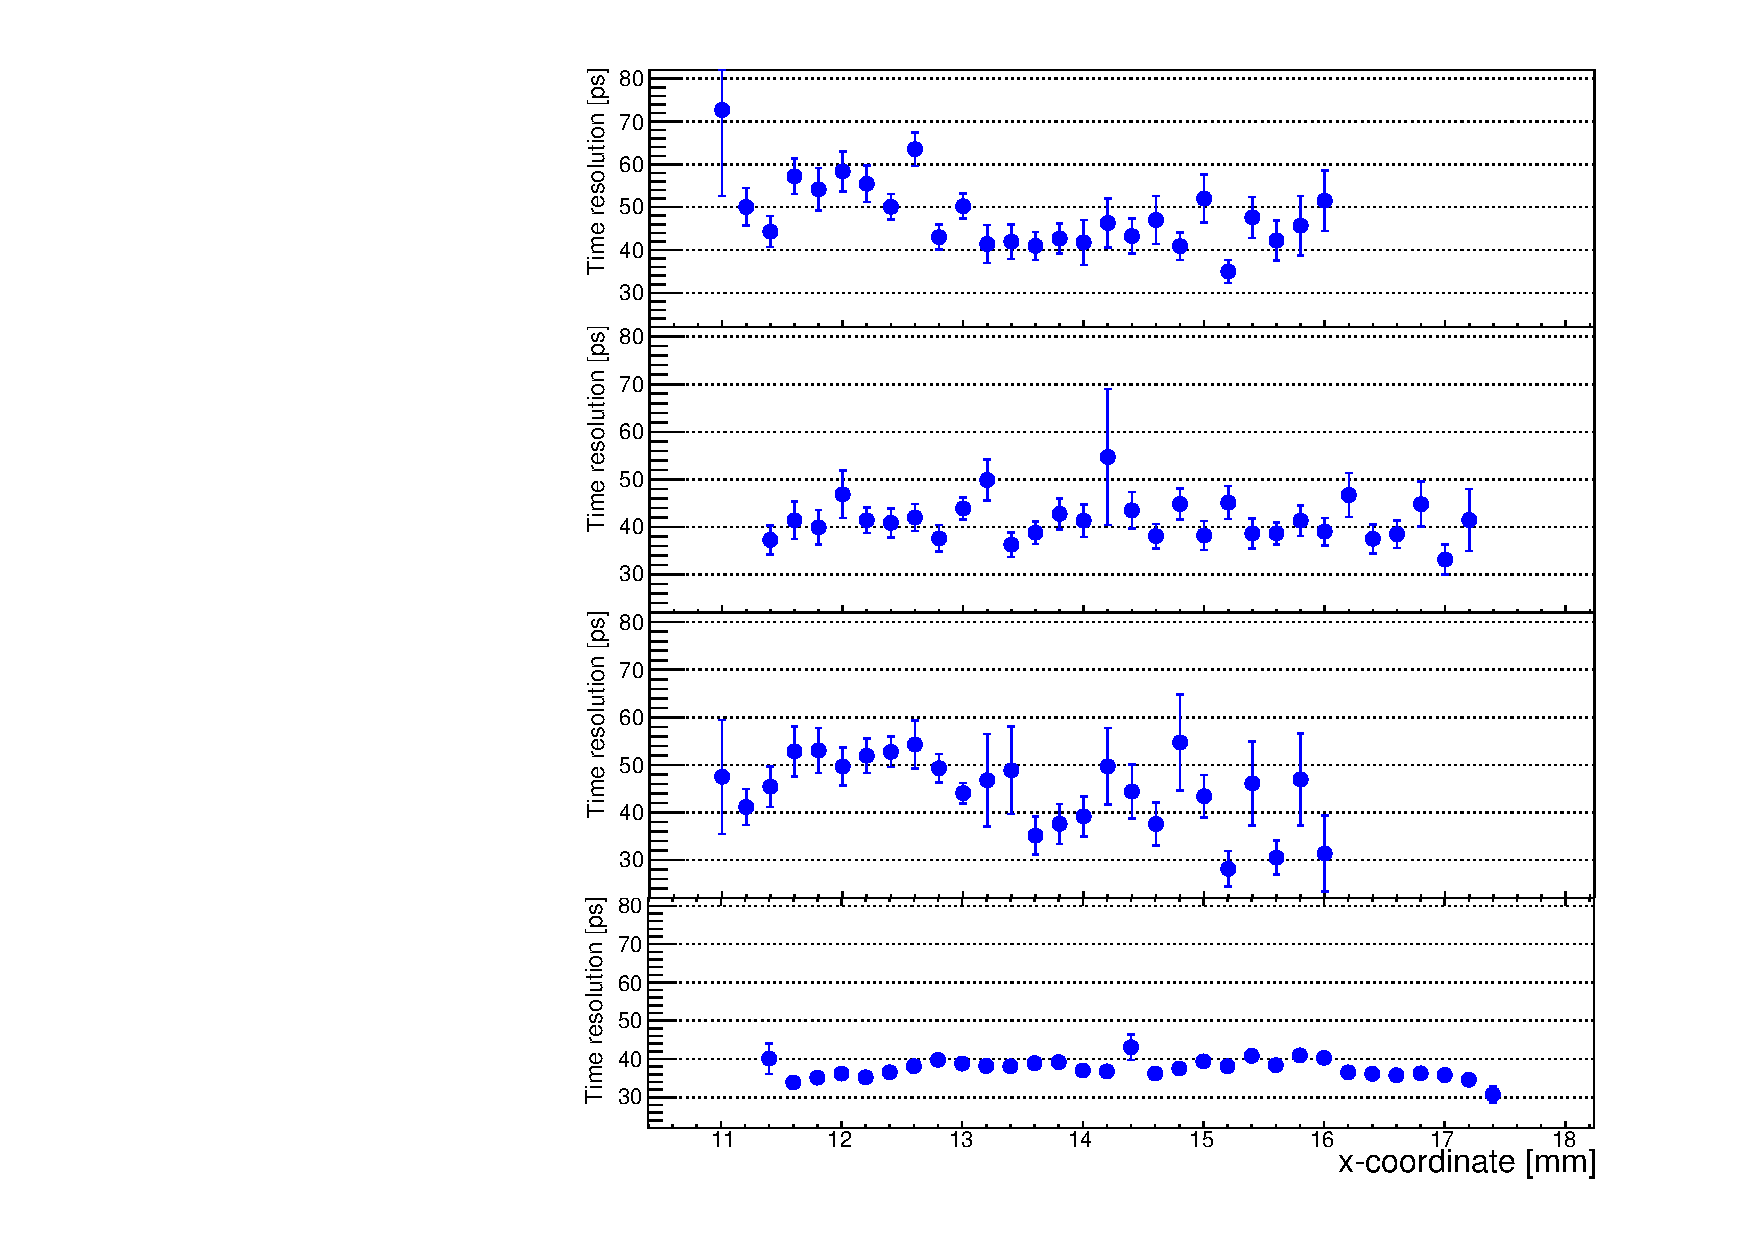
\includegraphics[width=0.9\textwidth]{figs/KUBoard_HPK50ABCD/KUBoard_50ABCD_TimeResolution.pdf} 
\caption{Time resolution on KU board with 50A, B, C, D } 
\label{fig:Sensors} 
\end{figure} 

\begin{figure}[htbp] 
\centering
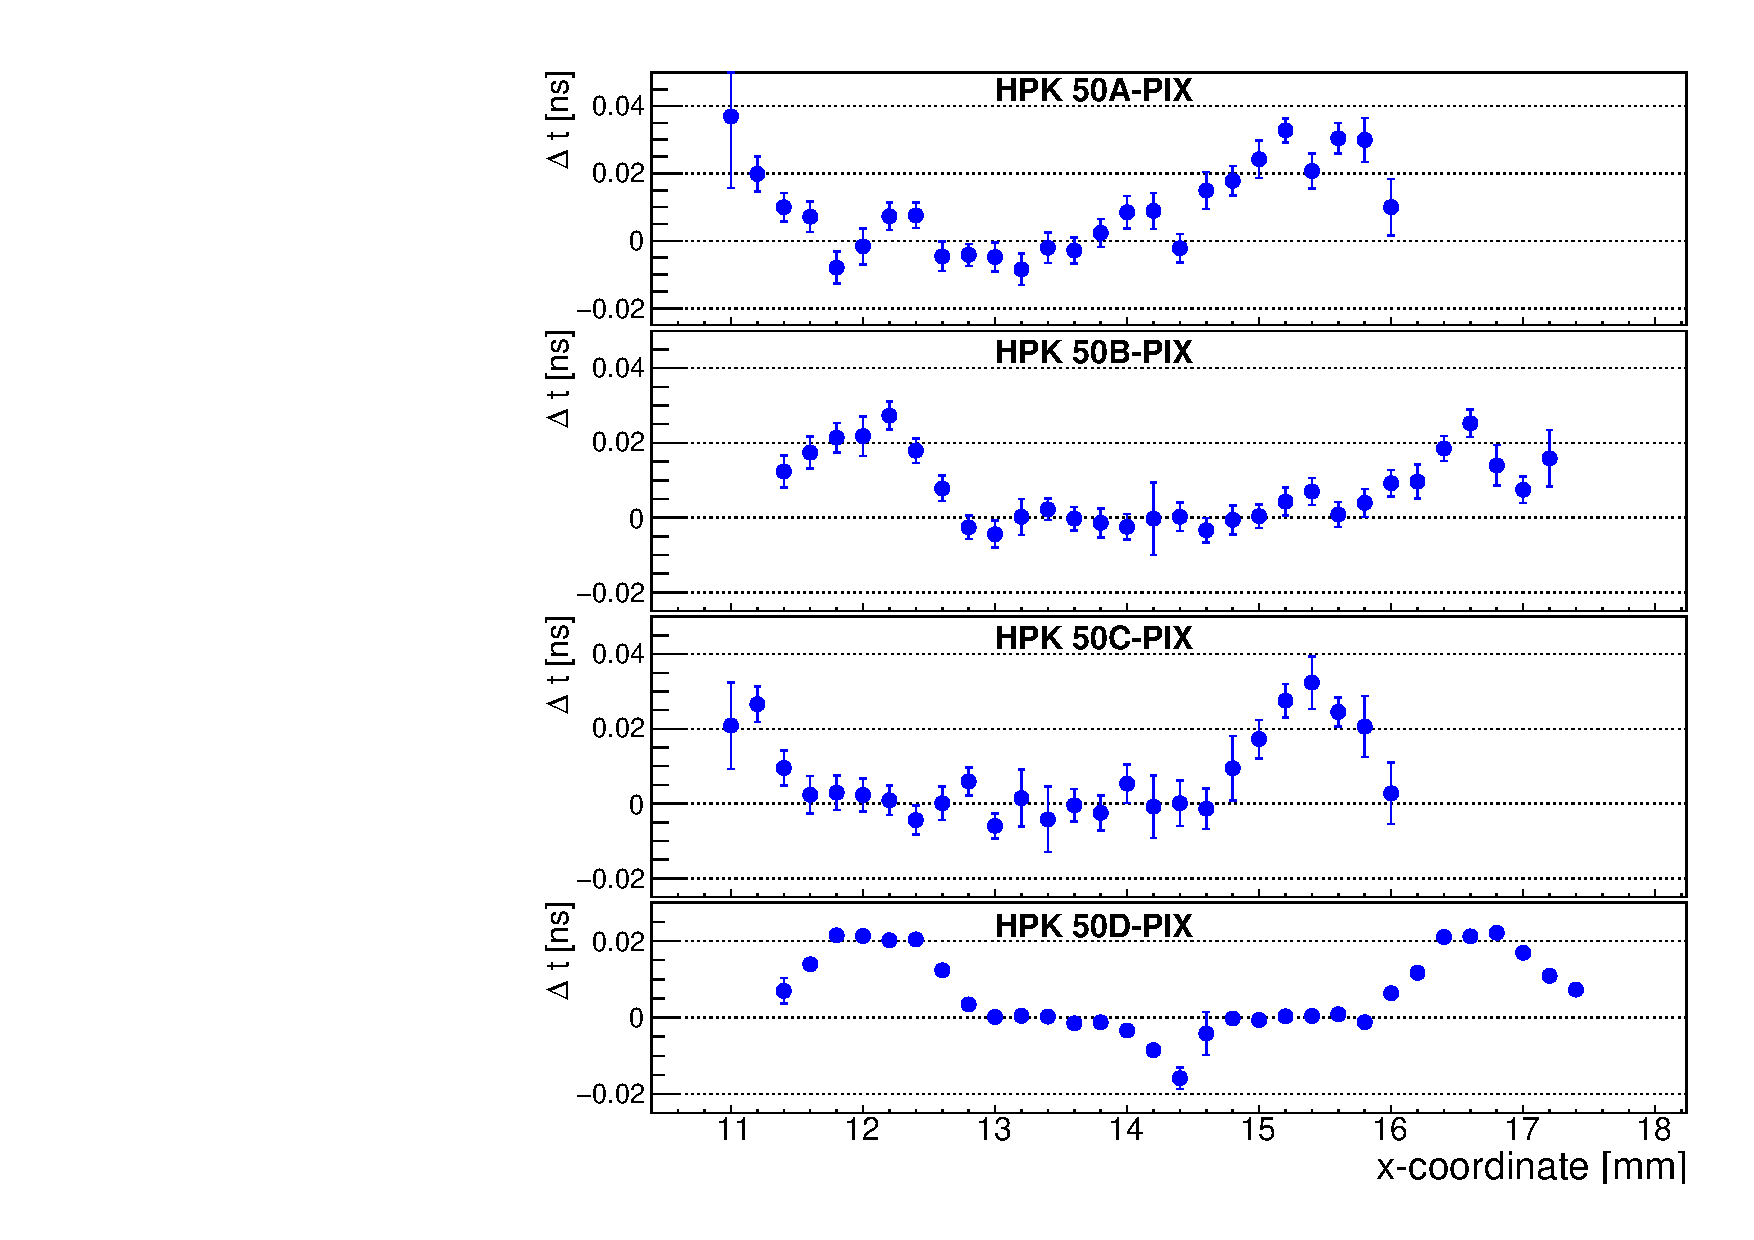
\includegraphics[width=0.9\textwidth]{figs/KUBoard_HPK50ABCD/KUBoard_50ABCD_MeanTime.pdf} 
\caption{DeltaT on KU board with 50A, B, C, D } 
\label{fig:Sensors} 
\end{figure} 

\begin{figure}[htbp] 
\centering
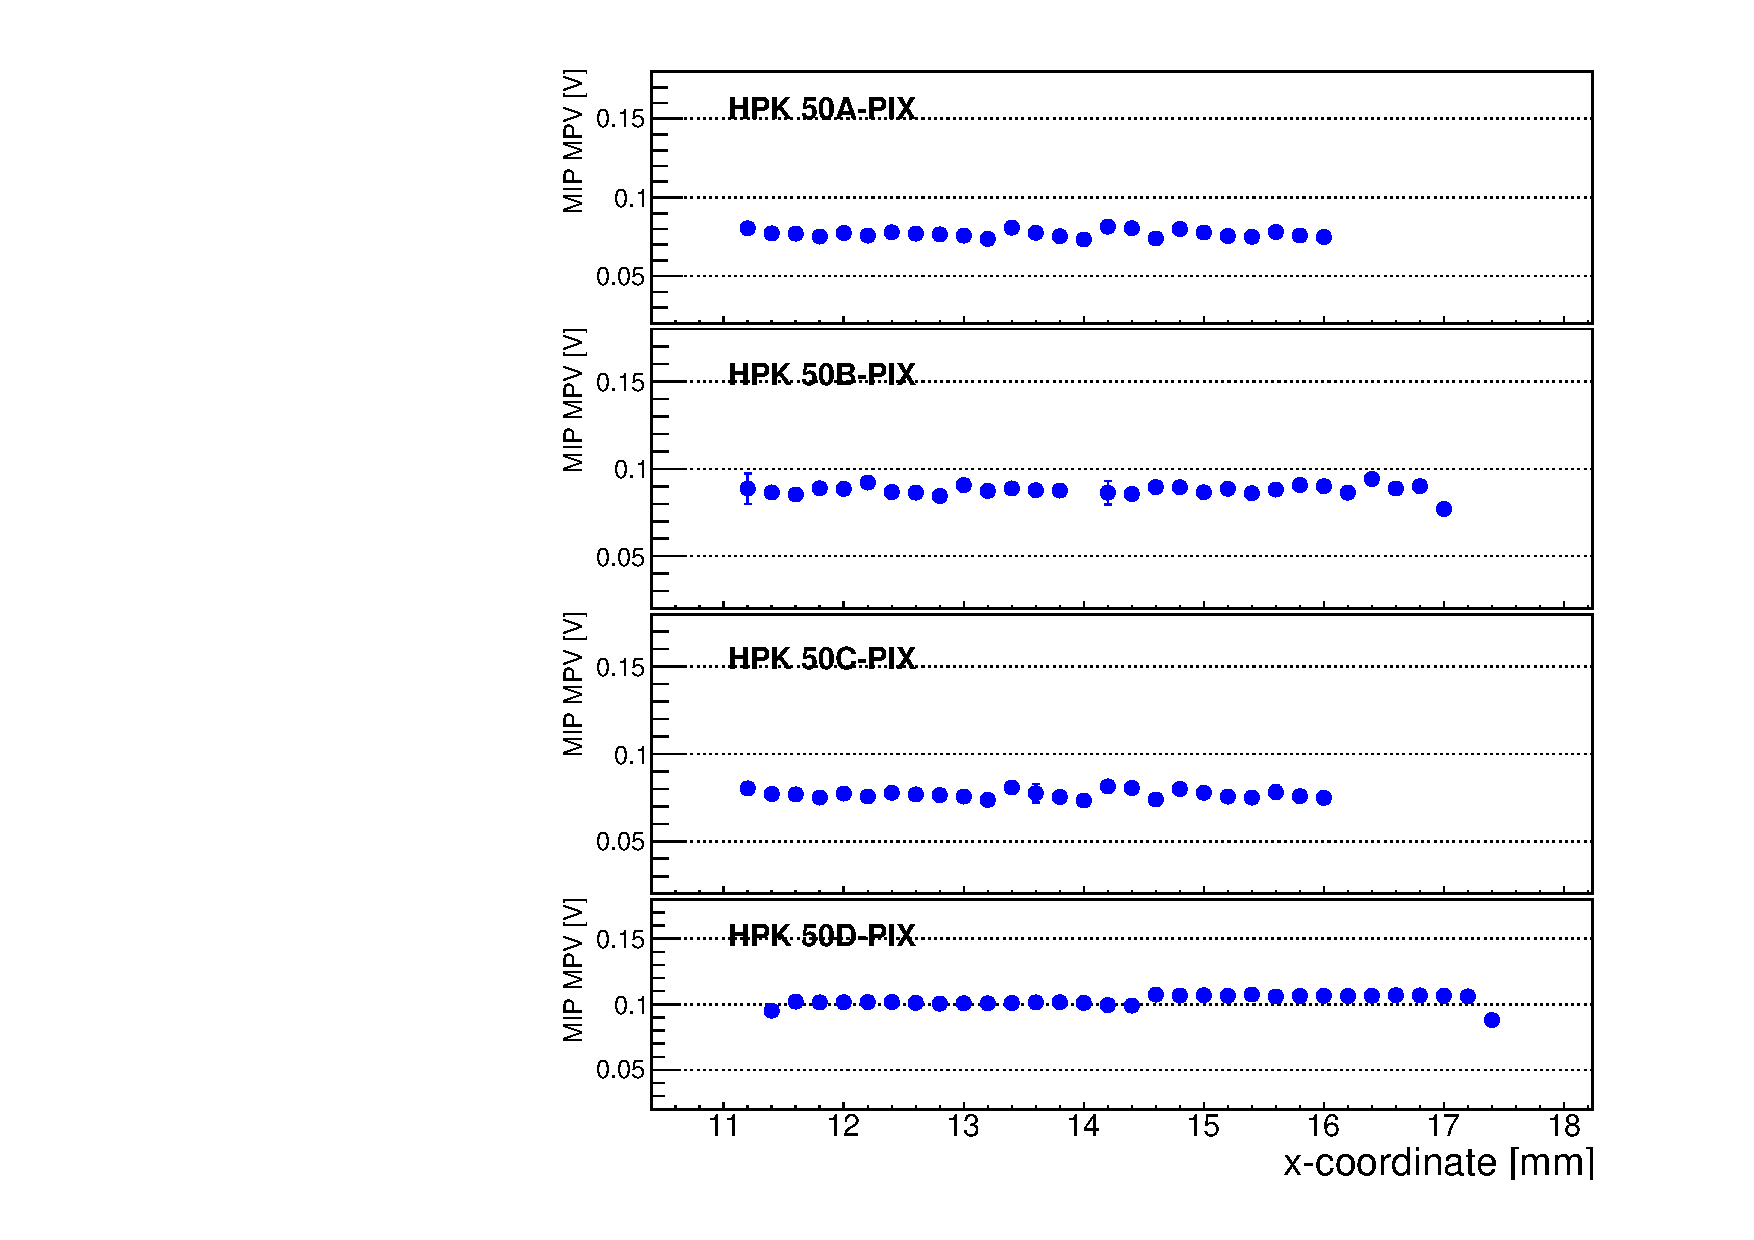
\includegraphics[width=0.9\textwidth]{figs/KUBoard_HPK50ABCD/KUBoard_50ABCD_MPV.pdf} 
\caption{MPV on KU board with 50A, B, C, D } 
\label{fig:Sensors} 
\end{figure} 



\subsection{Comparison of HPK 50 $\mu$m with 80 $\mu$m}

\begin{figure}[htbp] 
\centering
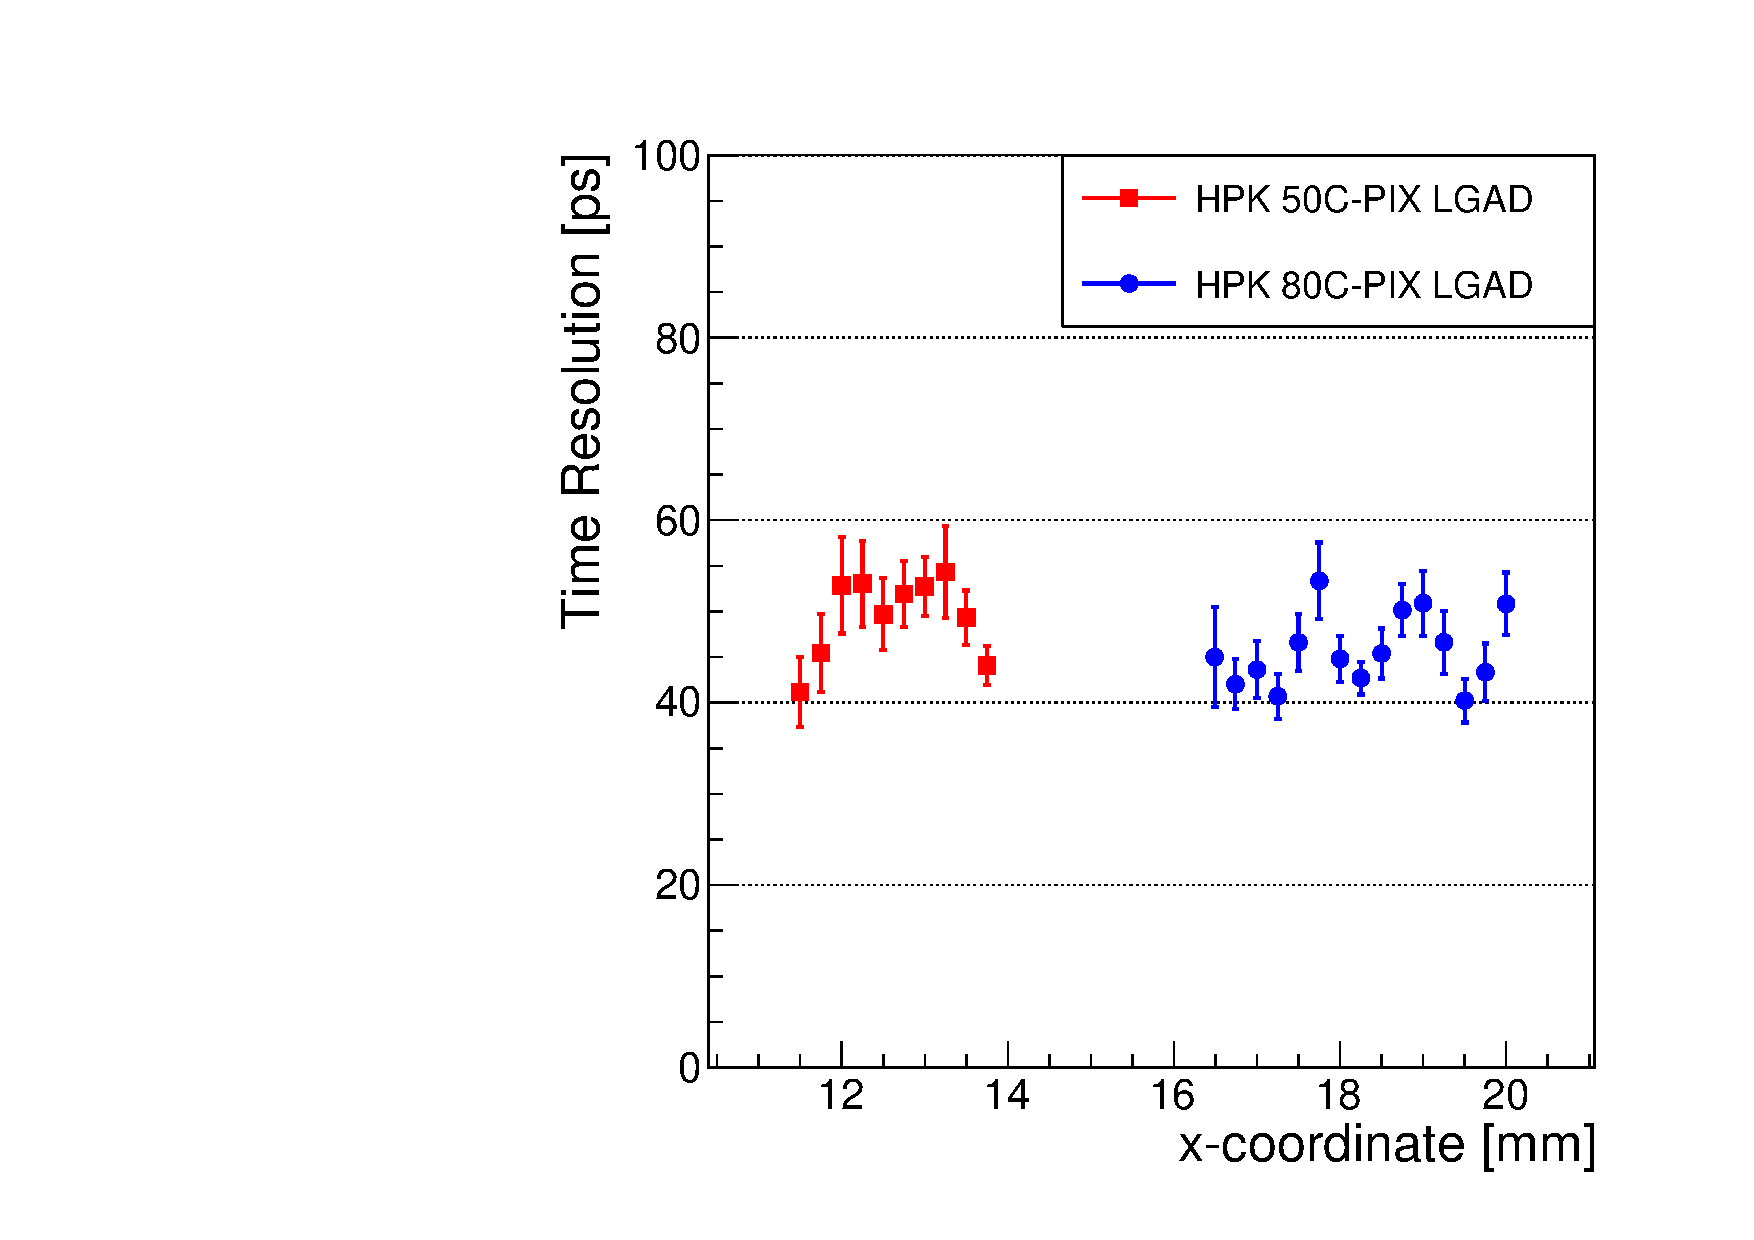
\includegraphics[width=0.7\textwidth]{figs/FNAL_TimeResolution_vs_X_HPK50CVs80C.pdf} 
\caption{Comparison of time resolution in FNAL 80C versus KU 50C sensors } 
\label{fig:Sensors} 
\end{figure} 


\subsection{Temperature dependence of the LGAD sensors}

\begin{figure}[htbp] 
\centering
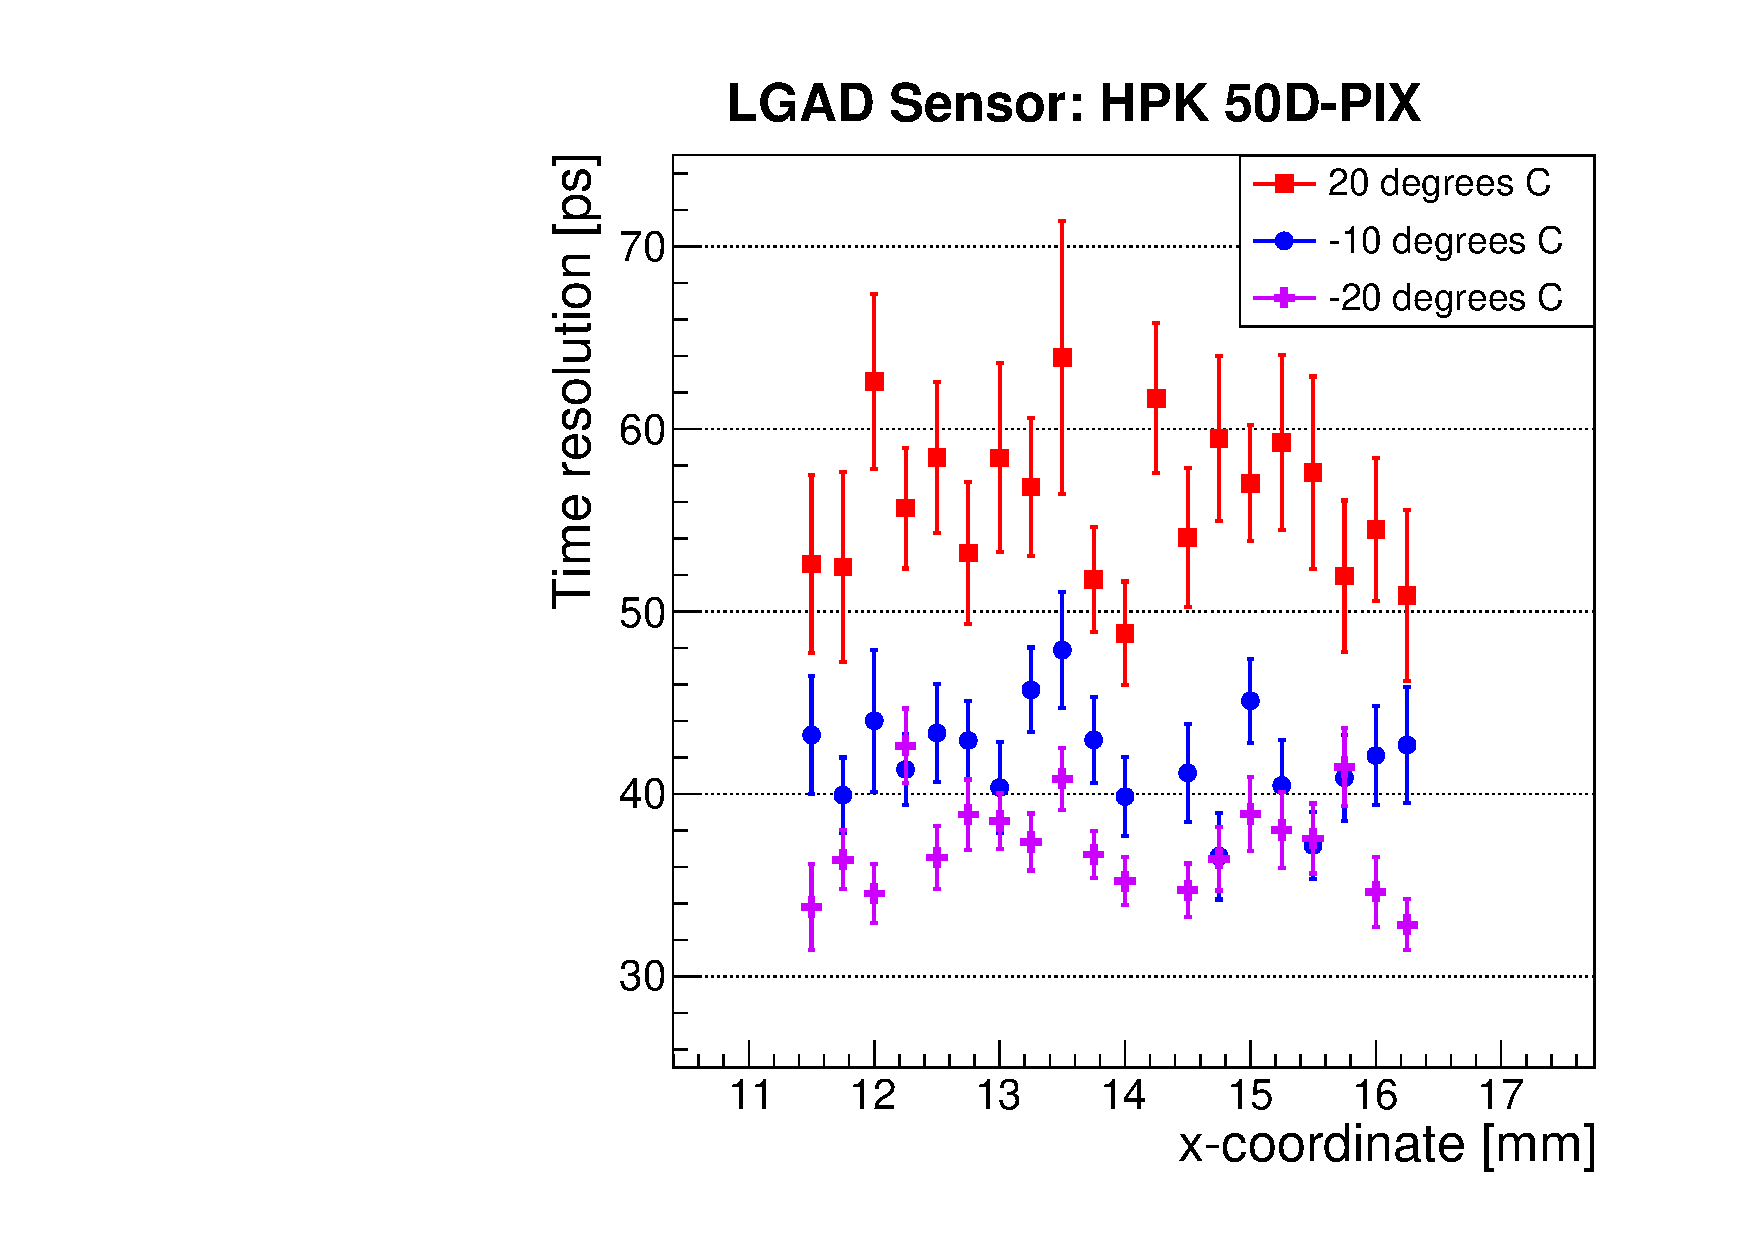
\includegraphics[width=0.9\textwidth]{figs/FNAL_TimeResolution_vs_X_HPK50D_TemperatureDependance.pdf} 
\caption{Time resolution on FNAL board with 50D at +20, -10, -20C} 
\label{fig:Sensors} 
\end{figure} 

\begin{figure}[htbp] 
\centering
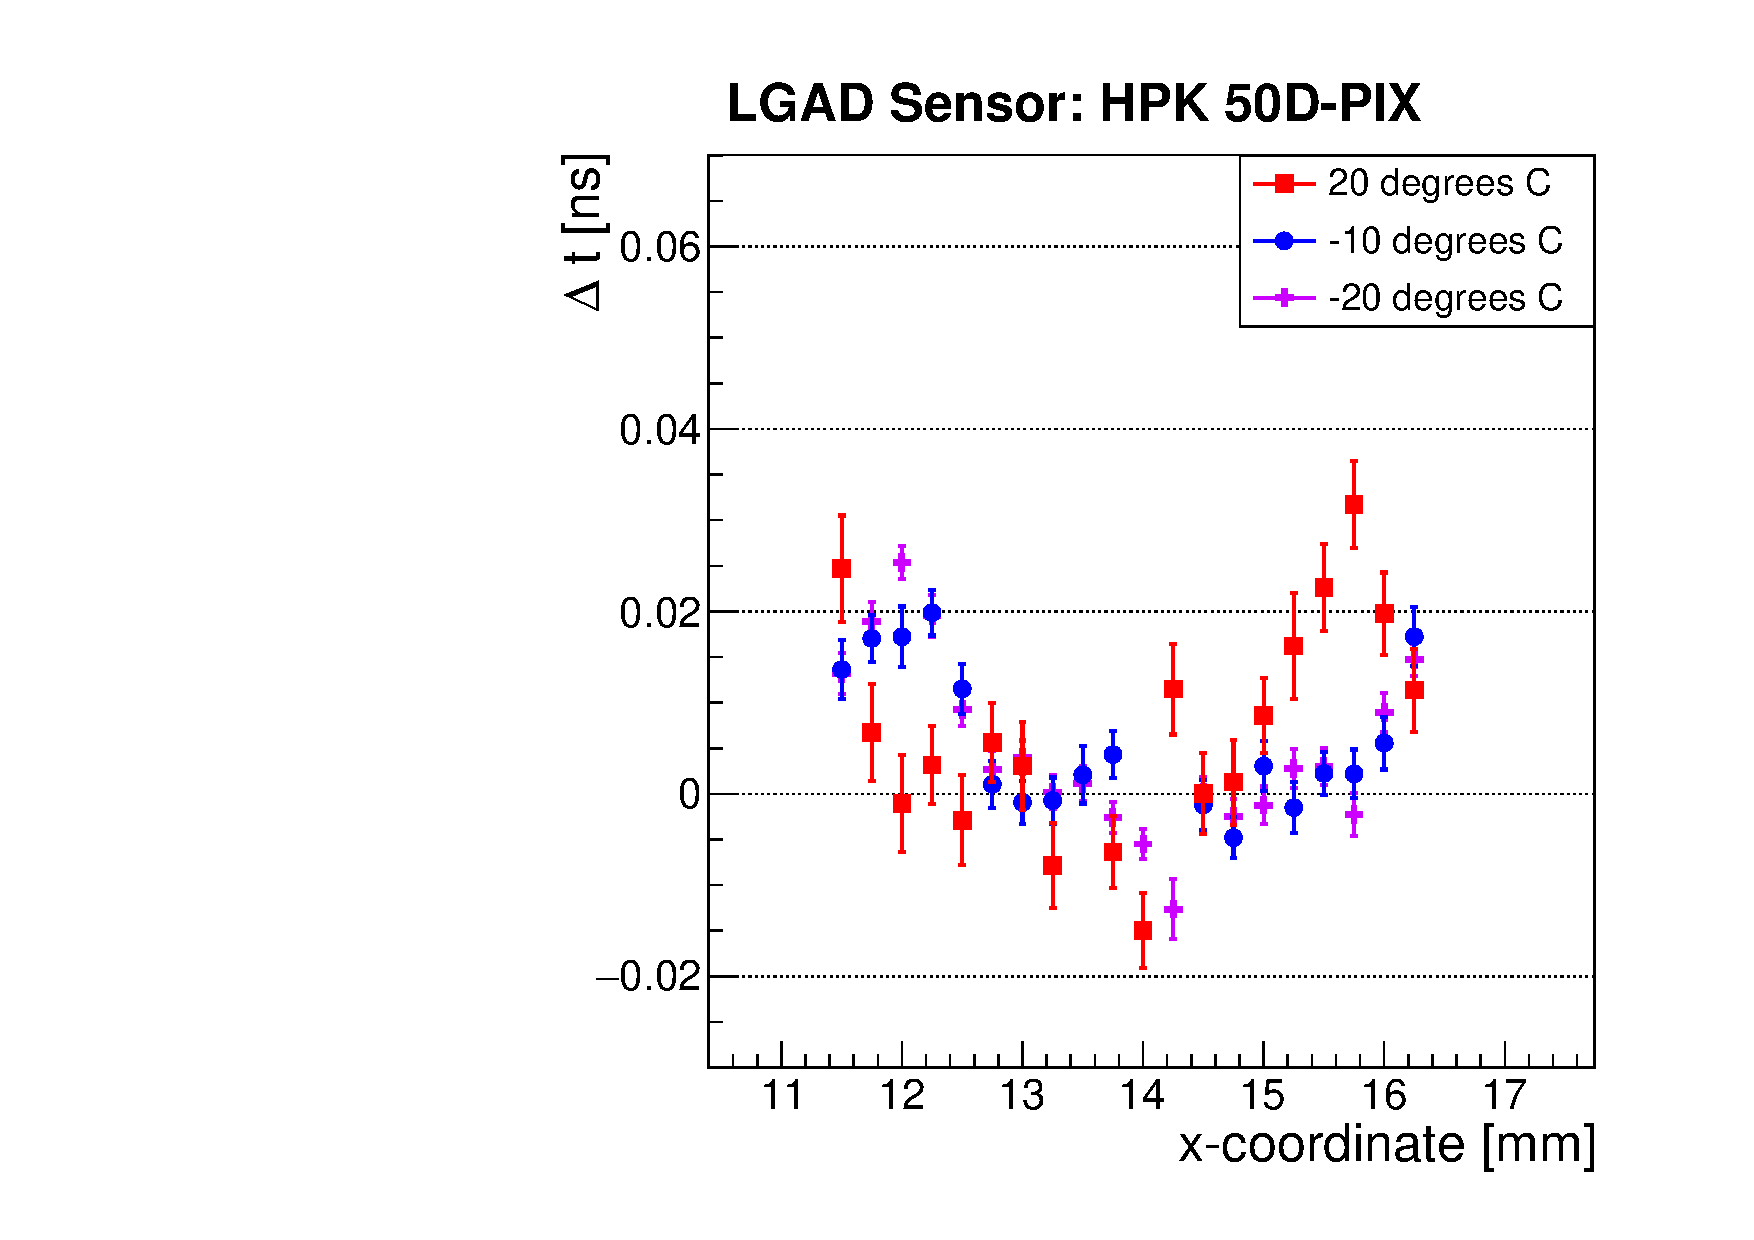
\includegraphics[width=0.9\textwidth]{figs/FNAL_MeanTime_vs_X_HPK50D_TemperatureDependance.pdf} 
\caption{DeltaT on FNAL board with 50D at +20, -10, -20C} 
\label{fig:Sensors} 
\end{figure} 


\begin{figure}[htbp] 
\centering
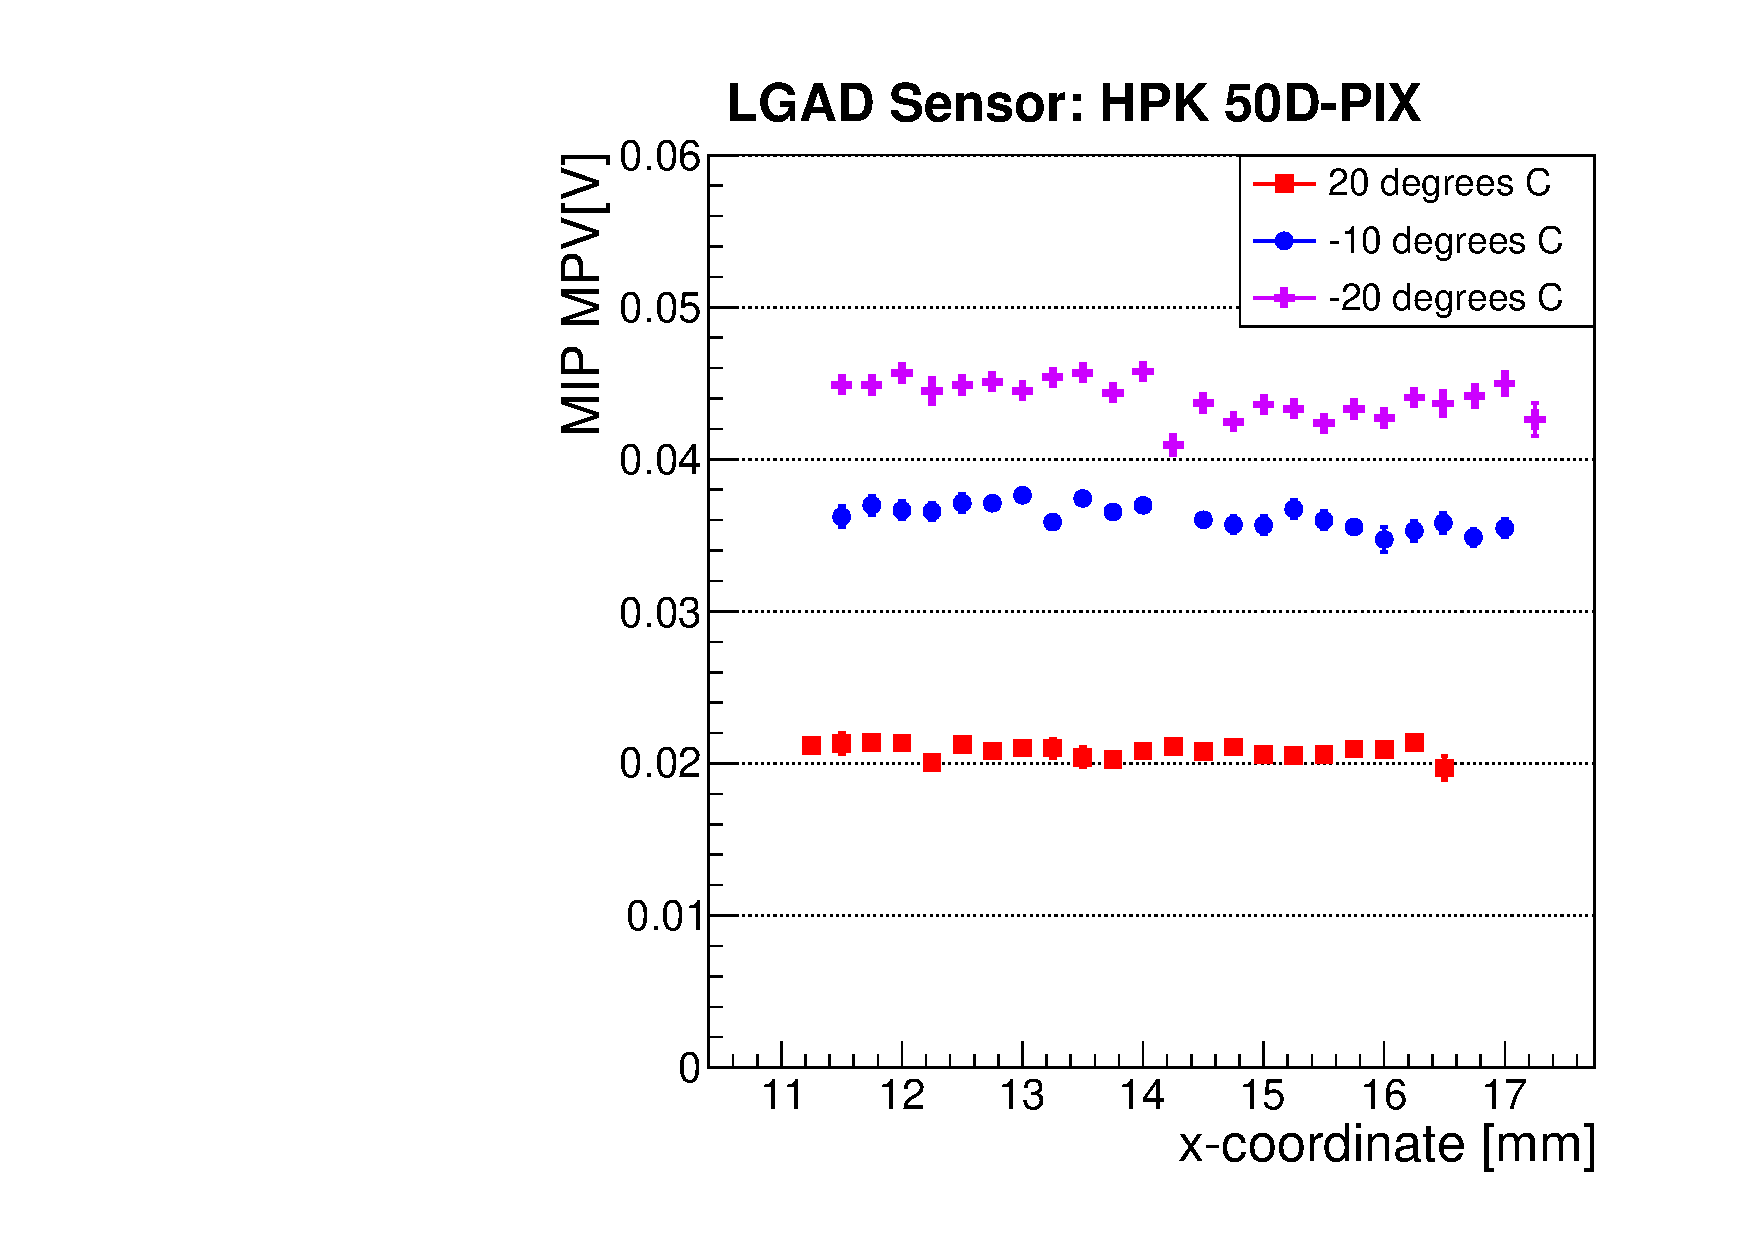
\includegraphics[width=0.9\textwidth]{figs/FNAL_MPV_vs_X_HPK50D_TemperatureDependance.pdf} 
\caption{MPV on FNAL board with 50D at +20, -10, -20C} 
\label{fig:Sensors} 
\end{figure} 

\subsection{Radiation tolerance of the LGADs up to 6$\times 10^{14}$}

\begin{figure}[htbp] 
\centering
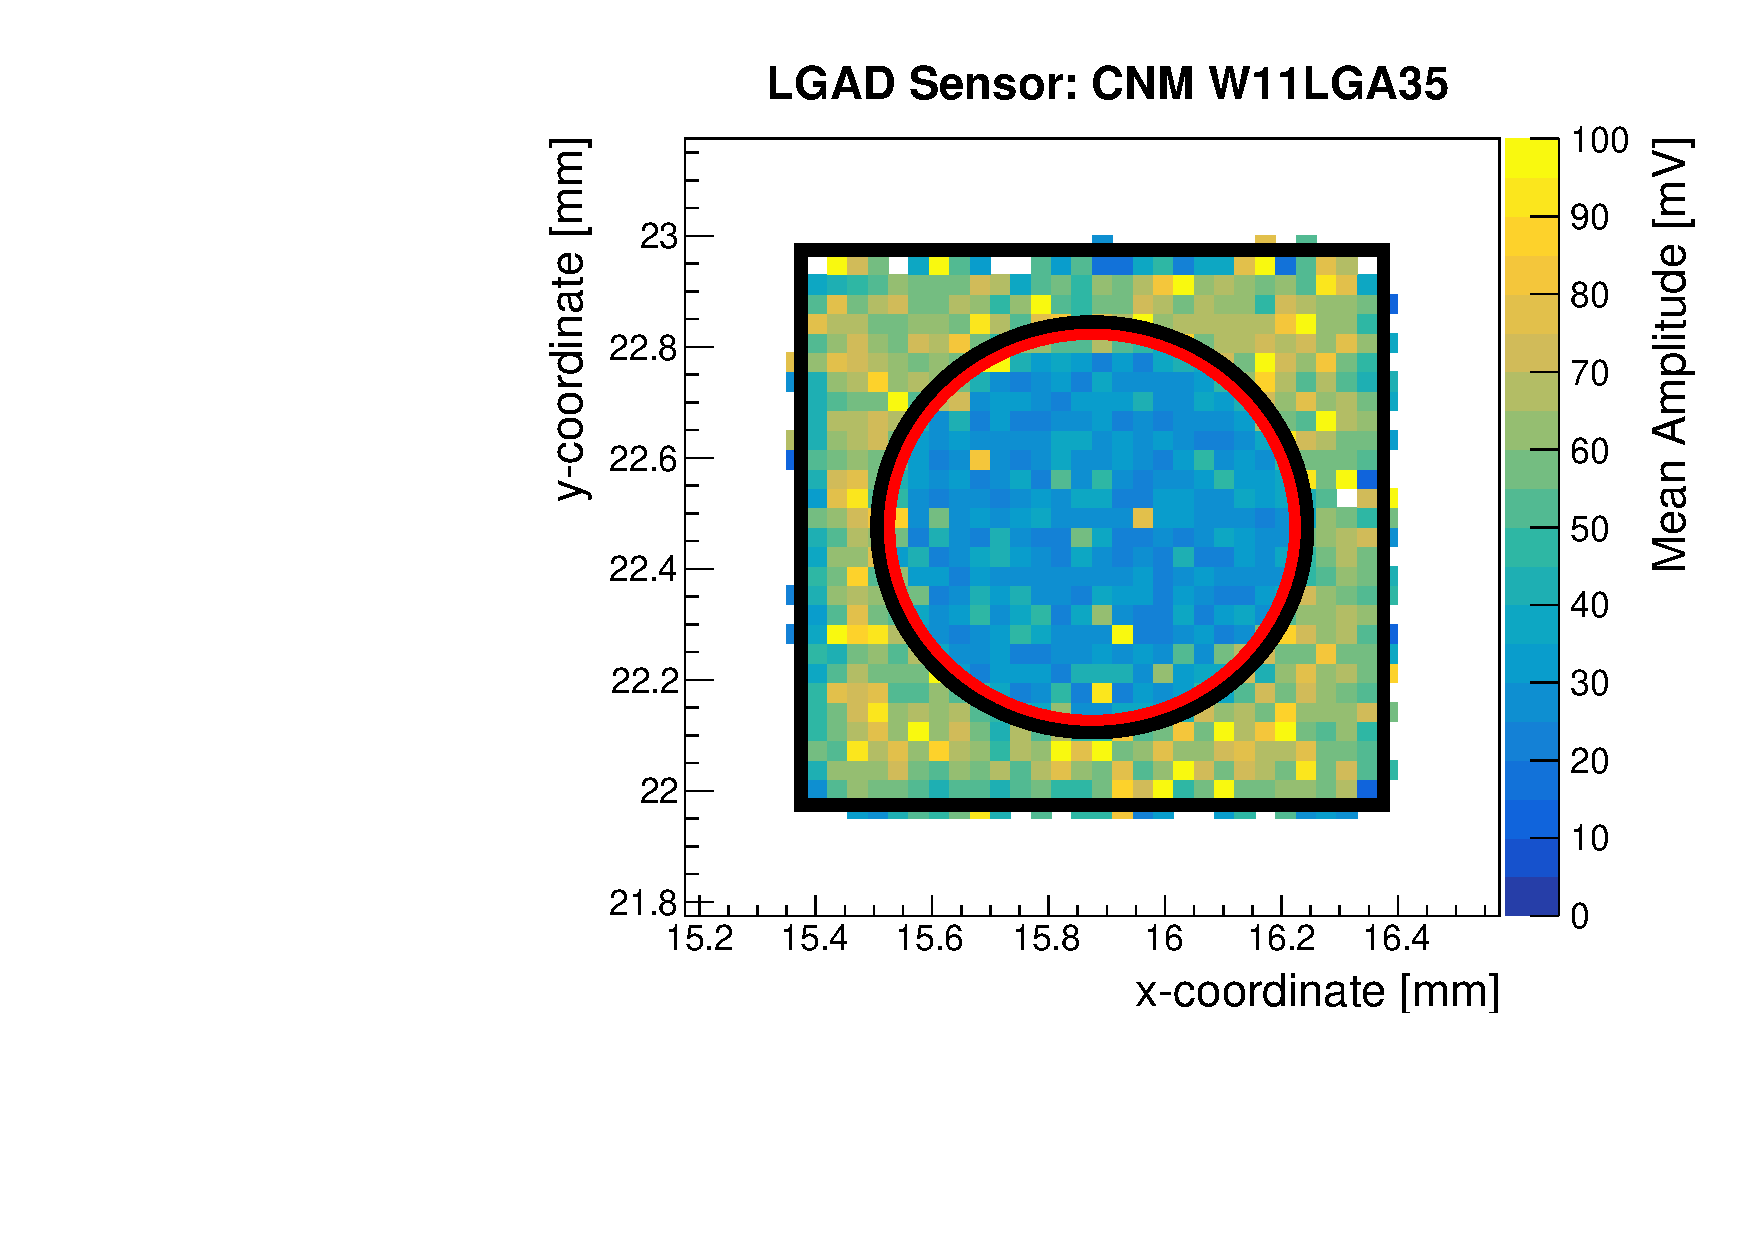
\includegraphics[width=0.48\textwidth]{figs/USCSBoard_HPK50DIrradiated-CNMW11LGA35_Run936-961/CNM_irradiated_amp_Map.pdf} \hfill
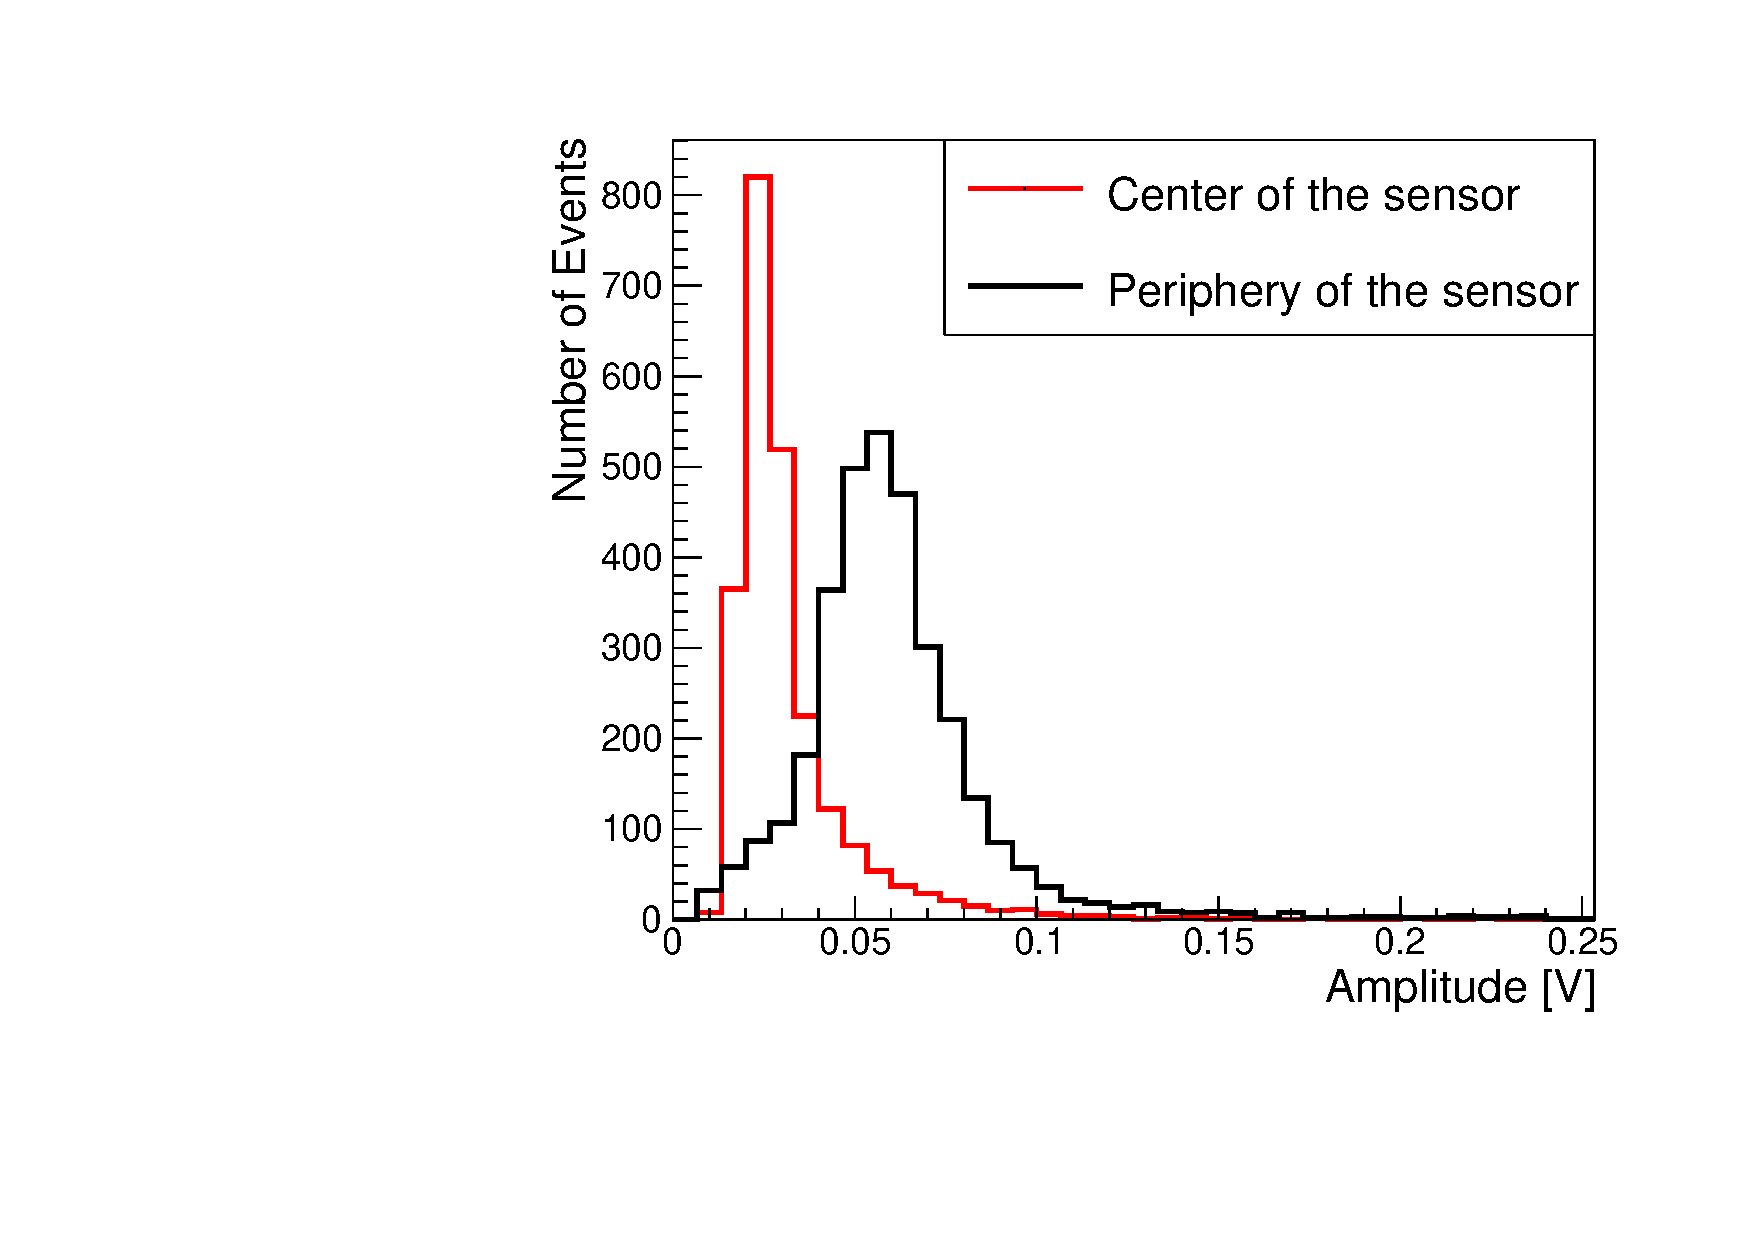
\includegraphics[width=0.48\textwidth]{figs/USCSBoard_HPK50DIrradiated-CNMW11LGA35_Run936-961/CNM_irradiated_amp_1D.pdf} 
\caption{(Left) The map of the amplitude distribution on the irradiated CNM W11LGA35 sensor across X and Y coordinates. Two distinct regions on the sensor surface can be identified according to the amplitude distribution: the center of the sensor (area within the red circle), and the periphery of the sensor (area between the black circle and black square). (Right) Amplitude distribution in the two areas of the irradiated CNM W11LGA35 sensor.} 
\label{fig:Sensors} 
\end{figure} 

\begin{figure}[htbp] 
\centering
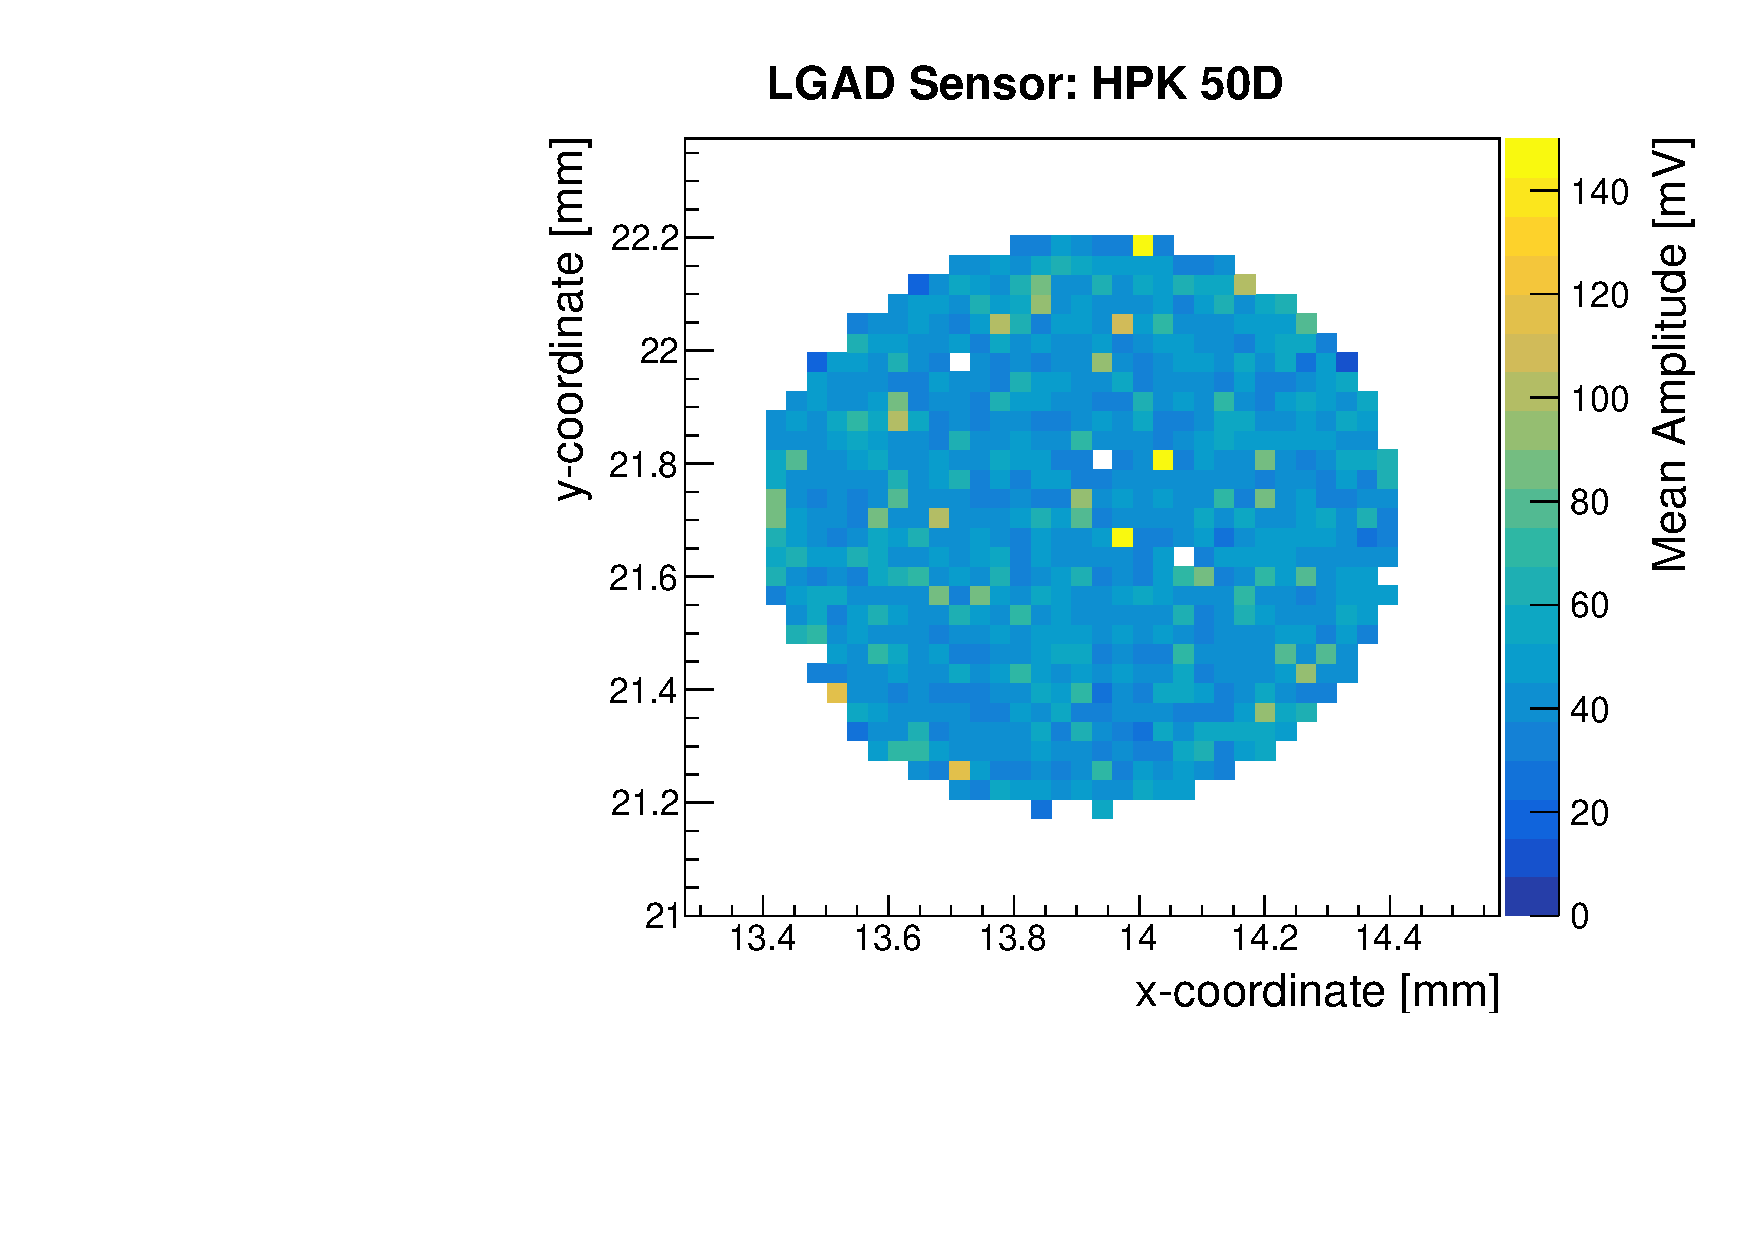
\includegraphics[width=0.48\textwidth]{figs/USCSBoard_HPK50DIrradiated-CNMW11LGA35_Run936-961/HPK_irradiated_amp_Map.pdf} \hfill
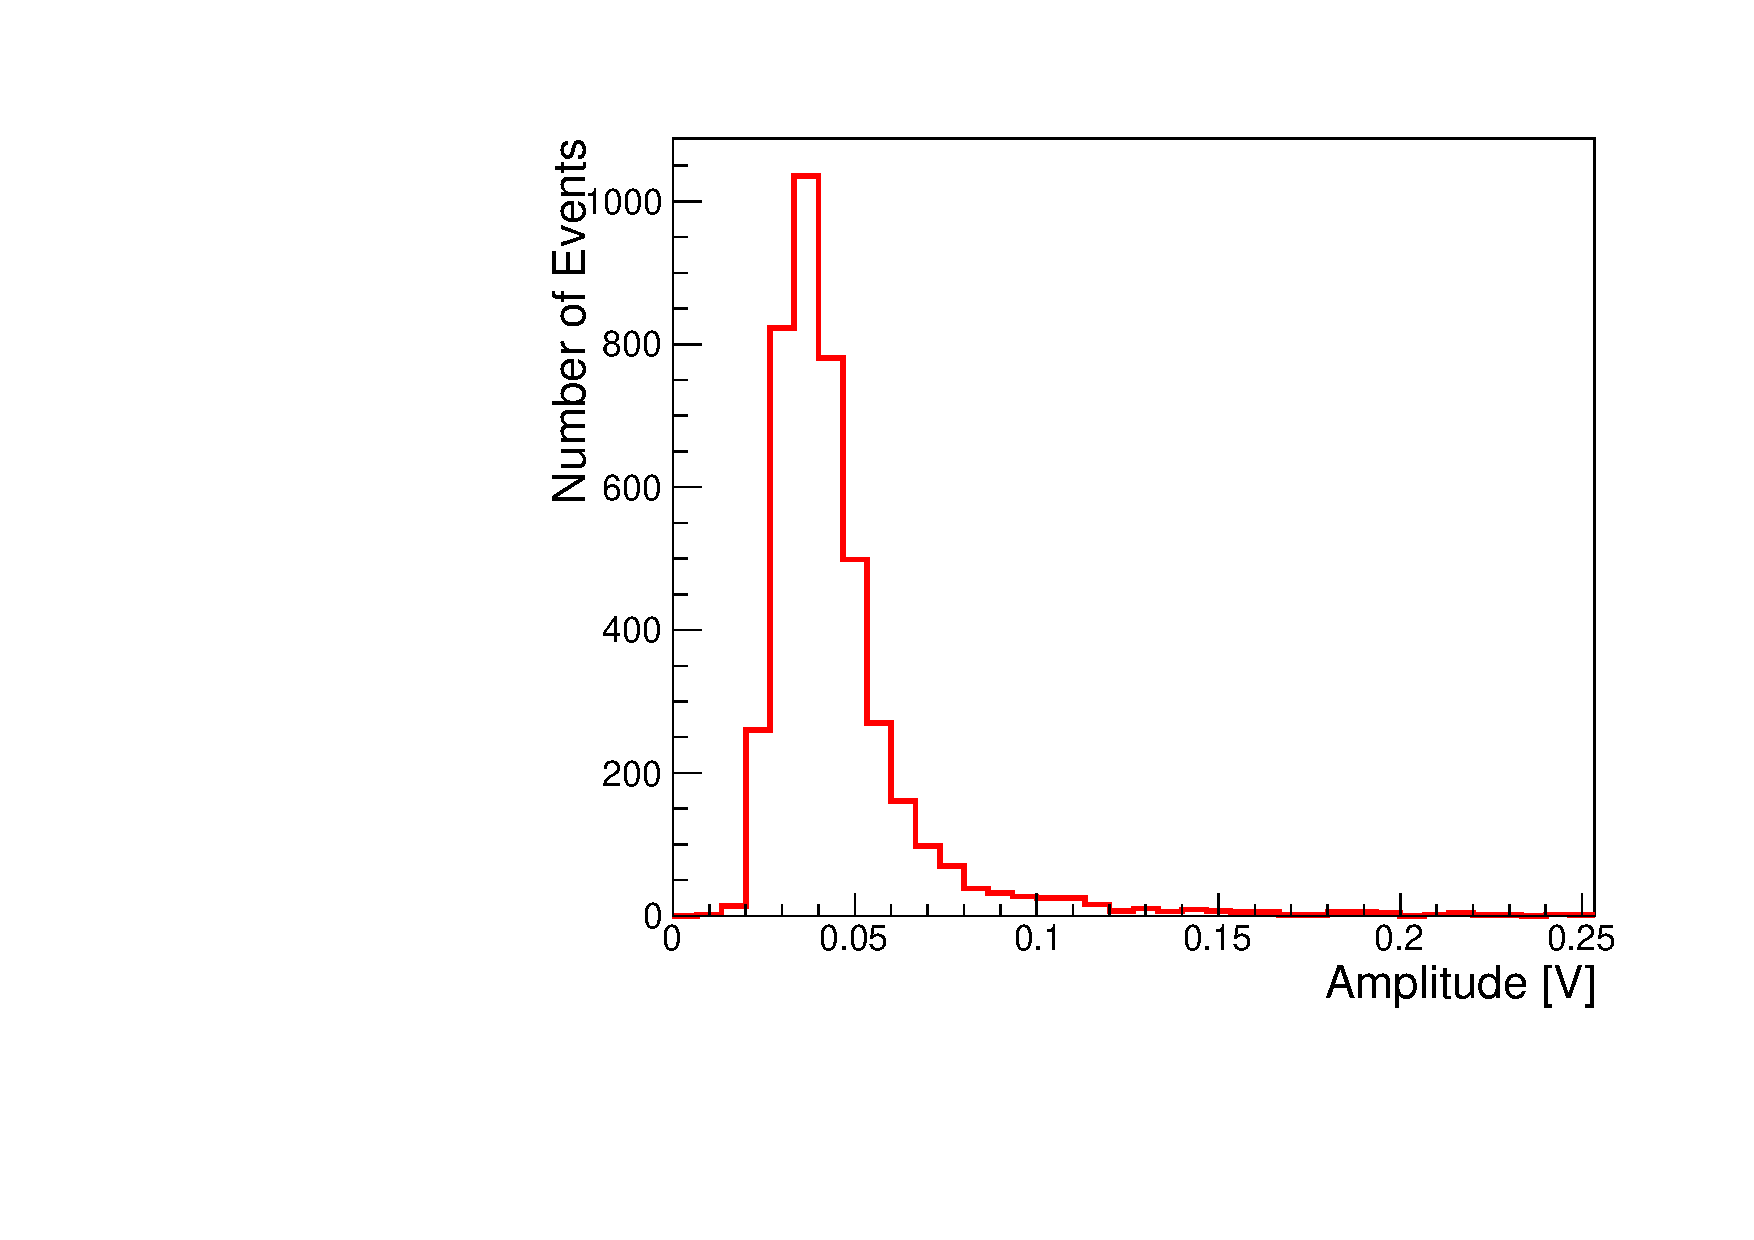
\includegraphics[width=0.48\textwidth]{figs/USCSBoard_HPK50DIrradiated-CNMW11LGA35_Run936-961/HPK_irradiated_amp_1D.pdf} 
\caption{(Left) The map of the amplitude distribution on the irradiated HPK 50D sensor across X and Y coordinates. Two distinct regions on the sensor surface can be identified according to the amplitude distribution: the center of the sensor (area within the red circle), and the periphery of the sensor (area between the black circle and black square). (Right) Amplitude distribution in the two areas of the irradiated HPK 50D sensor.} 
\label{fig:Sensors} 
\end{figure} 

\begin{figure}[htbp] 
\centering
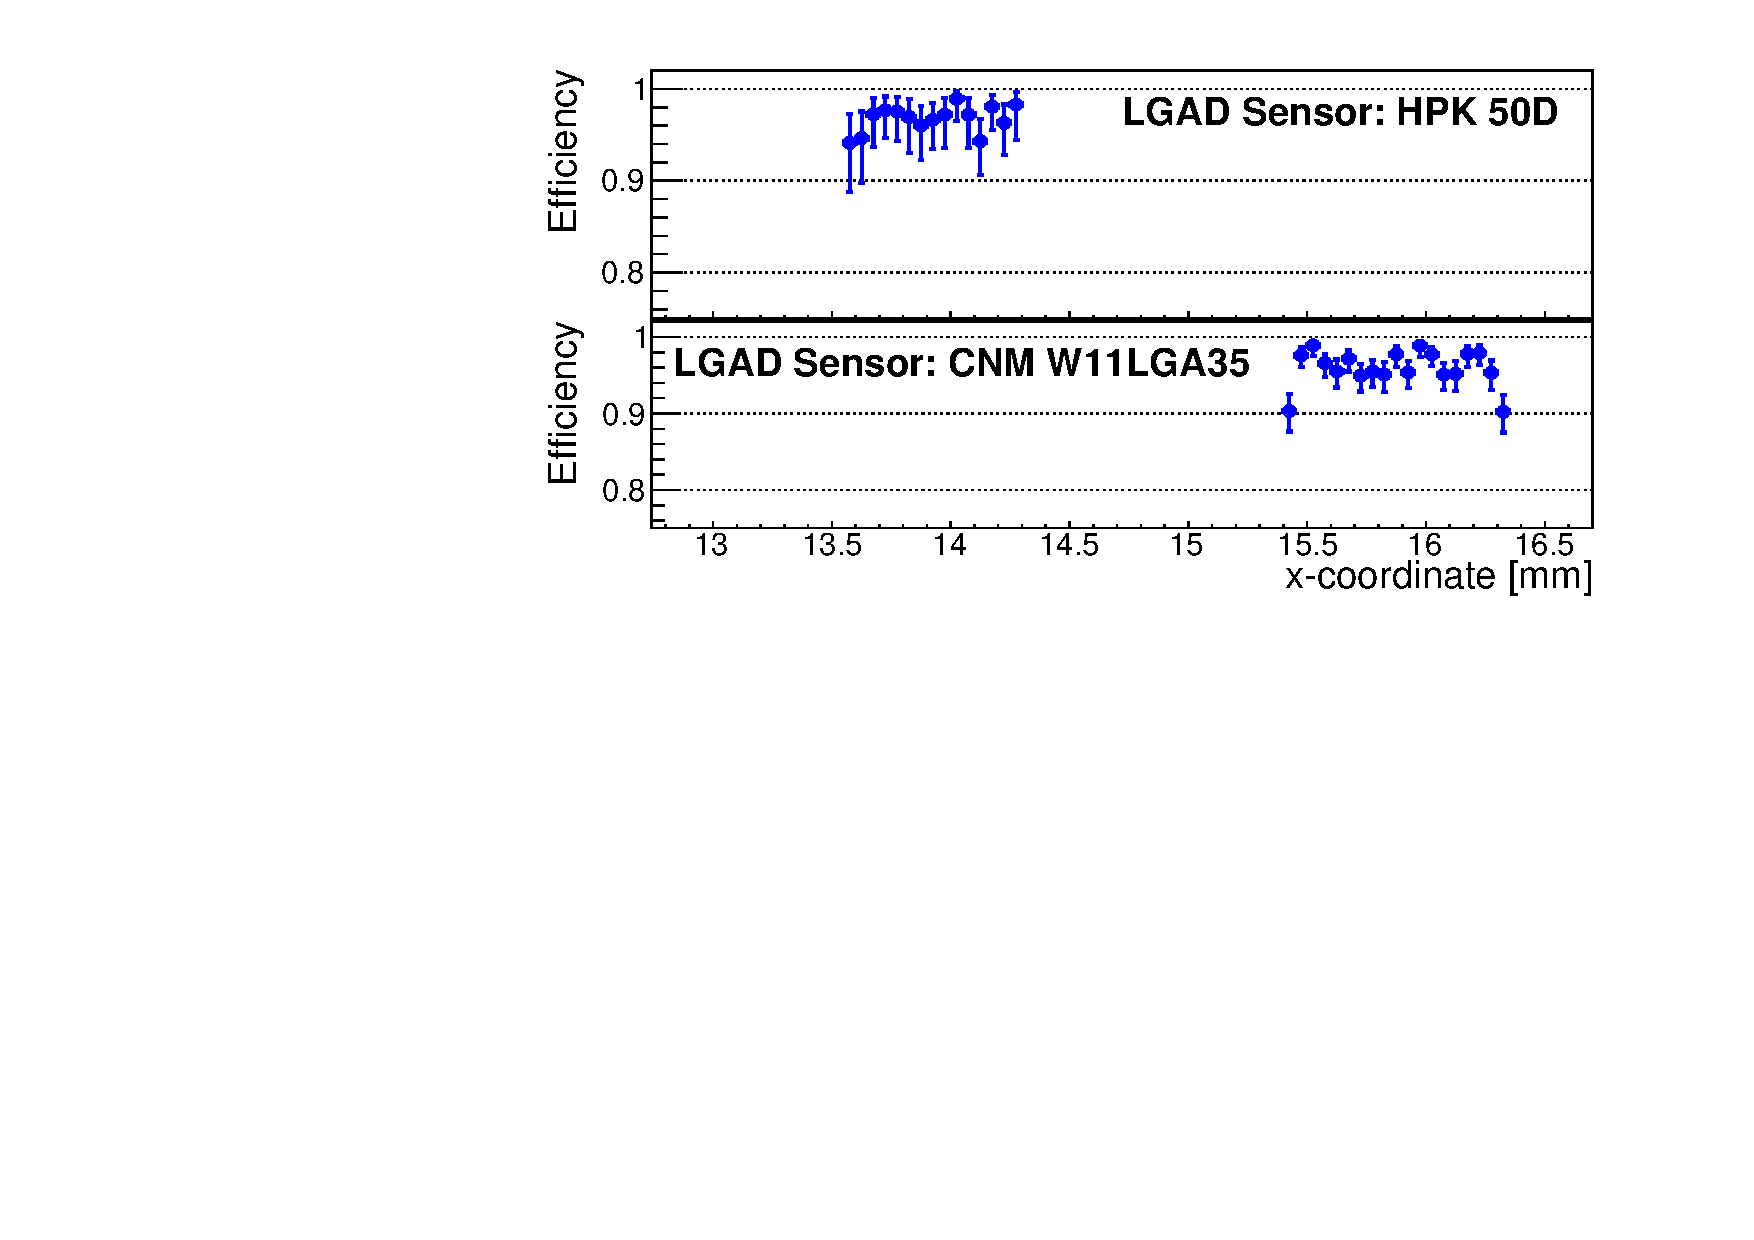
\includegraphics[width=0.90\textwidth]{figs/USCSBoard_HPK50DIrradiated-CNMW11LGA35_Run936-961/IrradiatedSensorStudy_Efficiency_vs_X.pdf} 
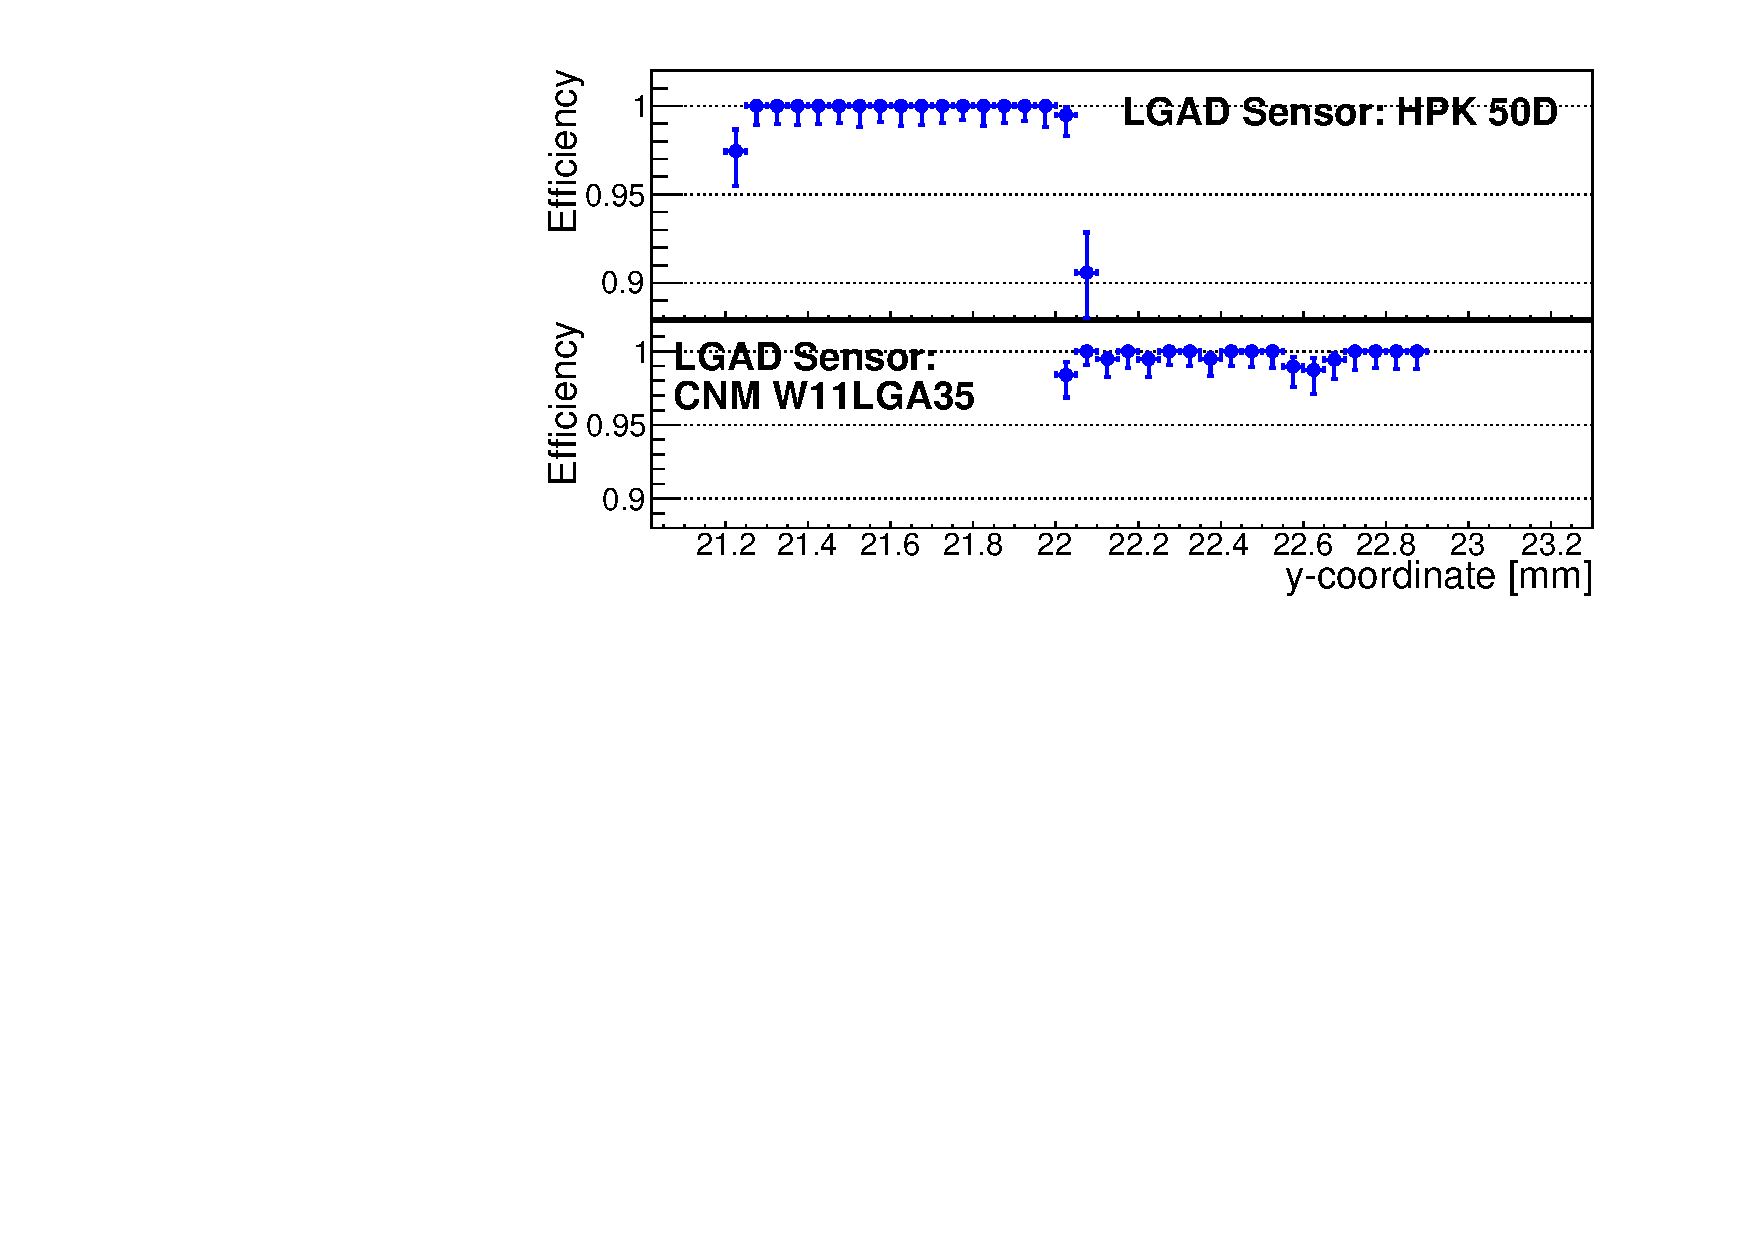
\includegraphics[width=0.90\textwidth]{figs/USCSBoard_HPK50DIrradiated-CNMW11LGA35_Run936-961/IrradiatedSensorStudy_Efficiency_vs_Y.pdf} 
\caption{Efficiency vs X and Y on CNM and HPK irradiated} 
\label{fig:Sensors} 
\end{figure} 

\begin{figure}[htbp] 
\centering
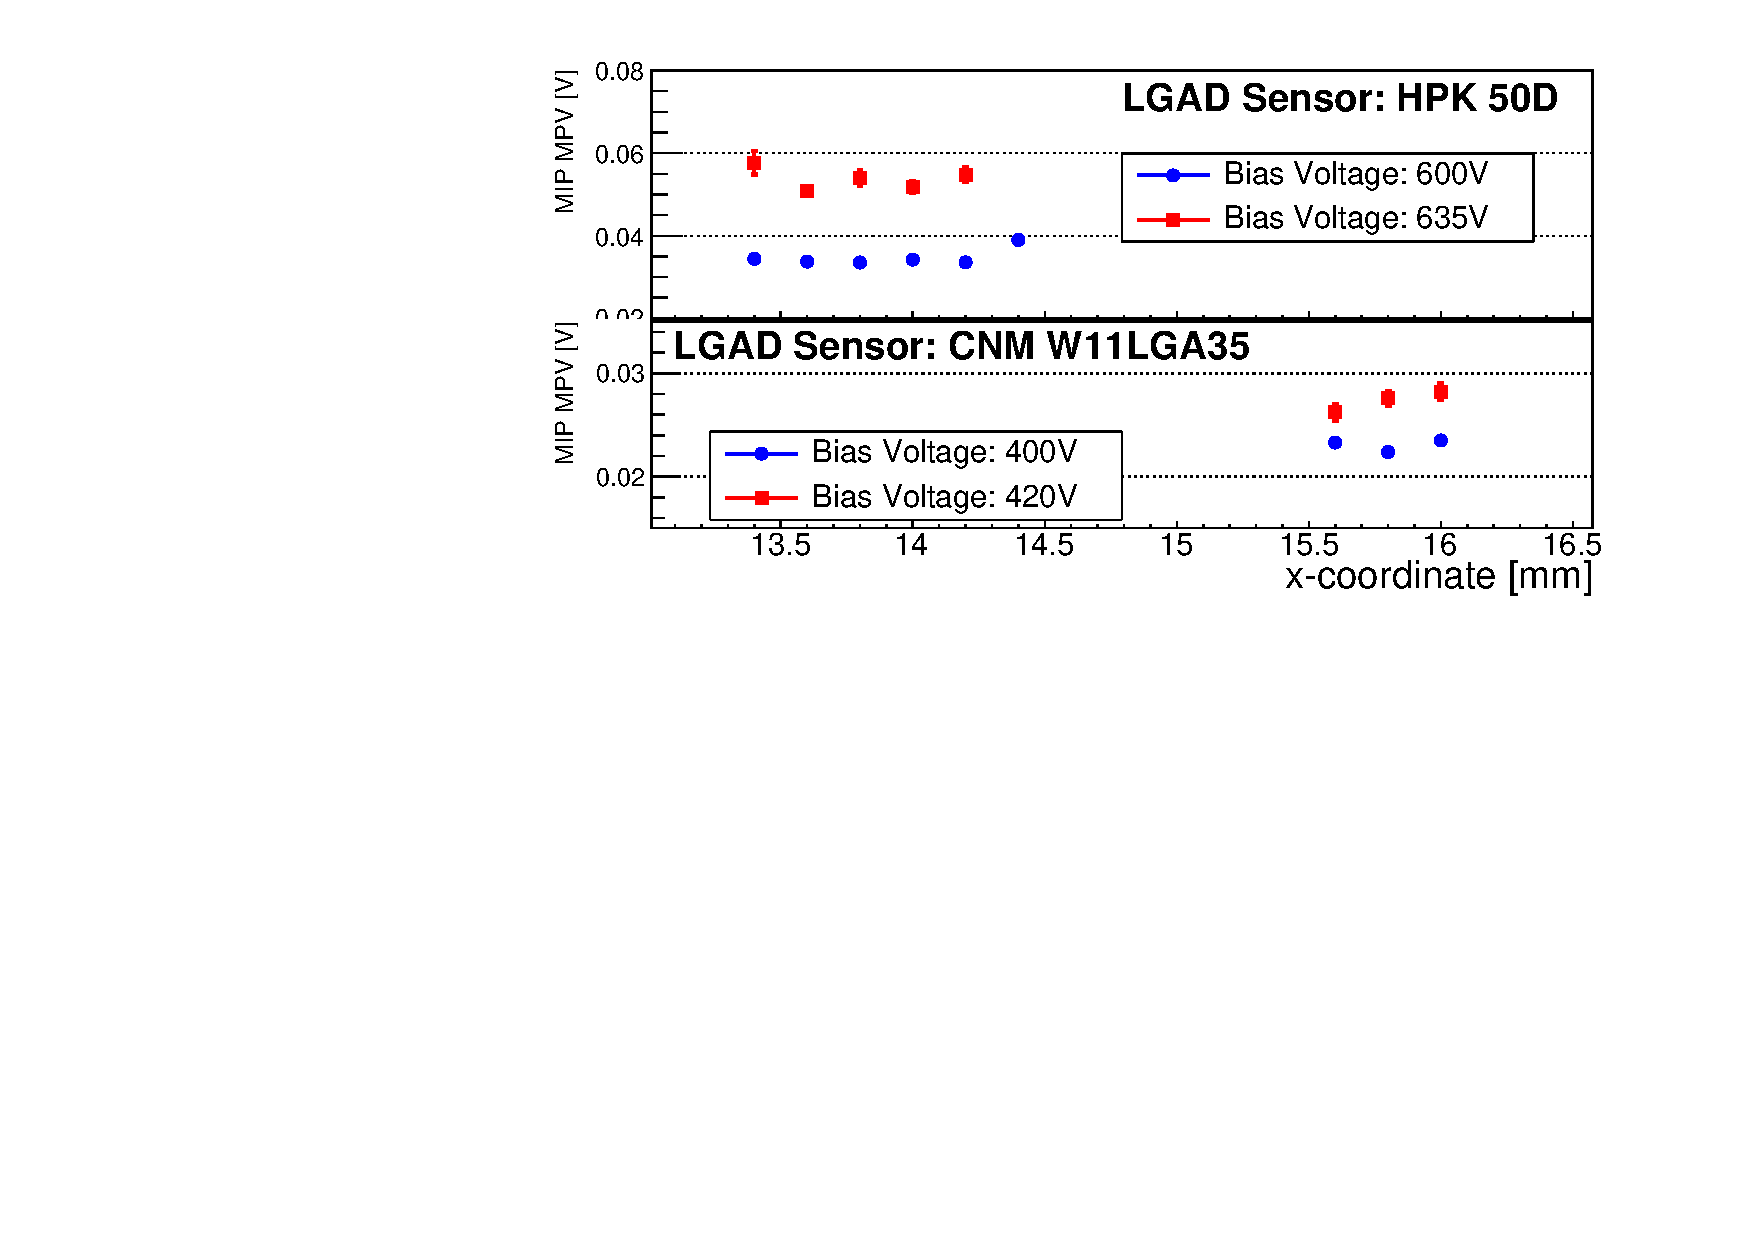
\includegraphics[width=0.90\textwidth]{figs/USCSBoard_HPK50DIrradiated-CNMW11LGA35_Run936-961/IrradiatedSensorStudy_MPV_vs_X.pdf} 
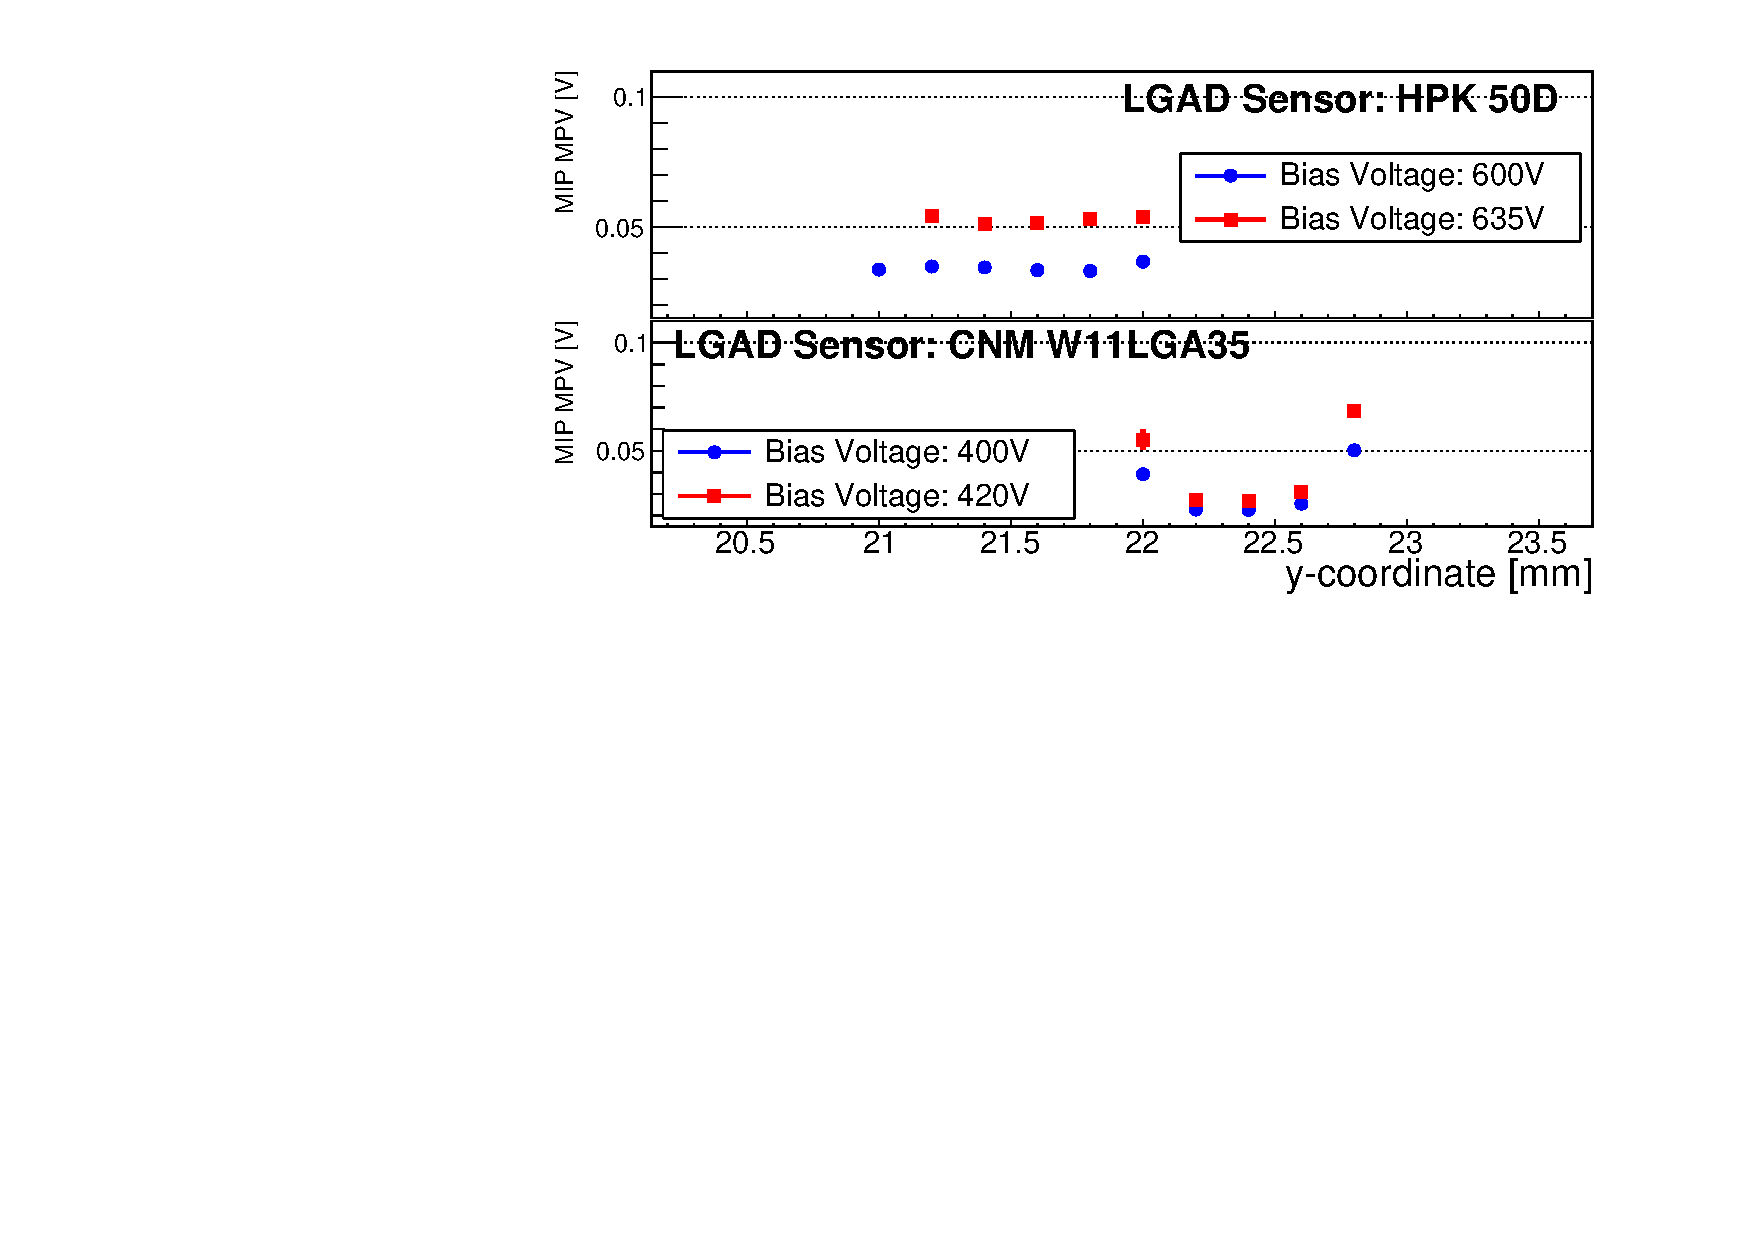
\includegraphics[width=0.90\textwidth]{figs/USCSBoard_HPK50DIrradiated-CNMW11LGA35_Run936-961/IrradiatedSensorStudy_MPV_vs_Y.pdf} 
\caption{MPV vs X and Y on CNM and HPK irradiated} 
\label{fig:Sensors} 
\end{figure}


\begin{figure}[htbp] 
\centering
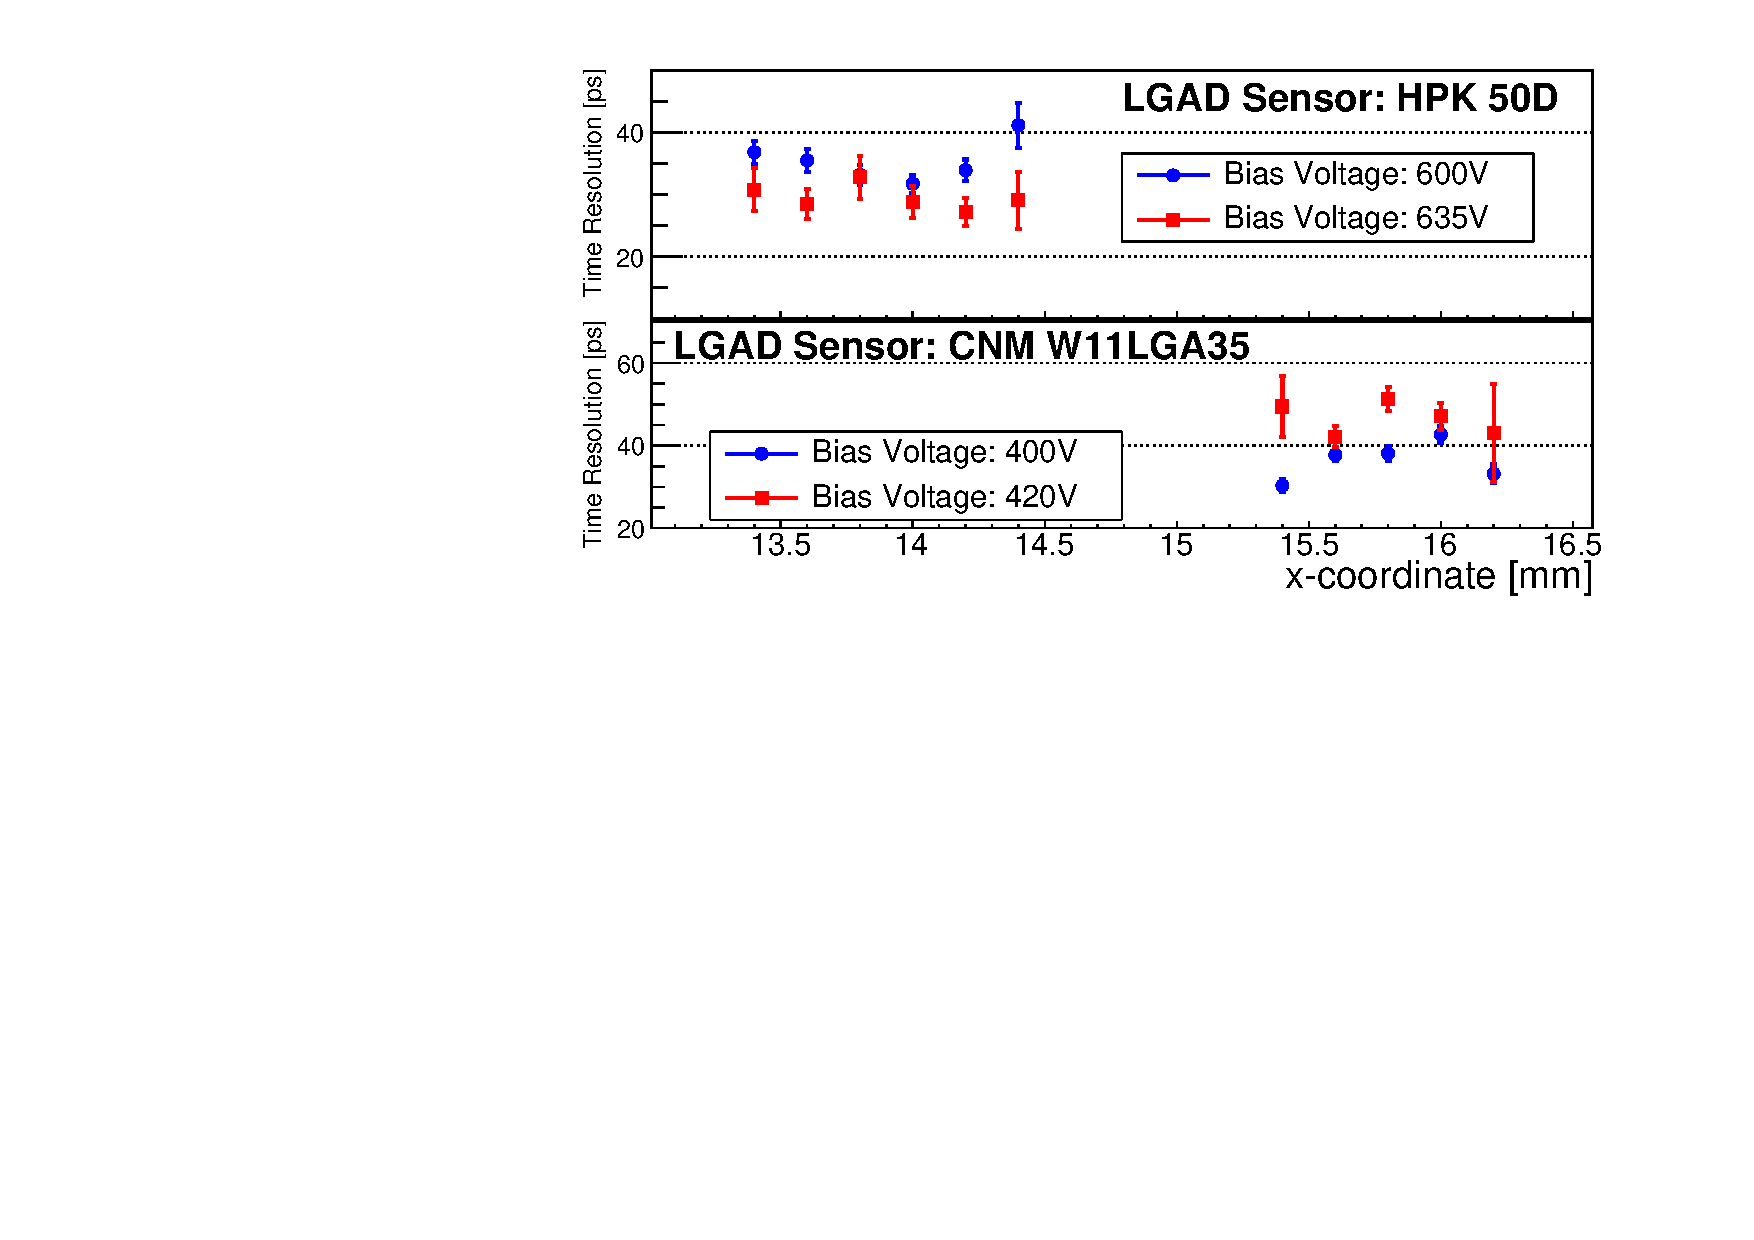
\includegraphics[width=0.90\textwidth]{figs/USCSBoard_HPK50DIrradiated-CNMW11LGA35_Run936-961/IrradiatedSensorStudy_TimeResolution_vs_X.pdf} 
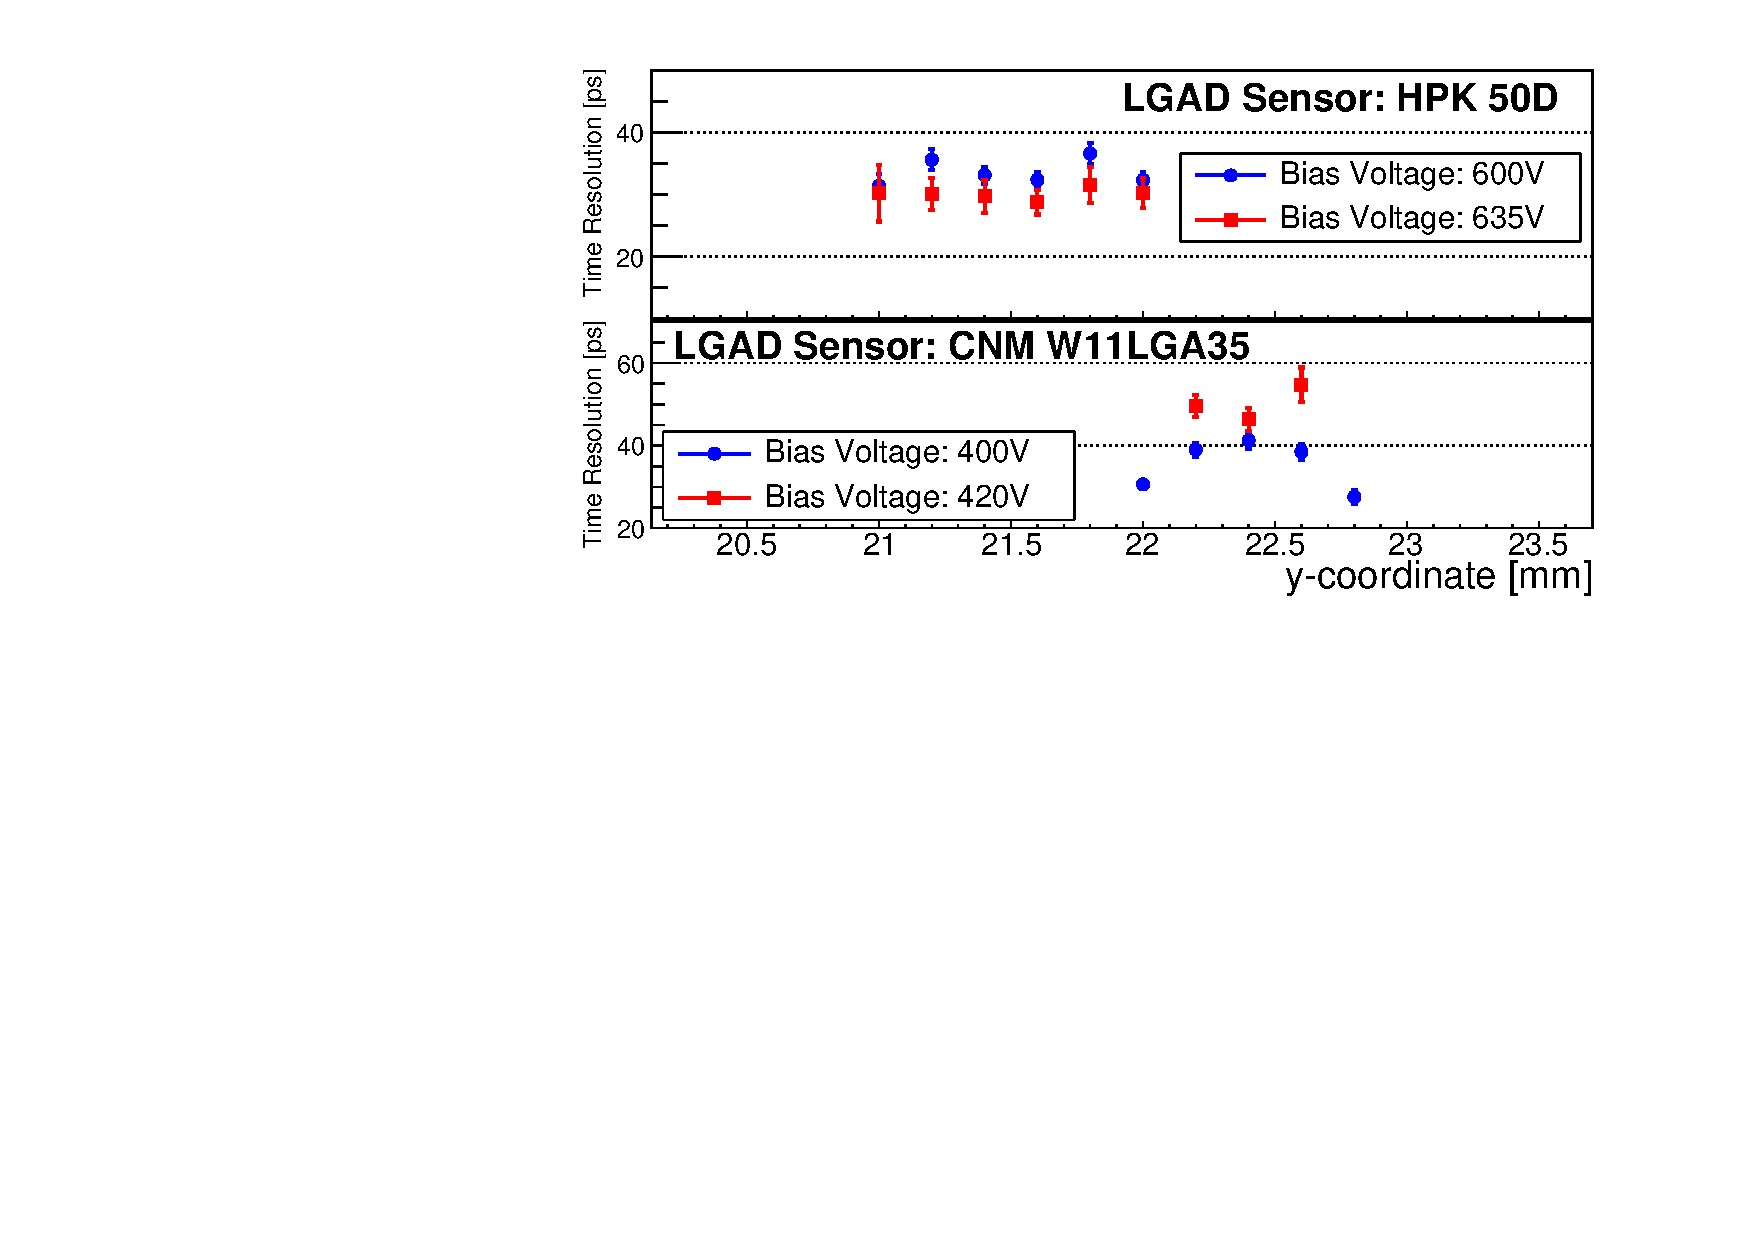
\includegraphics[width=0.90\textwidth]{figs/USCSBoard_HPK50DIrradiated-CNMW11LGA35_Run936-961/IrradiatedSensorStudy_TimeResolution_vs_Y.pdf} 
\caption{Time Resolution vs X and Y on CNM and HPK irradiated} 
\label{fig:Sensors} 
\end{figure} 

\begin{figure}[htbp] 
\centering
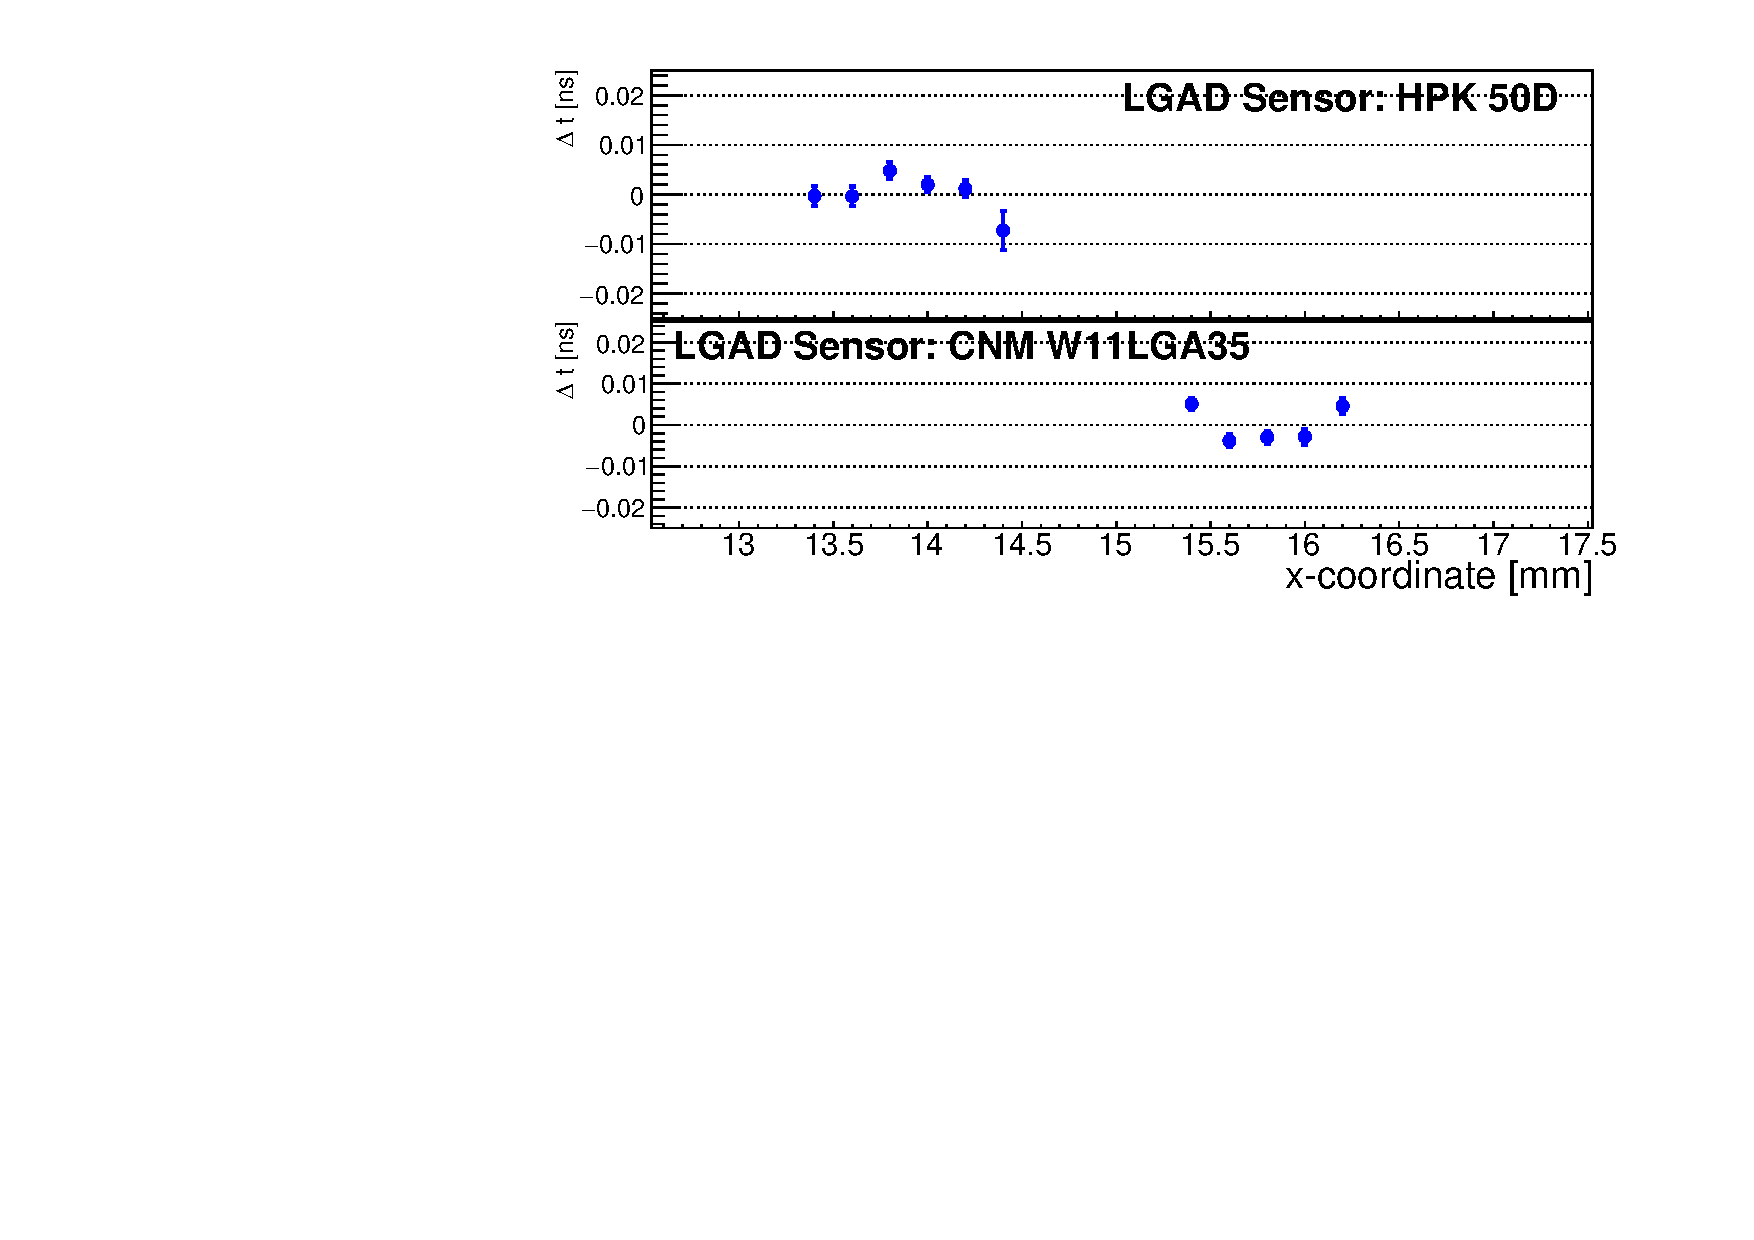
\includegraphics[width=0.9\textwidth]{figs/USCSBoard_HPK50DIrradiated-CNMW11LGA35_Run936-961/IrradiatedSensorStudy_MeanTime_vs_X.pdf} 
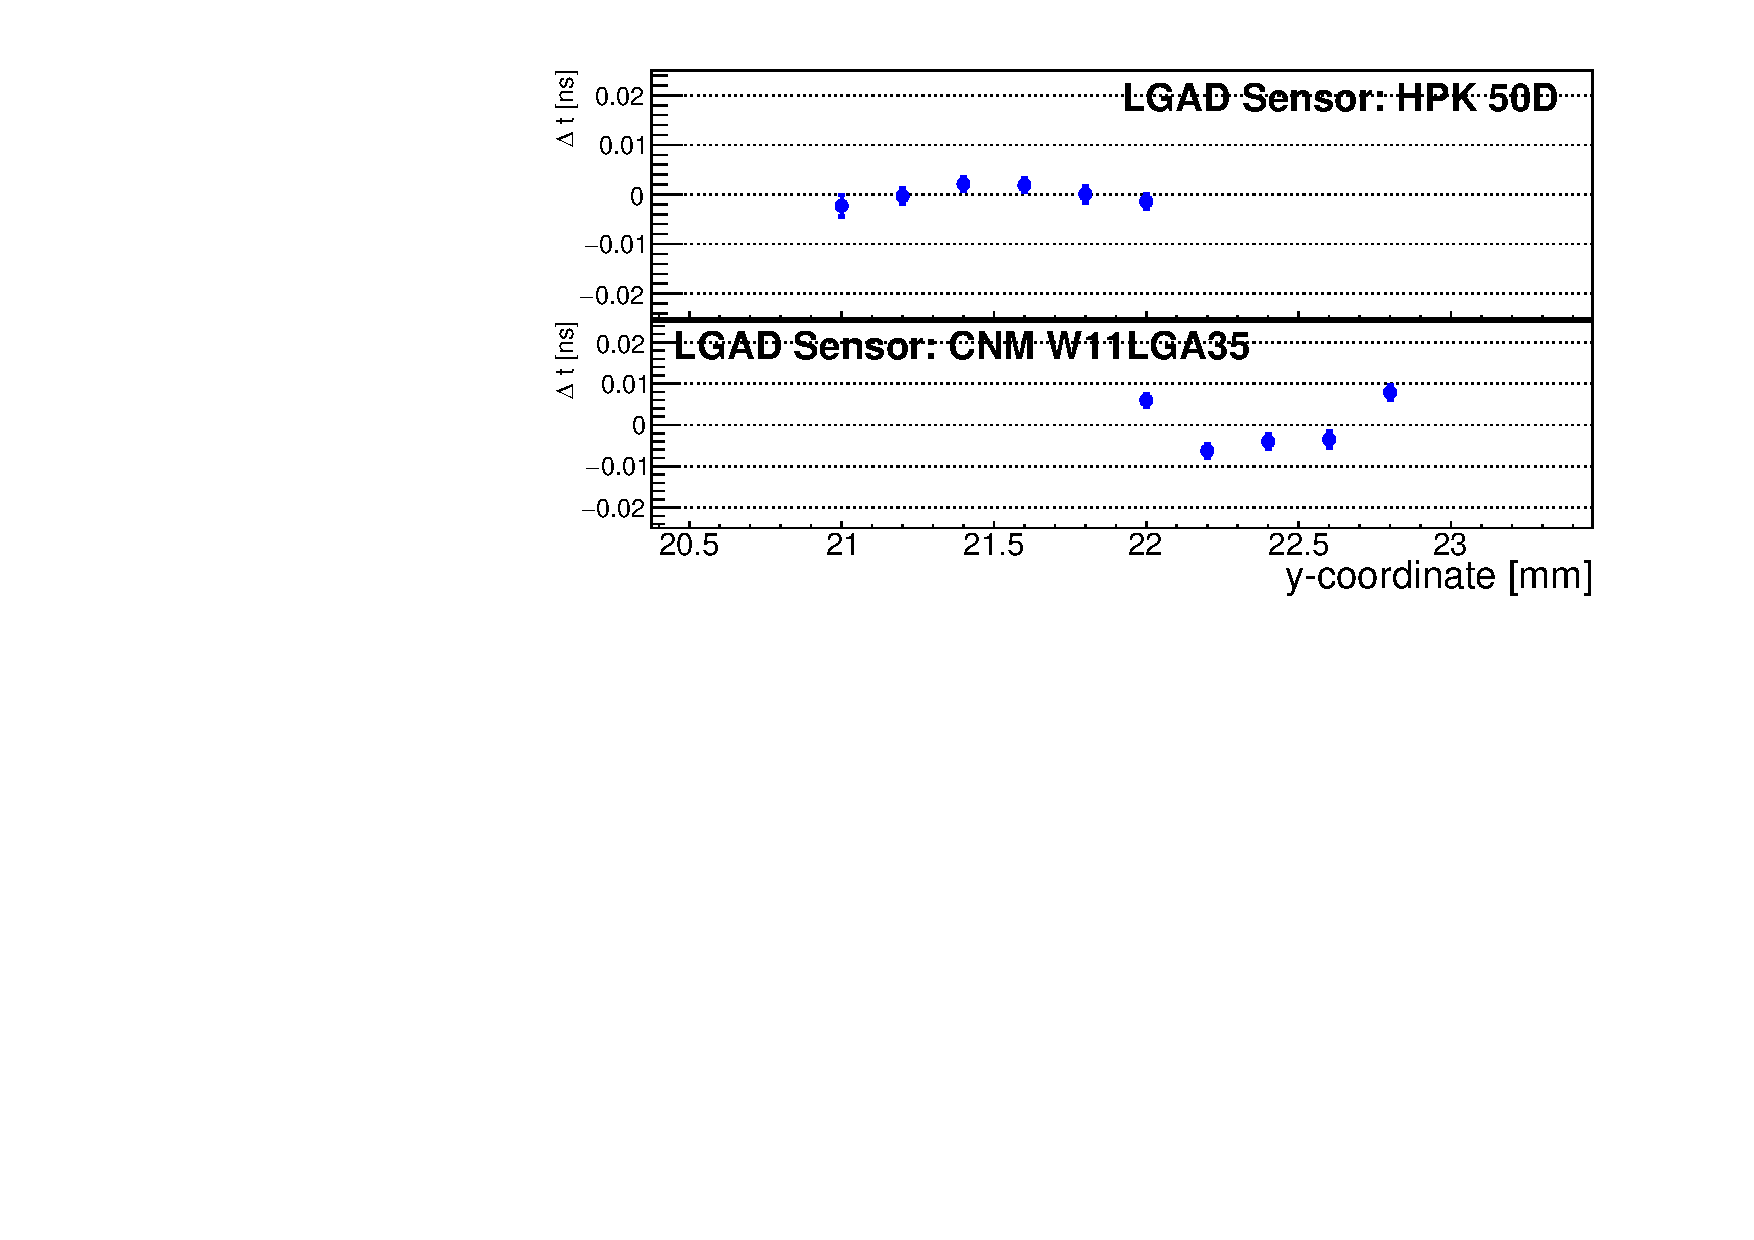
\includegraphics[width=0.9\textwidth]{figs/USCSBoard_HPK50DIrradiated-CNMW11LGA35_Run936-961/IrradiatedSensorStudy_MeanTime_vs_Y.pdf} 
\caption{DeltaT vs X and Y on CNM and HPK irradiated} 
\label{fig:Sensors} 
\end{figure} 
 



\clearpage
\section{Conclusion}
\label{sec:conclusion} 

All is good!

\section*{Acknowledgement}

We would like to thank Alan Prosser and Ryan Rivera for their critical help in
setting up the DAQ and trigger chain. 

%% The Appendices part is started with the command \appendix;
%% appendix sections are then done as normal sections
%% \appendix

%% \section{}
%% \label{}

%% If you have bibdatabase file and want bibtex to generate the
%% bibitems, please use
%%
%%  \bibliographystyle{elsarticle-num} 
%%  \bibliography{<your bibdatabase>}

%% else use the following coding to input the bibitems directly in the
%% TeX file.

\bibliography{LGAD_May2017_FNALTB}{}
\bibliographystyle{ieeetr} 

%\begin{thebibliography}{00}

%% \bibitem{label}
%% Text of bibliographic item

%\bibitem{}

%\end{thebibliography}
\end{document}
\endinput
%%
%% End of file `elsarticle-template-num.tex'.


























